% Tesi triennale - Politecnico di Milano
% Polarimetro a Immagine 2D Low-Cost per Polarimetria Spazialmente Risolta
% Filippo Narici - Ingegneria Fisica - A.A. 2025-26
%
% Template base: PoliMi3i (S. Bonetti, A. Gruttadauria, G. Mescolini, A. Zingaro)
% Copyright 2021 Politecnico di Milano, Italy. NC-BY

\documentclass{Configuration_Files/PoliMi3i_thesis}

%------------------------------------------------------------------------------
%	REQUIRED PACKAGES AND CONFIGURATIONS
%------------------------------------------------------------------------------

% CONFIGURATIONS
\usepackage{parskip} % For paragraph layout
\usepackage{setspace} % For using single or double spacing
\usepackage{emptypage} % To insert empty pages
\usepackage{multicol} % To write in multiple columns (executive summary)
\setlength\columnsep{15pt} % Column separation in executive summary
\setlength\parindent{0pt} % Indentation
\raggedbottom

% PACKAGES FOR TITLES
\usepackage{titlesec}
\titlespacing{\section}{0pt}{3.3ex}{2ex}
\titlespacing{\subsection}{0pt}{3.3ex}{1.65ex}
\titlespacing{\subsubsection}{0pt}{3.3ex}{1ex}
\usepackage{color}

% PACKAGES FOR LANGUAGE AND FONT
\usepackage[italian]{babel} % Tesi in italiano
\usepackage[utf8]{inputenc} % UTF8 encoding
\usepackage[T1]{fontenc} % Font encoding
\usepackage[11pt]{moresize} % Big fonts

% PACKAGES FOR IMAGES
\usepackage{graphicx}
\usepackage{transparent} % Enables transparent images
\usepackage{eso-pic} % For the background picture on the title page
\usepackage{subfig} % Numbered and caption subfigures using \subfloat
\usepackage{tikz} % A package for high-quality hand-made figures
\usetikzlibrary{arrows.meta, positioning}
\graphicspath{{./Images/}} % Directory of the images
\usepackage{caption} % Coloured captions
\usepackage{xcolor} % Coloured captions
\usepackage{amsthm,thmtools,xcolor} % Coloured "Theorem"
\usepackage{float}

% === Marcatori di revisione (TEMPORANEI, rimuovibili per colore) ===
% Ogni capitolo/blocco da revisionare e' colorato. Rivisto un colore -> rimuovere
% le righe \REVstart{<col>}/\REVend{<col>} corrispondenti in questo file.
\definecolor{revIntro}{rgb}{0.55,0.10,0.75}     % viola  - cap1 Introduzione
\definecolor{revTeoria}{rgb}{0.10,0.25,0.85}    % blu    - cap2 Teoria
\definecolor{revSetup}{rgb}{0.00,0.55,0.20}     % verde  - cap3 Apparato + cap4 Campioni
\definecolor{revAnalisi}{rgb}{0.90,0.45,0.00}   % arancio- cap5 Analisi
\definecolor{revRisultati}{rgb}{0.80,0.05,0.05} % rosso  - cap6 Risultati
\definecolor{revConcl}{rgb}{0.00,0.50,0.50}     % teal   - cap7 Conclusioni
\newcommand{\REVstart}[1]{\color{#1}}
\newcommand{\REVend}[1]{\color{black}}

% STANDARD MATH PACKAGES
\usepackage{amsmath}
\usepackage{amsthm}
\usepackage{amssymb}
\usepackage{amsfonts}
\usepackage{bm}
\usepackage[overload]{empheq} % For braced-style systems of equations
\usepackage{fix-cm} % To override original LaTeX restrictions on sizes

% PACKAGES FOR TABLES
\usepackage{tabularx}
\usepackage{longtable} % Tables that can span several pages
\usepackage{colortbl}

% PACKAGES FOR ALGORITHMS (PSEUDO-CODE)
\usepackage{algorithm}
\usepackage{algorithmic}

% PACKAGES FOR REFERENCES & BIBLIOGRAPHY
\usepackage[colorlinks=true,linkcolor=black,anchorcolor=black,citecolor=black,filecolor=black,menucolor=black,runcolor=black,urlcolor=black]{hyperref}
\usepackage[italian]{cleveref}
\usepackage[square, numbers, sort&compress]{natbib}
\bibliographystyle{abbrvnat}

% OTHER PACKAGES
\usepackage{pdfpages} % To include a pdf file
\usepackage{afterpage}
\usepackage{fancyhdr} % For the headers
\fancyhf{}

% Input of configuration file
\input{Configuration_Files/config}

%------------------------------------------------------------------------------
%	NEW COMMANDS DEFINED
%------------------------------------------------------------------------------

\newcommand{\bea}{\begin{eqnarray}}
\newcommand{\eea}{\end{eqnarray}}
\newcommand{\e}[1]{\times 10^{#1}}

%------------------------------------------------------------------------------
%	ADD YOUR PACKAGES
%------------------------------------------------------------------------------

\usepackage{siunitx} % Unita' SI

%------------------------------------------------------------------------------
%	ADD YOUR DEFINITIONS AND COMMANDS
%------------------------------------------------------------------------------

% Vettore di Stokes
\newcommand{\Svec}{\mathbf{S}}
% Matrice di Mueller
\newcommand{\Mmat}{\mathbf{M}}

%------------------------------------------------------------------------------
%	BEGIN OF YOUR DOCUMENT
%------------------------------------------------------------------------------

\begin{document}

\fancypagestyle{plain}{%
\fancyhf{} % Clear all header and footer fields
\fancyhead[RO,RE]{\thepage} %RO=right odd, RE=right even
\renewcommand{\headrulewidth}{0pt}
\renewcommand{\footrulewidth}{0pt}}

%------------------------------------------------------------------------------
%	TITLE PAGE
%------------------------------------------------------------------------------

\pagestyle{empty} % No page numbers
\frontmatter % Use roman page numbering style (i, ii, iii, iv...)

\puttitle{
	title=Polarimetro a Immagine 2D Low-Cost per Polarimetria Full-Stokes Spazialmente Risolta,
	name=Filippo Narici,
	course=Ingegneria Fisica,
	ID=211644,
	advisor=Prof. Maurizio Zani,
	coadvisor={Sebastiano Luridiana, Giacomo Di Iorio},
	academicyear={2025-26},
}

%------------------------------------------------------------------------------
%	PREAMBLE PAGES: ABSTRACT
%------------------------------------------------------------------------------
\startpreamble
\setcounter{page}{1}

% ABSTRACT
\chapter*{Abstract}
La polarimetria --- la misura quantitativa dello stato di polarizzazione della luce --- è uno strumento trasversale a ottica, scienza dei materiali e ingegneria strutturale. Gli apparati convenzionali, tuttavia, forniscono misure puntuali e hanno costi dell'ordine delle decine di migliaia di euro, limitandone l'impiego ai laboratori specializzati.

Questa tesi presenta la progettazione e la validazione di un polarimetro a immagine bidimensionale a basso costo, in cui il sensore CMOS di uno smartphone commerciale sostituisce il rivelatore tradizionale. Il sistema acquisisce 36 immagini a passi angolari regolari dell'analizzatore e due misure aggiuntive con una lamina quarto d'onda; il vettore di Stokes completo viene poi ricostruito pixel per pixel mediante regressione ai minimi quadrati. Si ottengono cos\`i mappe spazialmente risolte della polarizzazione lineare e circolare, della ritardanza e dell'orientazione dell'asse veloce sull'intero campo visivo.

% DA RIVEDERE MANUALMENTE (abstract riallineato a cap6 il 2026-07-03, post peer review interna)
L'apparato è stato validato su campioni rappresentativi di birifrangenza (lamine d'onda commerciali, strati di nastro adesivo), attività ottica (soluzione di saccarosio) e fotoelasticità (righello in plastica, trave a sbalzo sotto carico). La correzione cromatica di $S_3$ è calibrata direttamente dai dati, senza assunzioni sul materiale della lamina impiegata come analizzatore. La lamina quarto d'onda segue la legge di dispersione di un ritardatore a singolo ordine entro pochi gradi; la lamina mezz'onda viene riconosciuta come ritardatore a dispersione di ritardanza inversa, della famiglia a largo spettro, informazione non deducibile dall'etichetta e indice della capacità diagnostica spettrale del metodo; il nastro adesivo stratificato conferma la linearità della risposta fino a oltre $1500^\circ$ di ritardanza accumulata; la rotazione ottica della soluzione di saccarosio mostra una dispersione descritta in prima approssimazione dal modello di Drude. I risultati dimostrano che un apparato il cui costo, escluso lo smartphone, è inferiore a 100\,\texteuro, è in grado di produrre mappe polarimetriche bidimensionali quantitative, rendendolo un'alternativa concreta agli strumenti di laboratorio convenzionali per la didattica e la ricerca esplorativa.
\\
\\
\textbf{Parole chiave:} polarimetria a immagine, parametri di Stokes, sensore CMOS smartphone, birifrangenza, fotoelasticit\`a, strumentazione low-cost

%------------------------------------------------------------------------------
%	LIST OF CONTENTS/FIGURES/TABLES
%------------------------------------------------------------------------------

\thispagestyle{empty}
\tableofcontents
\thispagestyle{empty}
\cleardoublepage

%------------------------------------------------------------------------------
%	THESIS MAIN TEXT
%------------------------------------------------------------------------------

\addtocontents{toc}{\vspace{2em}}
\mainmatter % Begin numeric (1,2,3...) page numbering

% --------------------------------------------------------------------------
% CAPITOLI
% --------------------------------------------------------------------------

\chapter{Introduzione}
\label{ch:introduzione}
\REVstart{revIntro}
% Capitolo 1: Introduzione

La polarizzazione della luce descrive l'orientazione e il comportamento temporale del campo elettrico nel piano trasversale alla direzione di propagazione.A differenza dell’intensità e della frequenza, la polarizzazione non è direttamente percepibile, ma codifica informazioni essenziali sulle proprietà del mezzo attraversato: struttura cristallina, stato di sollecitazione meccanica, chiralità molecolare. La polarimetria, ossia la misura quantitativa dello stato di polarizzazione, è per questa ragione uno strumento trasversale a ottica, scienza dei materiali, chimica analitica e ingegneria strutturale, con applicazioni in fotoelasticità, diagnostica biomedica, controllo qualità industriale e osservazione astronomica.


\section{Dalla misura puntuale all'immagine}
\label{sec:polarimetria_classica}
L'approccio tradizionale alla polarimetria impiega un rivelatore puntuale (tipicamente un fotodiodo) posto dietro un sistema di analizzatore e lamine ritardatrici. Ruotando l'analizzatore si ricostruiscono i quattro parametri di Stokes del fascio incidente: configurazione descritta, ad esempio, nel manuale di laboratorio del corso di Fisica Sperimentale del Politecnico di Milano~\cite{manuale_polarizzazione}, preso come punto di partenza per questa tesi. Il limite principale di questo schema è la sua natura \emph{zero-dimensionale}: il rivelatore fornisce una singola misura scalare, integrata sull'intera sezione del fascio. Se il campione presenta variazioni spaziali delle proprietà ottiche, come accade nella maggior parte delle situazioni di interesse pratico, l'informazione spaziale viene irrimediabilmente perduta. Un secondo limite, per quanto meno stringente, è economico: un polarimetro di Stokes puntuale di grado commerciale, in cui un analizzatore o una lamina ritardatrice motorizzata ruota davanti a un fotodiodo, ha un costo dell'ordine di alcune migliaia di euro.

L'idea di sostituire il rivelatore puntuale con un sensore a matrice trasforma il polarimetro da strumento scalare a strumento di imaging: ogni pixel diventa un polarimetro indipendente, e la misura restituisce una mappa bidimensionale dello stato di polarizzazione. Le soluzioni commerciali per questo scopo si distribuiscono in due famiglie con prestazioni e costi assai diversi. Le telecamere a divisione del piano focale, costruite attorno a un array di micro-polarizzatori integrato direttamente sul sensore CMOS, forniscono mappe di polarizzazione in un singolo scatto a un costo di alcune migliaia di euro, ma misurano la sola polarizzazione lineare ($S_0$, $S_1$, $S_2$): l'assenza di elementi ritardatori sul piano focale impedisce loro l'accesso alla componente circolare $S_3$. La misura del vettore di Stokes completo su un campo bidimensionale richiede invece sistemi attivi, con modulatori a cristalli liquidi o compensatori rotanti motorizzati. % TODO: vero? questi strumenti esistono davvero? poi frase sembra implicare due famiglie ma la seconda famiglia sembra introdotta con una frase a parte

% TODO: rifare paragrafo sotto, prima dicono che sono a basso costo poi che costano migliaia di euro, inoltre andrebbe verificato fulltext delle fonti, le allego in biblio
Strumenti polarimetrici a basso costo basati su smartphone sono già documentati in letteratura per la spettropolarimetria atmosferica~\cite{Burggraaff2020ispex}, per la diagnostica biomedica~\cite{Gonzalez2020colposcope,Louie2021skin} e nella didattica della fisica~\cite{Gallitto2024malus,Bernard2020polarimeter}, mentre la ricostruzione dell'intero vettore di Stokes a immagine in un singolo scatto è oggetto di ricerca recente~\cite{Baek2022lensless,Gu2022fullstokes}. Un prodotto commerciale capace di quest'ultima misura ha un costo dell'ordine delle decine di migliaia di euro e resta accessibile soprattutto ai laboratori ben attrezzati.

% TODO: trovo riduttivo parlare di studenti, questo è un lavoro utle in generale
La diffusione capillare degli smartphone, con sensori CMOS ad alta risoluzione e acquisizione RAW, suggerisce una possibilità concreta: impiegare come rivelatore un dispositivo già posseduto dalla quasi totalità degli studenti per ottenere mappe del vettore di Stokes completo a un costo dell'ordine delle centinaia di euro, due ordini di grandezza inferiore a quello dei sistemi commerciali capaci della stessa misura.


\section{Obiettivo del lavoro}
\label{sec:obiettivo}

Questa tesi si propone di progettare, realizzare e validare un polarimetro a immagine bidimensionale a basso costo, utilizzando come rivelatore il sensore CMOS di uno smartphone commerciale. Il sistema deve ricostruire il vettore di Stokes completo pixel per pixel e generare mappe spazialmente risolte del grado di polarizzazione, dell'angolo di polarizzazione lineare, della ritardanza e dell'orientazione dell'asse veloce. Per validarne le capacità, vengono analizzati campioni rappresentativi di birifrangenza, attività ottica e fotoelasticità.

Il \cref{ch:teoria} richiama i fondamenti teorici necessari alla comprensione del metodo di misura. Il \cref{ch:apparato} descrive l'apparato sperimentale e il protocollo di acquisizione. Il \cref{ch:campioni} presenta i campioni selezionati. Il \cref{ch:analisi} documenta l'analisi dei dati. Il \cref{ch:risultati} discute i risultati e i limiti del metodo. Il \cref{ch:conclusioni} riassume le conclusioni e indica possibili sviluppi futuri.

\REVend{revIntro}

\chapter{Fondamenti teorici della polarimetria}
\label{ch:teoria}
\REVstart{revTeoria}
% Capitolo 2: Fondamenti teorici della polarimetria

\section{Polarizzazione della luce}
\label{sec:polarizzazione}

La luce è un'onda elettromagnetica trasversale. Per un'onda monocromatica che si propaga lungo l'asse $z$, il campo elettrico può essere decomposto in due componenti ortogonali $E_x$ e $E_y$, ciascuna con ampiezza e fase proprie~\cite{hecht2017optics}. La differenza di fase $\delta = \delta_y - \delta_x$ tra le due componenti determina lo stato di polarizzazione: quando $\delta = 0$ o $\pi$ la polarizzazione è lineare, quando $\delta = \pm\pi/2$ con ampiezze uguali è circolare, e nel caso generale è ellittica. Le sorgenti comuni emettono luce non polarizzata, in cui $\delta$ varia casualmente nel tempo; la sovrapposizione di una componente polarizzata e una non polarizzata produce luce parzialmente polarizzata, situazione tipica in ambito sperimentale.


\section{Formalismo di Stokes}
\label{sec:stokes}

Per descrivere la polarizzazione della luce esistono diversi formalismi. Il \emph{formalismo di Jones}, basato su un vettore complesso a due componenti, è efficace ma limitato alla luce completamente polarizzata. Per trattare anche la luce parzialmente polarizzata, situazione comune nella pratica sperimentale, è necessario un formalismo più generale: il \textbf{formalismo di Stokes}, introdotto da George Gabriel Stokes nel 1852~\cite{goldstein2011polarized}.

\subsection{Definizione dei parametri di Stokes}
\label{subsec:stokes_def}

I quattro parametri di Stokes si definiscono a partire dalle componenti del campo elettrico attraverso medie temporali~\cite{collett2005polarized}:
\begin{equation}
\label{eq:stokes_campi}
\Svec = \begin{pmatrix} S_0 \\ S_1 \\ S_2 \\ S_3 \end{pmatrix} = \begin{pmatrix} \langle E_{0x}^2 \rangle + \langle E_{0y}^2 \rangle \\ \langle E_{0x}^2 \rangle - \langle E_{0y}^2 \rangle \\ 2\langle E_{0x} E_{0y} \cos\delta \rangle \\ 2\langle E_{0x} E_{0y} \sin\delta \rangle \end{pmatrix},
\end{equation}
dove le parentesi angolari indicano la media temporale. $S_0$ rappresenta l'intensità totale del fascio; $S_1$ quantifica la prevalenza della polarizzazione orizzontale ($S_1 > 0$) o verticale ($S_1 < 0$); $S_2$ la prevalenza della polarizzazione a $+45^\circ$ ($S_2 > 0$) o $-45^\circ$ ($S_2 < 0$); $S_3$ la prevalenza della polarizzazione circolare destra ($S_3 > 0$) o sinistra ($S_3 < 0$). I parametri di Stokes sono quantità misurabili, proporzionali alle intensità registrate da combinazioni appropriate di polarizzatori e lamine:
\begin{equation}
\label{eq:stokes_intensita}
\Svec = \begin{pmatrix} I_H + I_V \\ I_H - I_V \\ I_{+45} - I_{-45} \\ I_{RCP} - I_{LCP} \end{pmatrix},
\end{equation}
dove $I_H$, $I_V$, $I_{+45}$, $I_{-45}$ sono le intensità trasmesse da polarizzatori lineari orientati rispettivamente a $0^\circ$, $90^\circ$, $+45^\circ$ e $-45^\circ$, mentre $I_{RCP}$ e $I_{LCP}$ corrispondono alle componenti circolare destra e sinistra.

Per qualsiasi stato di polarizzazione vale la disuguaglianza fondamentale:
\begin{equation}
\label{eq:stokes_disuguaglianza}
S_0^2 \geq S_1^2 + S_2^2 + S_3^2,
\end{equation}
con l'uguaglianza valida esclusivamente per luce totalmente polarizzata. Il \textbf{grado di polarizzazione} (DOP, dall'inglese \textit{Degree of Polarization}) quantifica la frazione di luce polarizzata~\cite{bornwolf1999}:
\begin{equation}
\label{eq:DOP}
\text{DOP} = \frac{\sqrt{S_1^2 + S_2^2 + S_3^2}}{S_0},
\end{equation}
e vale 1 per luce totalmente polarizzata e 0 per luce completamente non polarizzata.

Dal punto di vista sperimentale, $S_0$, $S_1$ e $S_2$ si ottengono da misure di intensità attraverso un analizzatore lineare a diversi angoli, come mostrato dalla legge di Malus generalizzata (\cref{sec:malus}). Il parametro $S_3$ richiede l'inserimento di una lamina $\lambda/4$ prima dell'analizzatore.

\subsection{La sfera di Poincaré}
\label{subsec:poincare}

I parametri di Stokes normalizzati $s_1 = S_1/S_0$, $s_2 = S_2/S_0$, $s_3 = S_3/S_0$ definiscono un punto nello spazio tridimensionale. Gli stati totalmente polarizzati giacciono sulla superficie di una sfera unitaria --- la \textbf{sfera di Poincaré}~\cite{goldstein2011polarized} --- il cui equatore rappresenta la polarizzazione lineare e i cui poli rappresentano la polarizzazione circolare destra e sinistra. La distanza dal centro è pari al grado di polarizzazione. Questa rappresentazione geometrica sarà utile nell'interpretazione delle mappe di Stokes del \cref{ch:risultati}.


\section{Legge di Malus generalizzata}
\label{sec:malus}

La legge di Malus classica descrive l'intensità trasmessa da un polarizzatore ideale quando luce linearmente polarizzata lo attraversa. Se l'angolo tra la direzione di polarizzazione della luce incidente e l'asse di trasmissione dell'analizzatore è $\theta$, l'intensità trasmessa vale~\cite{hecht2017optics}:
\begin{equation}
\label{eq:malus_classica}
I(\theta) = I_0 \cos^2\theta.
\end{equation}

Nel caso di luce parzialmente polarizzata, la legge si generalizza utilizzando il formalismo di Stokes. L'intensità trasmessa da un analizzatore lineare ideale orientato a un angolo $\theta$ è~\cite{goldstein2011polarized}:
\begin{equation}
\label{eq:malus_generalizzata}
I(\theta) = \frac{1}{2}\bigl(S_0 + S_1\cos 2\theta + S_2\sin 2\theta\bigr).
\end{equation}
L'\cref{eq:malus_generalizzata} può essere derivata applicando la matrice di Mueller di un polarizzatore lineare ruotato di $\theta$ al vettore di Stokes incidente e leggendo la componente $S_0'$ del vettore uscente (il formalismo delle matrici di Mueller è introdotto nella \cref{sec:mueller}). Si osservi che l'intensità trasmessa dipende solo dai primi tre parametri di Stokes e non da $S_3$: un polarizzatore lineare è insensibile alla polarizzazione circolare.

Acquisendo $N$ immagini a diversi angoli $\theta_i$ dell'analizzatore, l'\cref{eq:malus_generalizzata} fornisce un sistema sovradeterminato di equazioni lineari nei tre parametri incogniti $S_0$, $S_1$ e $S_2$, risolvibile tramite il metodo della pseudo-inversa.


\section{Matrici di Mueller}
\label{sec:mueller}

Il formalismo delle matrici di Mueller descrive la trasformazione dello stato di polarizzazione della luce al passaggio attraverso un elemento ottico. Il vettore di Stokes uscente $\Svec_\text{out}$ è legato a quello incidente $\Svec_\text{in}$ dalla relazione~\cite{goldstein2011polarized}:
\begin{equation}
\label{eq:mueller}
\Svec_\text{out} = \Mmat \, \Svec_\text{in},
\end{equation}
dove $\Mmat$ è una matrice reale $4 \times 4$ caratteristica dell'elemento ottico. Per un sistema composto da $N$ elementi ottici in sequenza, la matrice complessiva si ottiene per moltiplicazione:
\begin{equation}
\label{eq:mueller_composizione}
\Mmat_\text{tot} = \Mmat_N \cdots \Mmat_2 \, \Mmat_1,
\end{equation}
dove $\Mmat_1$ è la matrice del primo elemento incontrato dal fascio.

\subsection{Polarizzatore lineare ideale}
\label{subsec:mueller_pol}

La matrice di Mueller di un polarizzatore lineare ideale con asse di trasmissione orizzontale è:
\begin{equation}
\label{eq:mueller_pol}
\Mmat_\text{pol}(0^\circ) = \frac{1}{2}\begin{pmatrix} 1 & 1 & 0 & 0 \\ 1 & 1 & 0 & 0 \\ 0 & 0 & 0 & 0 \\ 0 & 0 & 0 & 0 \end{pmatrix}.
\end{equation}
Per un polarizzatore con asse ruotato di un angolo $\theta$, la matrice si ottiene applicando la trasformazione di rotazione $\Mmat_\text{pol}(\theta) = \Mmat_R(-\theta)\,\Mmat_\text{pol}(0^\circ)\,\Mmat_R(\theta)$, dove $\Mmat_R(\theta)$ è la matrice di rotazione nello spazio di Stokes (\cref{eq:mueller_rotatore}).

\subsection{Lamina a ritardo (retarder)}
\label{subsec:mueller_retarder}

Una lamina a ritardo introduce una differenza di fase $\delta$ tra le componenti del campo polarizzate lungo l'asse veloce e l'asse lento. La matrice di Mueller per una lamina con asse veloce orizzontale è~\cite{collett2005polarized}:
\begin{equation}
\label{eq:mueller_retarder}
\Mmat_\text{ret}(\delta) = \begin{pmatrix} 1 & 0 & 0 & 0 \\ 0 & 1 & 0 & 0 \\ 0 & 0 & \cos\delta & \sin\delta \\ 0 & 0 & -\sin\delta & \cos\delta \end{pmatrix}.
\end{equation}
I casi di interesse principale sono la lamina \textbf{quarto d'onda} ($\delta = \pi/2$) e la lamina \textbf{mezzo d'onda} ($\delta = \pi$). Per una lamina con asse veloce ruotato di un angolo $\alpha$, si applica la stessa trasformazione di rotazione descritta per il polarizzatore.

\subsection{Rotatore ottico}
\label{subsec:mueller_rotatore}

Un rotatore ottico ruota il piano di polarizzazione di un angolo $\phi$ senza modificare l'ellitticità. La sua matrice di Mueller è~\cite{goldstein2011polarized}:
\begin{equation}
\label{eq:mueller_rotatore}
\Mmat_R(\phi) = \begin{pmatrix} 1 & 0 & 0 & 0 \\ 0 & \cos 2\phi & \sin 2\phi & 0 \\ 0 & -\sin 2\phi & \cos 2\phi & 0 \\ 0 & 0 & 0 & 1 \end{pmatrix}.
\end{equation}
Il fattore $2\phi$ riflette la periodicità $\pi$ della polarizzazione lineare: una rotazione fisica di $\phi$ corrisponde a uno spostamento di $2\phi$ sulla sfera di Poincaré.


\section{Fenomeni che influenzano la polarizzazione}
\label{sec:fenomeni}

I campioni analizzati in questa tesi interagiscono con la polarizzazione attraverso tre meccanismi distinti, ciascuno descritto da una specifica matrice di Mueller.

\textbf{Birifrangenza.} Un materiale è birifrangente quando il suo indice di rifrazione dipende dalla direzione di polarizzazione. Nei cristalli uniassici si distinguono l'indice \textbf{ordinario} $n_o$ e l'indice \textbf{straordinario} $n_e$; la differenza $\Delta n = n_e - n_o$ è la birifrangenza del materiale~\cite{hecht2017optics}. Quando un'onda polarizzata attraversa un mezzo birifrangente di spessore $d$, le due componenti del campo accumulano una differenza di fase detta \textbf{ritardanza}:
\begin{equation}
\label{eq:ritardanza}
\delta = \frac{2\pi}{\lambda}\,\Delta n\, d,
\end{equation}
dove $\lambda$ è la lunghezza d'onda nel vuoto. Le \textbf{lamine d'onda} sfruttano questo effetto: una lamina $\lambda/4$ ($\delta = \pi/2$) converte polarizzazione lineare a $45^\circ$ in circolare, una lamina $\lambda/2$ ($\delta = \pi$) ruota il piano di polarizzazione di un angolo doppio rispetto all'orientazione della lamina. Poiché $\delta$ dipende inversamente da $\lambda$, una lamina calibrata a una data lunghezza d'onda introduce ritardi diversi alle altre lunghezze d'onda --- un aspetto che avrà conseguenze dirette sulla misura di $S_3$ con il sensore a tre canali colore (\cref{ch:analisi}). Una lamina \textbf{zero-order}, il cui ritardo è ottenuto con un singolo passaggio attraverso un cristallo sottile, presenta una dipendenza dalla lunghezza d'onda più debole rispetto a una lamina \textbf{multi-order}.

\textbf{Attività ottica.} Alcuni materiali chirali ruotano il piano di polarizzazione senza alterare l'ellitticità: nel formalismo di Mueller, l'effetto corrisponde a un rotatore (\cref{eq:mueller_rotatore}), con $S_1$ e $S_2$ che ruotano mentre $S_3$ resta invariato. Per soluzioni di sostanze otticamente attive, l'angolo di rotazione segue la \textbf{legge di Biot}~\cite{hecht2017optics}:
\begin{equation}
\label{eq:biot}
\alpha_\text{rot} = [\alpha]_T^\lambda \, l \, c,
\end{equation}
dove $[\alpha]_T^\lambda$ è la \textbf{rotazione specifica} (dipendente dalla temperatura $T$ e dalla lunghezza d'onda $\lambda$), $l$ è il cammino ottico in decimetri e $c$ la concentrazione in \si{\gram\per\milli\liter}. Il campione di saccarosio del \cref{ch:campioni} è stato scelto per verificare questa proprietà e la sua dispersione rotatoria, che in prima approssimazione segue il modello di Drude $[\alpha]_T^\lambda \propto 1/\lambda^2$.

\textbf{Fotoelasticità.} Un materiale trasparente e normalmente isotropo diventa birifrangente quando sottoposto a sollecitazione meccanica~\cite{goldstein2011polarized}. La birifrangenza indotta è proporzionale alla differenza delle tensioni principali attraverso la \textbf{legge tensione-ottica}:
\begin{equation}
\label{eq:fotoelastica}
\Delta n = C\,(\sigma_1 - \sigma_2),
\end{equation}
dove $C$ è la costante fotoelastica del materiale e $\sigma_1$, $\sigma_2$ sono le tensioni principali nel piano perpendicolare alla direzione di propagazione. La ritardanza del campione diventa quindi:
\begin{equation}
\label{eq:ritardanza_fotoelastica}
\delta = \frac{2\pi}{\lambda}\,C\,(\sigma_1 - \sigma_2)\,d.
\end{equation}
Quando un campione fotoelastico è osservato in un polarimetro a campo pieno, si osservano \textbf{frange isocromatiche} (loci a ritardanza costante) e \textbf{isocline} (loci in cui le direzioni principali sono allineate agli assi del polarimetro). Le mappe di ritardanza prodotte dal polarimetro a immagine rendono visibili entrambe le famiglie di frange, come si vedrà nel \cref{ch:risultati}.

\REVend{revTeoria}

\chapter{Apparato sperimentale}
\label{ch:apparato}
\REVstart{revSetup}
% Capitolo 3: Apparato sperimentale

\section{Panoramica del setup}
\label{sec:panoramica-setup}

L'apparato opera in configurazione di trasmissione su rotaia ottica. Lo schema esteso è:
\begin{equation}
\text{Sorgente} \;\longrightarrow\; \text{Campione} \;\longrightarrow\; \left[\,\lambda/4\,\right] \;\longrightarrow\; \text{Analizzatore} \;\longrightarrow\; \text{Sensore}
\label{eq:schema-ottico}
\end{equation}
dove la lamina $\lambda/4$ viene inserita solo per la determinazione di $S_3$. La \cref{fig:setup-foto} mostra due viste dell'apparato assemblato.

\begin{figure}[H]
    \centering
    \subfloat[Vista da sorgente a sensore]{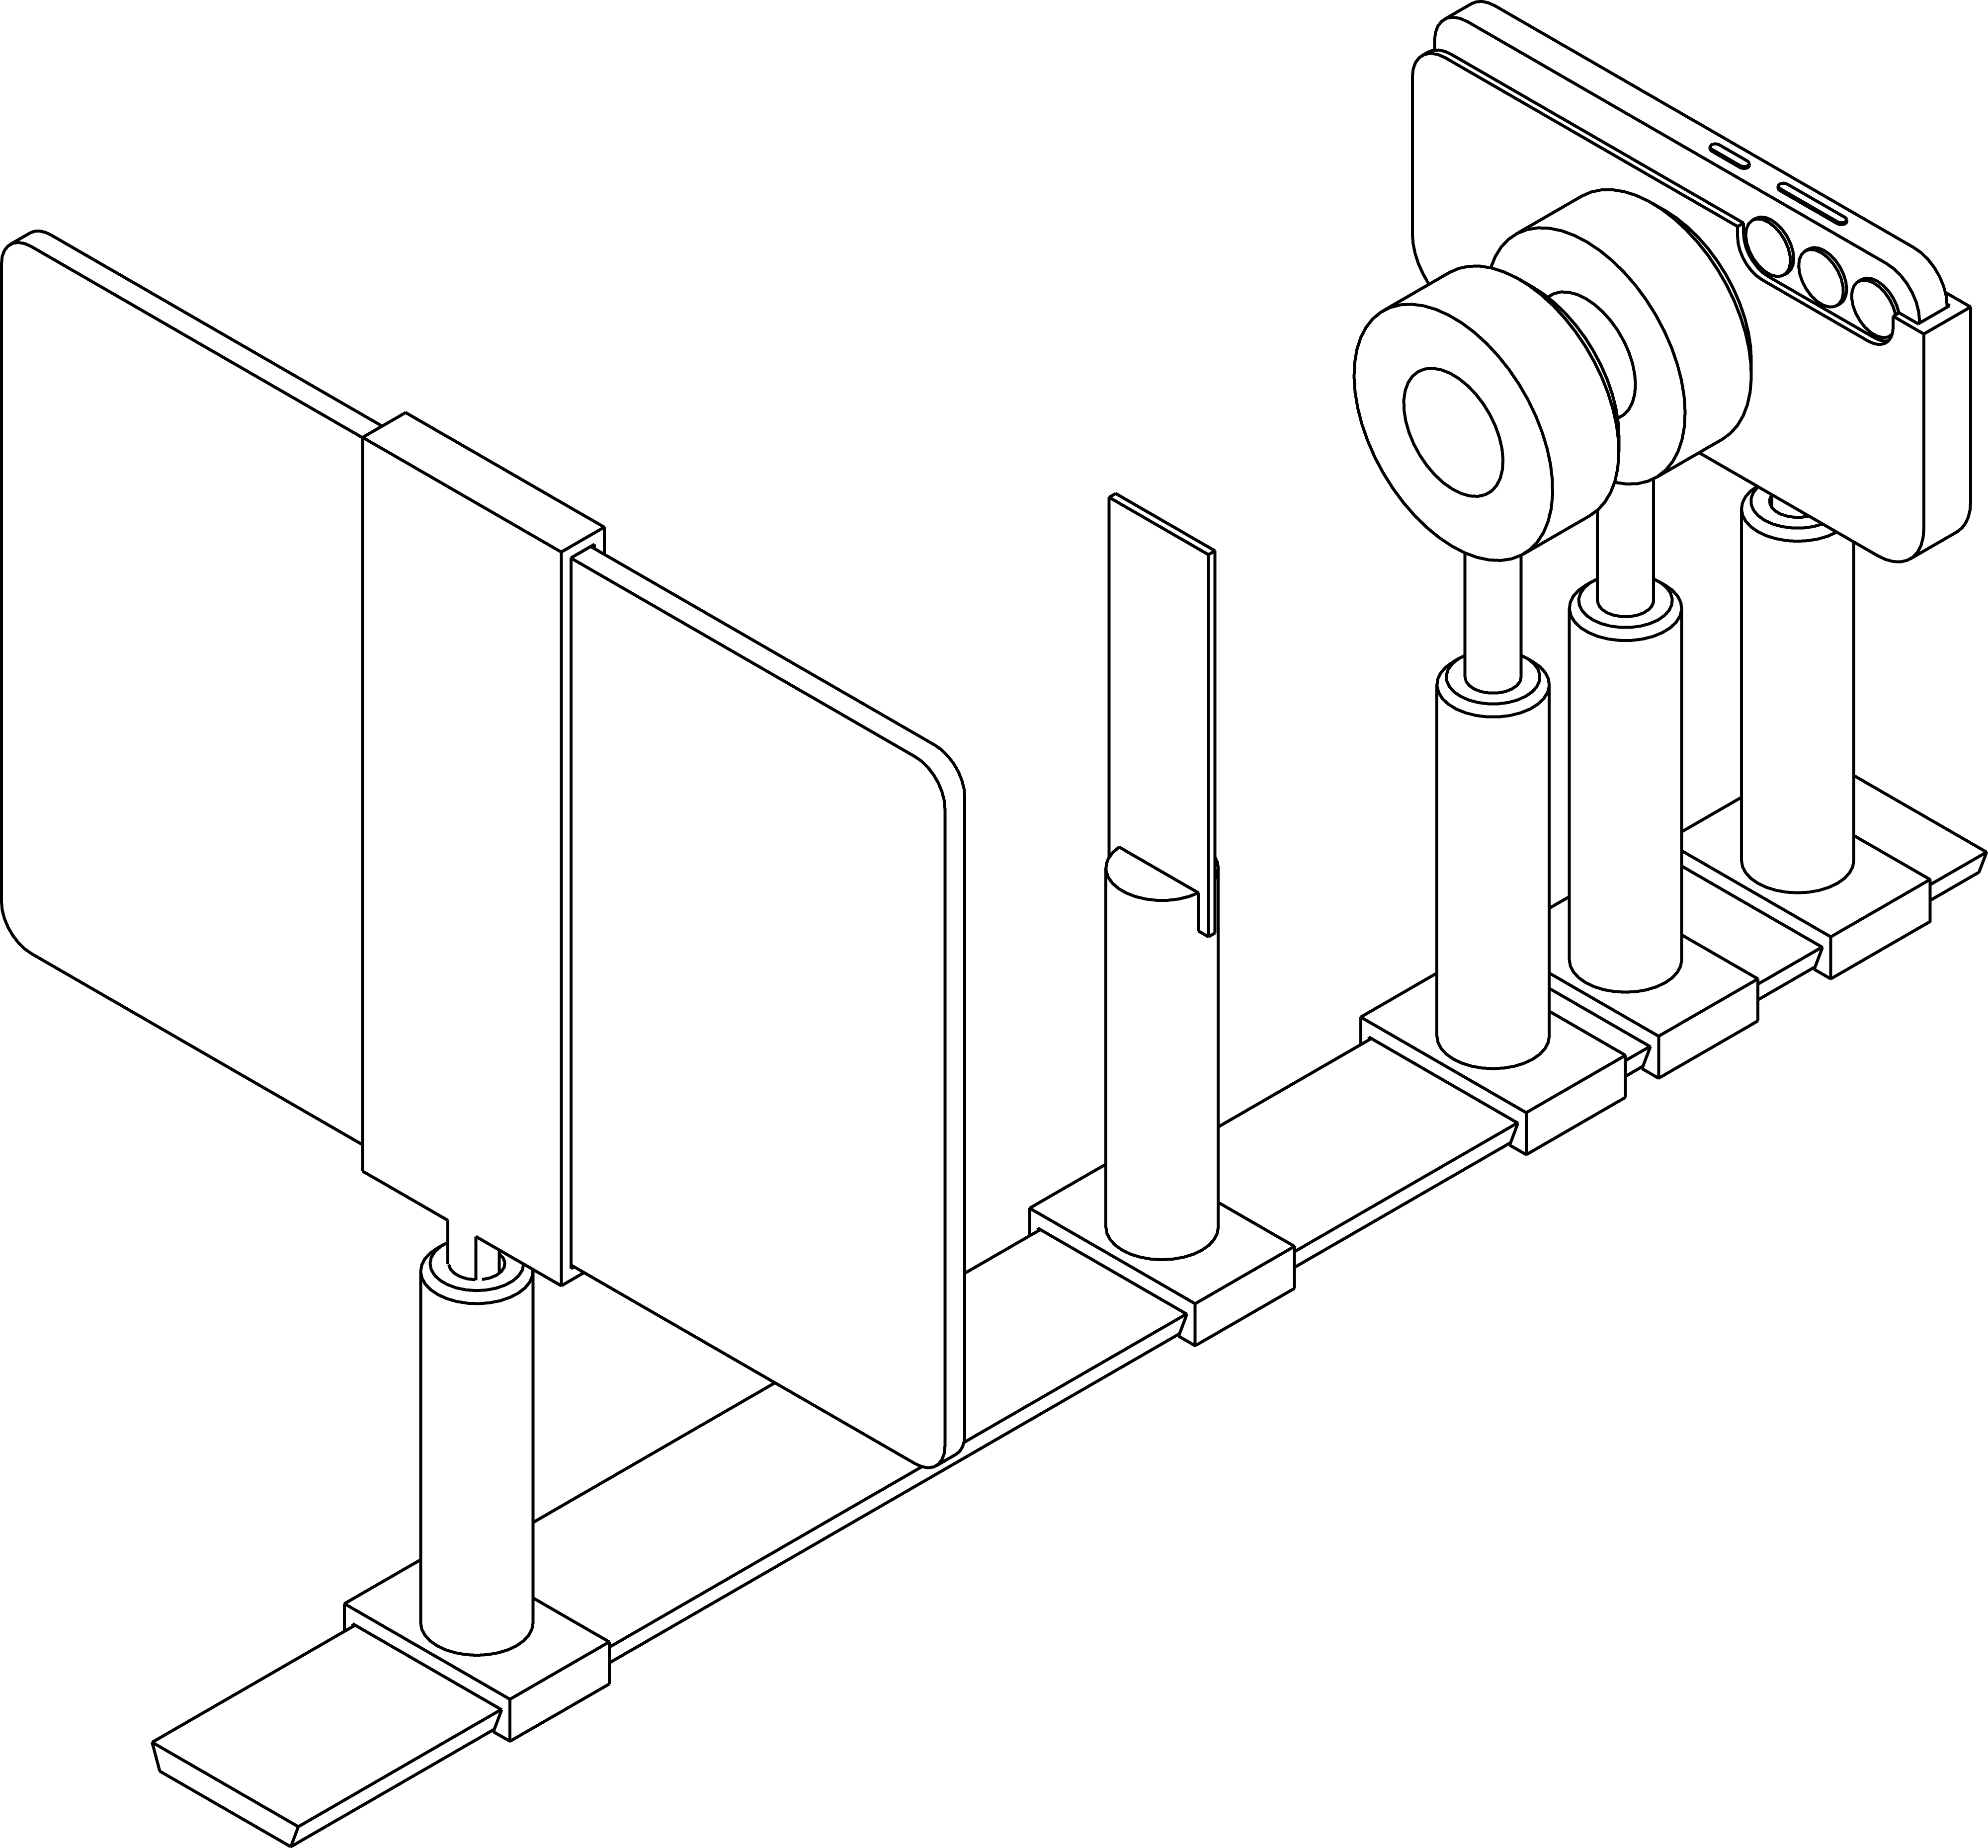
\includegraphics[width=0.48\textwidth]{Images/setup/vista_NE.png}\label{fig:vista_NE}}
    \hfill
    \subfloat[Vista da sensore a sorgente]{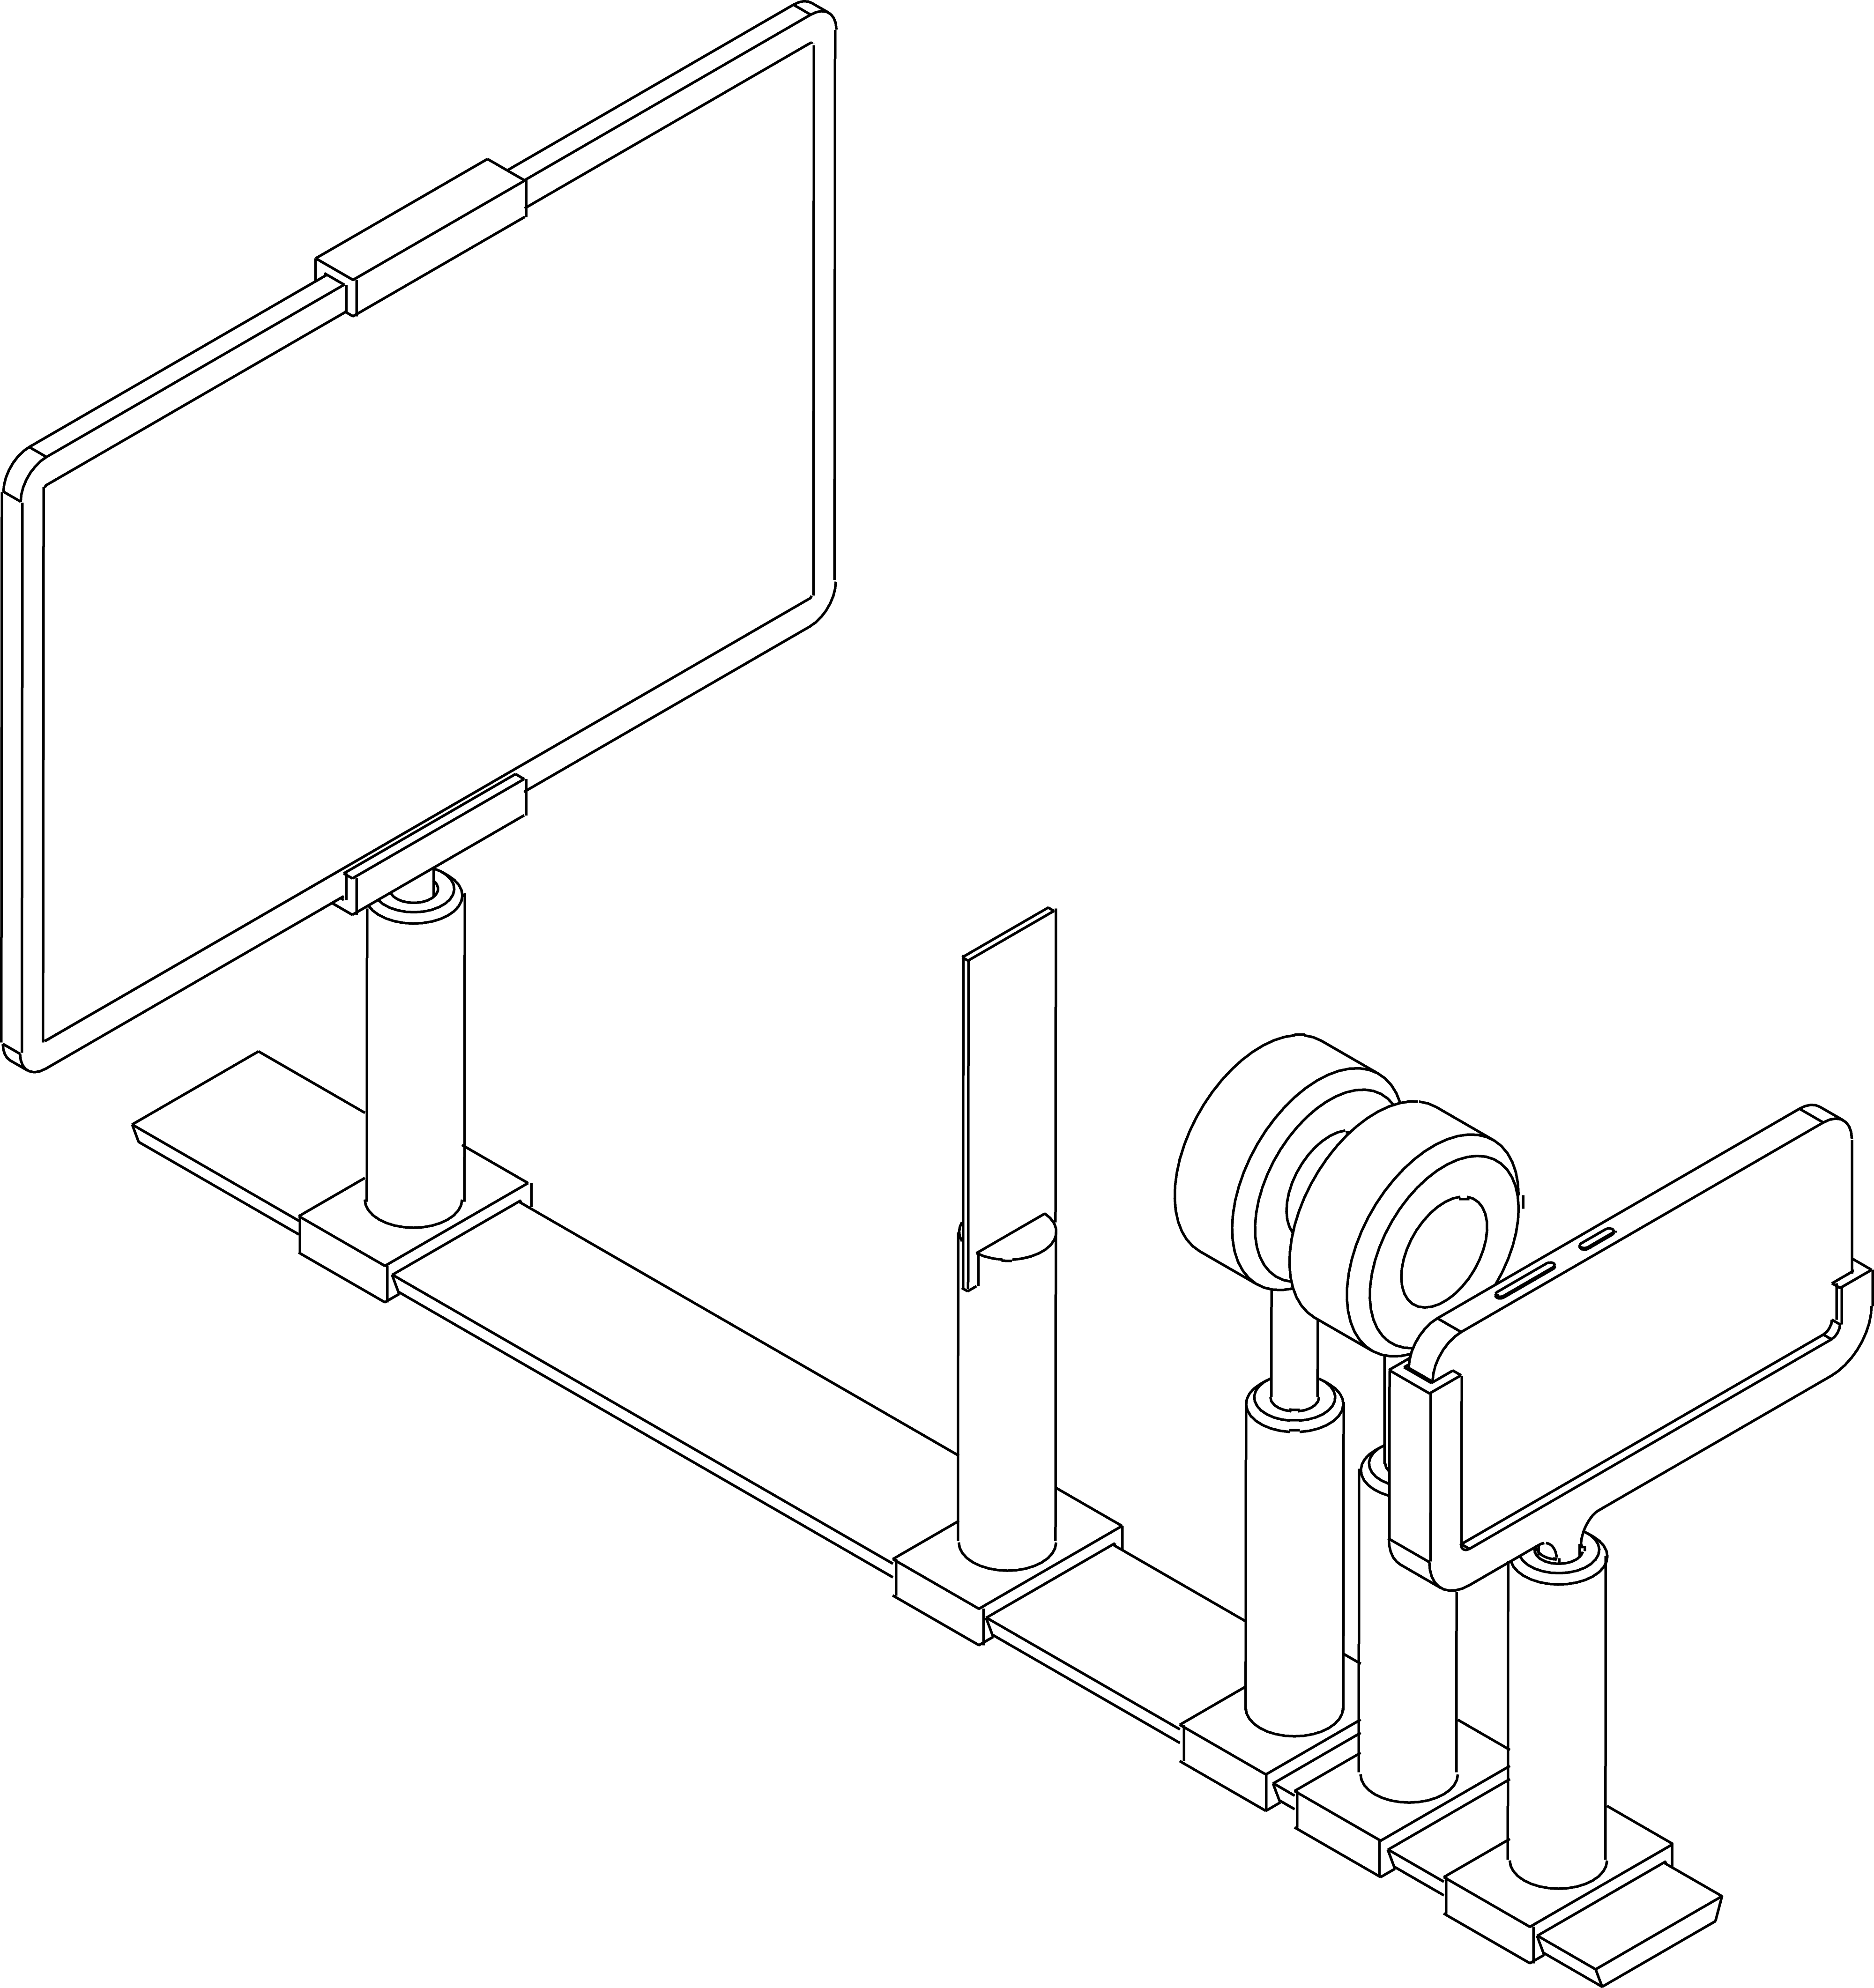
\includegraphics[width=0.48\textwidth]{Images/setup/vista_NW.png}\label{fig:vista_NW}}
    \caption{Fotografie dell'apparato sperimentale assemblato sulla rotaia ottica Optosci.}
    \label{fig:setup-foto}
\end{figure}


\section{Componenti ottici}
\label{sec:componenti-ottici}

L'apparato è montato su una rotaia ottica Optosci con cavalieri scorrevoli, che garantisce l'allineamento dei componenti lungo un asse ottico comune e la riproducibilità del posizionamento tra sessioni di misura. La sorgente luminosa è il display di un tablet Samsung Galaxy Tab S7 FE, impostato su schermata bianca alla massima luminosità. Il pannello LCD emette luce bianca a banda larga attraverso un polarizzatore integrato: la luce in uscita è già polarizzata linearmente con asse orientato approssimativamente in verticale in configurazione landscape, il che rende il display una sorgente estesa a stato di polarizzazione ben definito. L'analizzatore è un polarizzatore lineare Optosci di forma circolare, montato su supporto rotante calibrato con risoluzione angolare sufficiente per i passi di \SI{10}{\degree} previsti dal protocollo; un rapporto di estinzione elevato garantisce che la modulazione dell'intensità trasmessa segua fedelmente la legge di Malus. Per integrare i dispositivi nella rotaia sono stati realizzati supporti personalizzati mediante stampa 3D in PLA.

\subsection{Lamina \texorpdfstring{$\lambda/4$}{lambda/4} zero-order}
\label{subsec:lamina-qwp}

Per la determinazione del parametro $S_3$ viene utilizzata una lamina quarto d'onda Optosci di tipo \emph{zero-order}, progettata per la lunghezza d'onda di $\SI{633}{\nano\meter}$. Il materiale birifrangente della lamina non è dichiarato dal costruttore e resta ignoto: nelle analisi spettrali che seguono il quarzo cristallino compare unicamente come modello di dispersione di riferimento, ben caratterizzato in letteratura, e non come materiale accertato delle lamine. Rispetto a una lamina multi-ordine, la dipendenza dalla lunghezza d'onda è più debole, proprietà importante dato che il sensore opera simultaneamente sui tre canali colore. Il ritardo effettivo alla lunghezza d'onda $\lambda$ del canale in esame è:
\begin{equation}
\delta(\lambda) = \frac{\pi}{2} \cdot \frac{\SI{633}{\nano\meter}}{\lambda}
\label{eq:qwp-geometrico}
\end{equation}
La correzione per questo effetto cromatico è descritta nel \cref{ch:analisi}.


\section{Sensore e acquisizione RAW}
\label{sec:sensore}

Il rivelatore è la fotocamera principale di uno smartphone Samsung Galaxy S24, con sensore CMOS da circa 10 megapixel effettivi, obiettivo a focale $\SI{7.0}{\milli\meter}$ (equivalente $\SI{69}{\milli\meter}$), apertura $f/2.4$ e profondità di acquisizione fino a 12~bit per canale.

% TODO: check (figura Bayer da Wikimedia Commons inserita da AI 2026-05-21, lic. CC BY-SA 3.0)
Il sensore è ricoperto da una matrice di Bayer con disposizione RGGB (\cref{fig:bayer}). In condizioni normali di utilizzo, il processore di immagini dello smartphone applicherebbe demosaicizzazione, bilanciamento del bianco, correzione della gamma e compressione, elaborazioni che distruggono la linearità del segnale. Per questo motivo, tutte le acquisizioni sono effettuate in formato RAW (DNG, \emph{Digital Negative}), che fornisce il segnale grezzo a 12~bit con risposta proporzionale all'intensità incidente, condizione necessaria per l'applicazione della legge di Malus. La dinamica di $2^{12} = 4096$ livelli per canale garantisce una risoluzione sufficiente per distinguere variazioni sottili nell'intensità polarizzata, e ciascun canale colore (R, G, B) può essere estratto e analizzato indipendentemente, consentendo di fatto un'analisi polarimetrica a tre lunghezze d'onda con un singolo sensore. L'acquisizione viene controllata da remoto via USB tramite il software \texttt{scrcpy}, per evitare vibrazioni indotte dal contatto con il dispositivo.

\begin{figure}[H]
    \centering
    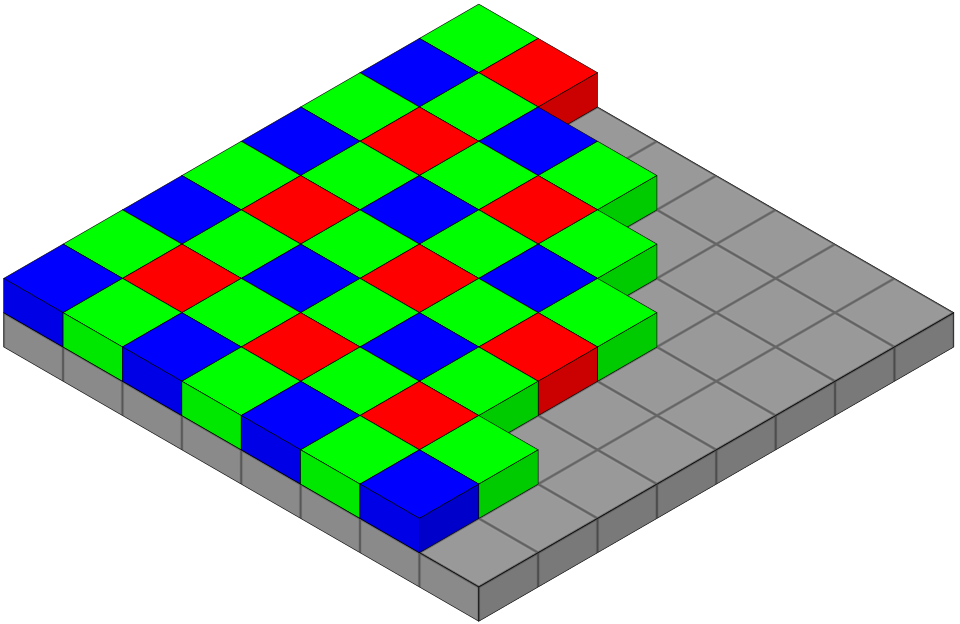
\includegraphics[width=0.45\textwidth]{Images/bayer_pattern.png}
    \caption{Disposizione della matrice di filtri di Bayer in configurazione RGGB: ogni cella di $2\times2$ fotositi comprende un filtro rosso, uno blu e due verdi. Estraendo dal RAW solo i fotositi di un dato colore si ottiene una mappa di intensità per quel canale, alla base dell'analisi polarimetrica a tre lunghezze d'onda. Immagine di Cburnett (Wikimedia Commons), licenza CC BY-SA 3.0.}
    \label{fig:bayer}
\end{figure}


\section{Protocollo di acquisizione}
\label{sec:protocollo}

\subsection{Acquisizione per i parametri di Stokes lineari (\texorpdfstring{$S_0$, $S_1$, $S_2$}{S0, S1, S2})}
\label{subsec:acquisizione-lineari}

La determinazione dei parametri di Stokes lineari $S_0$, $S_1$ e $S_2$ si basa sull'acquisizione di una sequenza di 36 immagini RAW, corrispondenti a 36 posizioni angolari dell'analizzatore distribuite uniformemente tra \SI{0}{\degree} e \SI{350}{\degree} con passo di \SI{10}{\degree}. Con 36 misure per 3 incognite, il sistema è fortemente sovradeterminato: i parametri di Stokes vengono estratti mediante la matrice pseudo-inversa di Moore-Penrose, come descritto nel \cref{ch:analisi}. La sovradeterminazione migliora la robustezza statistica del fit, riducendo l'effetto del rumore del sensore. Gli angoli nominali dell'analizzatore entrano direttamente nella ricostruzione; l'orientazione del sistema di riferimento polarimetrico viene fissata a valle, allineando gli assi alla direzione di polarizzazione del display (\cref{ch:analisi}), mentre la convenzione di elicità è ancorata al segno di $S_3$ (\cref{ch:teoria}).

\subsection{Acquisizione per il parametro di Stokes circolare (\texorpdfstring{$S_3$}{S3})}
\label{subsec:acquisizione-s3}
% TODO: check (cite manuale aggiunta da AI 2026-05-21)
Per la determinazione di $S_3$, secondo il metodo descritto nel manuale di laboratorio del corso di Fisica Sperimentale del Politecnico di Milano~\cite{manuale_polarizzazione}, si acquisiscono due immagini aggiuntive inserendo la lamina $\lambda/4$ nel percorso ottico tra il campione e l'analizzatore: una con l'asse veloce orientato a $+45^\circ$ rispetto all'asse dell'analizzatore, e una a $-45^\circ$. Il parametro $S_3$ viene calcolato dalla differenza delle intensità misurate nelle due configurazioni, con la correzione per la dispersione cromatica della lamina descritta nella \cref{subsec:lamina-qwp}; l'ordine delle due immagini nella differenza fissa il segno di $S_3$ secondo la convenzione di elicità adottata (\cref{sec:determinazione-s3}).

Tutti i parametri di esposizione vengono fissati manualmente e mantenuti costanti per l'intera sessione (\cref{tab:costanti-radiometriche}). Le acquisizioni avvengono in oscurità ambientale, con la sola illuminazione del display del tablet, per eliminare contributi di luce parassita. I parametri di Stokes normalizzati ($s_i = S_i/S_0$) sono per definizione indipendenti dall'intensità assoluta della sorgente, eliminando la necessità di una calibrazione assoluta; la variabilità residua è dominata dal rumore del sensore, ridotto dal downsampling e dalla sovradeterminazione del sistema lineare.

\begin{table}[H]
    \centering
    \caption{Costanti radiometriche impostate durante l'acquisizione.}
    \label{tab:costanti-radiometriche}
    \begin{tabular}{ll}
        \hline
        \textbf{Parametro} & \textbf{Valore} \\
        \hline
        Formato di acquisizione & DNG (Linear RAW, 12~bit/canale) \\
        Lunghezza focale & $\SI{7.0}{\milli\meter}$ ($\SI{69}{\milli\meter}$ eq.\ 35~mm) \\
        Apertura & $f/2.4$ (fissa) \\
        Tempo di esposizione & $1/\SI{90}{\second}$ \\
        Sensibilità ISO & 50 \\
        Bilanciamento del bianco & D65 / Standard Illuminant A \\
        \hline
    \end{tabular}
\end{table}

Il protocollo produce, per ogni sessione di misura, un dataset di 38 immagini RAW: 36 per la ricostruzione dei parametri di Stokes lineari e 2 per il parametro circolare. Il capitolo seguente presenta i campioni selezionati per la validazione dell'apparato, scelti per coprire i tre fenomeni polarimetrici descritti nel \cref{ch:teoria}.

\REVend{revSetup}

\chapter{Campioni}
\label{ch:campioni}
\REVstart{revSetup}
% Capitolo 4: Campioni

I campioni sono stati scelti per coprire i tre fenomeni polarimetrici di interesse (birifrangenza, attività ottica e fotoelasticità), scegliendo materiali trasparenti compatibili con la configurazione in trasmissione. Alcuni possiedono parametri nominali noti, utili per una validazione quantitativa; altri offrono strutture spaziali che mettono alla prova la capacità di imaging del sistema. La \cref{tab:campioni} ne riassume le caratteristiche principali; tutti sono inseriti nel porta-campione sulla rotaia, tra sorgente e analizzatore, e le superfici vengono pulite prima dell'acquisizione.

\begin{table}[H]
    \centering
    \caption{Campioni analizzati con il polarimetro a immagine.}
    \label{tab:campioni}
    \small
    \begin{tabularx}{\textwidth}{@{}l >{\raggedright\arraybackslash}X >{\raggedright\arraybackslash}X@{}}
        \hline
        \textbf{Campione} & \textbf{Fenomeno} & \textbf{Validazione attesa} \\
        \hline
        Lamina $\lambda/2$  & Birifrangenza & $\delta \approx 180^\circ$, AoLP ruotato \\
        Lamina $\lambda/4$ & Birifrangenza & $|S_3/S_0|$ massimo \\
        Nastro adesivo (1--5 strati) & Birifrangenza incrementale & $\delta \propto N$ \\
        Soluzione di saccarosio & Attività ottica & $\alpha_\text{rot} \propto 1/\lambda^2$ \\
        Righello in plastica & Fotoelasticità (stress residuo) & Frange isocromatiche \\
        Trave a sbalzo & Fotoelasticità (stress applicato) & Birifrangenza indotta dal carico \\ % TODO: check (cella modificata da AI 2026-05-21)
        \hline
    \end{tabularx}
\end{table}


\section{Campioni birifrangenti}
\label{sec:campioni-birifrangenti}

Le lamine d'onda commerciali ($\lambda/2$ e $\lambda/4$, lunghezza d'onda di design di $\SI{633}{\nano\meter}$, cfr.\ \cref{sec:fenomeni}) sono il primo test di validazione quantitativa: la ritardanza nominale è specificata dal costruttore e la risposta è spazialmente uniforme, il che consente un confronto diretto tra valore misurato e valore atteso. La lamina $\lambda/4$, orientata a $\SI{45}{\degree}$ rispetto alla polarizzazione incidente, produce luce circolarmente polarizzata con $|S_3/S_0| \approx 1$; la lamina $\lambda/2$ ruota il piano di polarizzazione di un angolo pari al doppio della sua orientazione, con ritardanza nominale $\delta \approx 180^\circ$. L'ordine delle due lamine non è dichiarato dal costruttore, sicché a priori se ne conosce soltanto la ritardanza nominale alla lunghezza d'onda di design: l'analisi del \cref{ch:risultati} le caratterizzerà a posteriori, mostrando che la $\lambda/4$ è compatibile con un ritardatore a singolo ordine, mentre la $\lambda/2$ si rivelerà multi-ordine, circostanza che ne fa un caso di studio sull'ambiguità di avvolgimento anziché un semplice riferimento di ritardanza nota.

Il vetrino con strati di nastro adesivo trasparente (da 1 a 5 strati, in configurazione simmetrica $1$-$2$-$3$-$4$-$5$-$4$-$3$-$2$-$1$) è un campione a birifrangenza incrementale controllata: % TODO: check (spiegazione birifrangenza nastro inserita da AI 2026-05-21)
il film polimerico del nastro, stirato uniassialmente in fase di produzione, ha le catene molecolari allineate lungo una direzione preferenziale, e questa anisotropia strutturale gli conferisce una birifrangenza intrinseca. La ritardanza totale cresce approssimativamente come
\begin{equation}
\delta_{\text{tot}} \approx N \cdot \delta_{\text{singolo}},
\label{eq:ritardo-strati}
\end{equation}
dove $N$ è il numero di strati e $\delta_{\text{singolo}}$ il ritardo introdotto da un singolo strato. La simmetria del campione fornisce un controllo interno di consistenza: le regioni con lo stesso numero di strati ai due lati del vetrino devono restituire ritardanze concordanti.


\section{Attività ottica}
\label{sec:campione-attivita-ottica}

Una soluzione di saccarosio (in una boccetta con cammino ottico $l = \SI{13}{\milli\meter}$) consente di verificare due aspetti: la rotazione uniforme del piano di polarizzazione, osservabile come variazione dell'AoLP, e la legge di dispersione $\alpha_\text{rot} \propto 1/\lambda^2$ (modello di Drude), sfruttando i tre canali colore del sensore. Il saccarosio destrogiro ha rotazione specifica $[\alpha]_D = \SI{66.47}{\degree\per(\deci\meter\cdot\gram\per\milli\liter)}$ alla riga D del sodio.


\section{Campioni fotoelastici}
\label{sec:campioni-fotoelastici}

Un righello in plastica trasparente presenta tensioni residue da stampaggio a iniezione che generano birifrangenza non uniforme nel materiale. Quando posto tra polarizzatore e analizzatore, le regioni a diverso stato di tensione producono le frange isocromatiche e isocline tipiche dei materiali fotoelastici (cfr.\ \cref{sec:fenomeni}). L'analisi con il polarimetro a immagine consente di mappare spazialmente la distribuzione delle tensioni interne.

Una trave in materiale trasparente, vincolata a un'estremità, è stata analizzata in due condizioni: scarica, per verificare l'eventuale presenza di tensioni residue, e sotto carico, con un peso applicato all'estremità libera. % TODO: check (paragrafo trave riscritto da AI 2026-05-21: frange -> variazione birifrangenza, qualitativo)
Lo sforzo di flessione varia linearmente lungo lo spessore e inversamente con la distanza dal vincolo, inducendo per effetto fotoelastico una birifrangenza non uniforme lungo la trave. Nelle condizioni di questo esperimento le frange isocromatiche non risultano nettamente risolte: si osserva piuttosto una variazione delle proprietà di birifrangenza, rilevabile soprattutto come modulazione di $S_3$ fra trave carica e scarica. L'analisi su questo campione resta perciò qualitativa.
\REVend{revSetup}

\chapter{Analisi dei dati}
\label{ch:analisi}
\REVstart{revAnalisi}
% Capitolo 5: Analisi dei dati

Le 38 immagini RAW acquisite per ogni campione vengono elaborate in sequenza per ricavare i parametri di Stokes e le grandezze polarimetriche derivate. L'intera catena di analisi è stata implementata in Python, sfruttando le librerie \texttt{numpy}, \texttt{rawpy}, \texttt{scipy} e \texttt{scikit-image} per le operazioni di morfologia e di rivelazione dei bordi.

% ---------------------------------------------------------------------------
\section{Dalla immagine grezza alla matrice di intensità}
\label{sec:preelaborazione}

Per ciascun file DNG si accede direttamente al piano di Bayer del sensore, senza demosaicizzazione né bilanciamento del bianco: dei quattro fotositi del super-pixel di Bayer si estrae quello associato al canale colore di interesse, ottenendo un array bidimensionale in virgola mobile a singola precisione con risoluzione pari a metà di quella nativa del sensore lungo entrambi gli assi. Questa scelta evita la diafonia cromatica introdotta dalla matrice di colore della fotocamera nei flussi di demosaicizzazione standard, preservando la proporzionalità lineare tra il valore numerico letto e il numero di fotoelettroni raccolti dal singolo fotosito. Sul medesimo piano vengono applicate due correzioni preliminari, descritte di seguito, prima dell'eventuale riduzione di risoluzione spaziale.

\subsection{Sottrazione del frame oscuro}
\label{subsec:dark_frame}

Il sensore CMOS presenta un piedistallo di lettura non nullo anche in assenza di luce, somma del rumore di lettura e della corrente di buio dei fotositi. Per stimarlo si acquisisce un frame con l'obiettivo coperto al medesimo tempo di esposizione utilizzato per le misure polarimetriche, e lo si sottrae a ciascuna delle 38 immagini grezze. La sottrazione viene eseguita alla risoluzione nativa del sensore, prima di qualsiasi operazione di riduzione spaziale, perché il piedistallo è una proprietà locale del singolo fotosito e si propagherebbe in maniera non lineare attraverso una media a blocchi. Il frame oscuro è caricato una sola volta dalla pipeline e mantenuto in cache fra le 38 chiamate per minimizzare il costo di lettura.

\subsection{Mascheramento dei pixel saturi}
\label{subsec:saturazione}

Quando un fotosito raggiunge il livello di bianco dichiarato nei metadati del file DNG, pari a $4095$~conteggi per la lettura lineare a $12$~bit, la risposta del sensore tronca l'andamento sinusoidale della legge di Malus. I pixel saturi, se inclusi nella ricostruzione ai minimi quadrati, distorcono sistematicamente i parametri $S_0$, $S_1$ e $S_2$ ricavati, in misura proporzionale alla frazione di angoli per i quali la saturazione si verifica. Si adotta una soglia conservativa al $98\%$ del livello di bianco, corrispondente a circa $4013$~conteggi, e si costruisce un accumulatore booleano alla risoluzione nativa del sensore che traccia, in disgiunzione logica su tutte le 38 immagini, ogni fotosito che almeno una volta abbia superato la soglia. L'accumulatore viene poi ricampionato sulla griglia di analisi e i pixel coinvolti vengono marcati come non disponibili (\texttt{NaN}) nelle mappe finali dei parametri di Stokes. La conservazione dell'informazione di saturazione alla risoluzione nativa è essenziale: un singolo fotosito clippato all'interno di un blocco $f \times f$ comprometterebbe il valor medio del blocco, e una soglia stabilita dopo il downsampling non sarebbe in grado di rilevarlo.

\subsection{Riduzione della risoluzione spaziale}
\label{subsec:downsampling}

Le immagini del sensore hanno una risoluzione nativa dell'ordine di $4000 \times 3000$~pixel. Poiché l'elaborazione richiede lo stack simultaneo di 38 immagini, si applica un downsampling con fattore $f$ configurabile: l'immagine, già corretta dal frame oscuro, viene suddivisa in blocchi non sovrapposti di $f \times f$~pixel, ciascuno sostituito dal valor medio delle intensità contenute. Valori tipici sono $f = 4$--$20$, corrispondenti a risoluzioni risultanti comprese tra $1000 \times 750$ e $200 \times 150$~pixel. Il compromesso introdotto è la perdita di dettagli spaziali fini, irrilevante per i campioni macroscopici analizzati in questo lavoro.

% ---------------------------------------------------------------------------
\section{Lunghezze d'onda effettive dei canali colore}
\label{sec:centroide}

Il sensore CMOS non è un rivelatore monocromatico: ciascun canale colore ha una risposta spettrale estesa su diverse decine di nanometri. Poiché la ritardanza introdotta dalla lamina quarto d'onda dipende dalla lunghezza d'onda (\cref{sec:determinazione-s3}), è necessario assegnare a ciascun canale una lunghezza d'onda effettiva rappresentativa.

% TODO: Approfondire come abbiamo lo spettro, così sembra piovuto dal cielo, misurato tramite AvaSpec 2048
Il metodo adottato è il baricentro con soglia. Dati lo spettro di emissione della sorgente $I(\lambda)$ e la sensibilità spettrale del canale $S_c(\lambda)$, il segnale effettivo registrato è $E_c(\lambda) = S_c(\lambda) \cdot I(\lambda)$. La lunghezza d'onda centroide si calcola come media pesata, dopo aver applicato una soglia al $30\%$ del valore di picco per escludere le code a bassa intensità:
\begin{equation}
    \lambda_{\mathrm{eff},c} = \frac{\displaystyle\sum_{\lambda:\,E_c(\lambda) \geq 0.3\,E_c^{\max}} \lambda \cdot E_c(\lambda)}{\displaystyle\sum_{\lambda:\,E_c(\lambda) \geq 0.3\,E_c^{\max}} E_c(\lambda)}.
    \label{eq:centroide}
\end{equation}
I dati di sensibilità spettrale utilizzati sono quelli del Samsung Galaxy S22 Rear Telephoto, adottato come proxy per il sensore del Galaxy S24 per l'obiettivo telephoto, ottenuti dal database pubblico Color Lab Eilat~\cite{Solomatov2023spectral}. Lo spettro della sorgente LCD è stato misurato separatamente.

% ---------------------------------------------------------------------------
\section{Ricostruzione di \texorpdfstring{$S_0$, $S_1$, $S_2$}{S0, S1, S2}}
\label{sec:stokes_lineari}

L'intensità trasmessa da un analizzatore lineare orientato ad angolo $\theta$ rispetto all'asse di riferimento segue la legge di Malus generalizzata (\cref{eq:malus_generalizzata}):
\begin{equation}
    I(\theta) = \frac{1}{2}\bigl(S_0 + S_1 \cos 2\theta + S_2 \sin 2\theta\bigr).
    \label{eq:malus_generalizzata_analisi}
\end{equation}
Per ogni pixel, le intensità misurate ai 36 angoli equispaziati $\theta_i = 0^\circ, 10^\circ, \ldots, 350^\circ$ costituiscono un sistema di 36 equazioni in 3 incognite. In forma matriciale $\mathbf{I} = \mathbf{A}\,\mathbf{p}$, dove $\mathbf{p} = [S_0/2,\; S_1/2,\; S_2/2]^T$ e la matrice del sistema ha righe $[1,\; \cos 2\theta_i,\; \sin 2\theta_i]$. La soluzione ai minimi quadrati si ottiene tramite la pseudo-inversa di Moore-Penrose:
\begin{equation}
    \mathbf{p} = (\mathbf{A}^T \mathbf{A})^{-1} \mathbf{A}^T \, \mathbf{I}.
    \label{eq:pseudoinversa}
\end{equation}
Poiché la matrice $\mathbf{A}$ non dipende dal pixel, la pseudo-inversa viene calcolata una sola volta e applicata all'intero stack di immagini con un singolo prodotto matriciale, restituendo le tre mappe $S_0$, $S_1$, $S_2$. Gli angoli nominali dell'analizzatore vengono invertiti ($\theta = 360^\circ - \theta_{\mathrm{nom}}$) per garantire coerenza con la convenzione destrorsa del formalismo di Stokes.

% ---------------------------------------------------------------------------
\section{Determinazione della componente circolare \texorpdfstring{$S_3$}{S3}}
\label{sec:determinazione-s3}
Il parametro $S_3$, che quantifica la componente di polarizzazione circolare, non è accessibile tramite il solo analizzatore lineare. La sua misura richiede l'inserimento della lamina $\lambda/4$ nel cammino ottico, che converte la polarizzazione circolare in polarizzazione lineare analizzabile. Le due immagini acquisite con la lamina a $+45^\circ$ e $-45^\circ$ forniscono le intensità $I_{+45}$ e $I_{-45}$, legate a $S_3$ dalla relazione~\cite{manuale_polarizzazione}:
\begin{equation}
    S_3 = \frac{I_{+45} - I_{-45}}{\sin\delta(\lambda)},
    \label{eq:s3_formula}
\end{equation}
dove $\delta(\lambda)$ è il ritardo di fase effettivo della lamina alla lunghezza d'onda di lavoro, calcolato secondo la \cref{eq:dispersione-qwp}. Anche l'orientazione della lamina viene invertita per coerenza con la convenzione destrorsa. Il fattore correttivo $1/\sin\delta(\lambda)$ compensa la dipendenza cromatica della lamina zero-order; per il canale rosso ($\lambda_{\mathrm{eff}} \approx \SI{600}{\nano\meter}$) il fattore è circa $1.05$, modesto ma non trascurabile per misure quantitative.

% ---------------------------------------------------------------------------
\section{Segmentazione della regione di sfondo}
\label{sec:mascheramento}

Solo una porzione del campo visivo è effettivamente attraversata dal fascio polarimetrico utile. Le regioni occupate dal campione e dal suo supporto vanno separate dallo sfondo libero, poiché quest'ultimo costituisce il riferimento sperimentale dello stato di polarizzazione in ingresso ed entra direttamente nei fit di calibrazione descritti nelle sezioni successive. Una contaminazione anche parziale dello sfondo con pixel di campione propaga errori sistematici alle correzioni di rotazione del sistema di riferimento e di ribasamento della sfera di Poincaré, e da queste all'intera mappa di ritardanza. Per questo motivo la maschera binaria che identifica lo sfondo è generata da una procedura conservativa, calibrata per sopportare le geometrie eterogenee dei campioni considerati senza richiedere parametri specifici di volta in volta.

La maschera si costruisce a partire dalla sola mappa di intensità $S_0$, attraverso una catena di operazioni morfologiche e di segmentazione progettata per essere invariante rispetto alla risoluzione di lavoro: tutti i raggi degli elementi strutturanti sono espressi come frazioni del lato maggiore dell'immagine, oppure come quantità in pixel nativi riscalate per il fattore di downsampling $f$. Dapprima si normalizza $S_0$ nell'intervallo $[0, 1]$ tramite riscalamento min-max. Una soglia di scurità al $30\%$ del massimo classifica come appartenenti al campione tutti i pixel sufficientemente scuri, intercettando per via diretta supporti opachi e montature anche dove il contrasto con lo sfondo è ridotto. In parallelo, il rivelatore di bordi di Canny~\cite{Canny1986} con deviazione gaussiana% TODO: verificare/aggiungere voce BibTeX Canny1986 (J.~Canny, IEEE TPAMI 8(6):679--698, 1986, DOI:10.1109/TPAMI.1986.4767851) $\sigma = 1{,}5$~px e soglie isteretiche assolute $T_{\mathrm{low}} = 0{,}05$ e $T_{\mathrm{high}} = 0{,}15$ sull'ampiezza del gradiente individua le discontinuità di intensità che delimitano il campione. I bordi rilevati vengono dilatati con un elemento strutturante a disco di raggio pari a circa lo $0{,}4\%$ del lato maggiore dell'immagine, in modo da fondere segmenti vicini ma non perfettamente allineati in una barriera continua. L'unione fra bordi dilatati e prior di scurità definisce la barriera ostruttiva, sulla quale si applica una chiusura morfologica di raggio dimezzato per cucire eventuali interruzioni residue.

Lo sfondo si identifica come il complemento di tale barriera mediante una procedura di \emph{flood fill} dal bordo dell'immagine. Si etichettano le componenti connesse del complemento, si selezionano quelle che toccano almeno un lato dell'immagine e si conservano nell'unione tutte le componenti la cui area è pari ad almeno il $20\%$ di quella della componente bordo-tangente di area massima. La logica multi-componente è essenziale per campioni verticali estesi che attraversano l'intero campo di vista, come la bottiglia del campione di soluzione zuccherina, i quali dividerebbero altrimenti lo sfondo legittimo in due regioni disgiunte; al contempo, la soglia del $20\%$ esclude piccoli inganni dovuti a fughe interne al campione associate a bordi di Canny incompleti. La maschera del campione si ottiene per complemento, riempiendone le eventuali cavità interne con un'operazione di \texttt{binary\_fill\_holes} per assorbire residui di sfondo intrappolati nel campione, seguita da un'apertura morfologica con disco di piccolo raggio per regolarizzare il contorno.

Per intercettare segmentazioni anomale prima che inquinino le statistiche di sfondo, si valuta la compattezza geometrica $\kappa = 4\pi A / P^2$ della componente di campione di area massima, dove $A$ è l'area e $P$ il perimetro misurato come dilatazione a 4-connessione meno la maschera stessa. Forme regolari prossime al cerchio danno $\kappa \to 1$, mentre contorni frastagliati abbassano $\kappa$ sotto $0{,}05$, valore che attiva un avviso esplicito di segmentazione probabilmente compromessa. Infine la maschera di sfondo viene erosa con un disco di raggio scalato come $100/f$ pixel ricampionati, equivalente a $100$~pixel nella risoluzione nativa, per garantire un margine di sicurezza dalla frontiera del campione. Se a valle del procedimento la frazione di pixel di sfondo risulta degenere (inferiore all'$1\%$ o superiore al $99{,}5\%$ del campo) la pipeline ricorre a un fallback basato sulla sola soglia di intensità, segnalando l'evento nel log di esecuzione.

% ---------------------------------------------------------------------------
\section{Allineamento del sistema di riferimento}
\label{sec:allineamento}

L'asse di polarizzazione di uscita del display LCD non è perfettamente allineato con l'asse di riferimento dell'analizzatore. Questo offset angolare si manifesta come una rotazione sistematica delle mappe di $S_1$ e $S_2$, alla quale si sovrappongono variazioni spaziali lente dovute all'imperfetta uniformità del fascio di illuminazione e alla curvatura residua dei polarizzatori del pannello. Trattare la correzione come una rotazione scalare uniforme — ad esempio adoperando un angolo mediano sullo sfondo — lascia residui non trascurabili, in particolare ai bordi del campo. Si adotta pertanto una rotazione a campo locale, ricavata da un fit indipendente delle superfici di $S_1$ e $S_2$ sulla sola regione di sfondo.

Sui pixel della maschera di sfondo si scrivono $S_1(x, y)$ e $S_2(x, y)$ come polinomi completi di grado due in coordinate normalizzate $(x_n, y_n) \in [-1, 1]^2$, con base $\{1,\; x_n,\; y_n,\; x_n^2,\; x_n y_n,\; y_n^2\}$. I coefficienti si determinano ai minimi quadrati separatamente per le due componenti, e i polinomi così fittati vengono valutati su tutto il dominio $H \times W$, producendo le superfici $\tilde{S}_1(x, y)$ e $\tilde{S}_2(x, y)$. L'angolo di offset spazialmente variabile si ricostruisce quindi tramite
\begin{equation}
    \alpha_{\mathrm{bg}}(x, y) = \frac{1}{2}\,\arctan_2\!\bigl(\tilde{S}_2(x, y),\; \tilde{S}_1(x, y)\bigr).
    \label{eq:angolo_offset}
\end{equation}
La scelta di fittare le componenti cartesiane $S_1$ e $S_2$ in luogo dell'angolo direttamente è dettata dalla discontinuità di $\arctan_2$ in prossimità di $\pm 90^\circ$: un fit dell'angolo ravvolto produrrebbe salti spuri proprio nei casi in cui la polarizzazione di sfondo si trovi vicino alla frontiera di avvolgimento, mentre il fit separato delle due componenti elimina la discontinuità per costruzione. Il grado due offre un compromesso fra cattura della variazione spaziale residua e robustezza al rumore, sufficiente in tutti i campioni considerati grazie alla densità tipica di decine di migliaia di pixel di sfondo.

I parametri $S_1$ e $S_2$ vengono infine ruotati di $-\alpha_{\mathrm{bg}}(x, y)$ tramite la matrice di rotazione nel piano $(S_1, S_2)$:
\begin{equation}
    \begin{pmatrix} S_1' \\ S_2' \end{pmatrix} = \begin{pmatrix} \cos 2\alpha_{\mathrm{bg}} & \sin 2\alpha_{\mathrm{bg}} \\ -\sin 2\alpha_{\mathrm{bg}} & \cos 2\alpha_{\mathrm{bg}} \end{pmatrix} \begin{pmatrix} S_1 \\ S_2 \end{pmatrix}.
    \label{eq:rotazione_stokes}
\end{equation}
Dopo la correzione, la direzione di emissione del display LCD coincide per costruzione con l'asse zero del sistema di riferimento polarimetrico, $S_1' > 0$ e $S_2' \approx 0$ in ogni punto dello sfondo, e tutti gli angoli polarimetrici derivati — AoLP e orientazione dell'asse veloce — sono misurati rispetto ad essa. Formalmente, la trasformazione corrisponde a una rotazione della sfera di Poincaré attorno all'asse $S_3$, e dunque non altera la componente circolare $S_3$ già stimata.

% ---------------------------------------------------------------------------
\section{Correzione dell'ellitticità residua del fascio incidente}
\label{sec:ellitticita}

La rotazione descritta nella \cref{sec:allineamento} azzera la componente $S_2$ dello sfondo ma lascia in generale una componente $S_3$ non nulla. Misure di calibrazione su tutti i campioni rivelano che lo stato di polarizzazione emesso dal display LCD presenta un'ellitticità residua di entità contenuta ma non trascurabile, dovuta alla combinazione di imperfezioni del polarizzatore di uscita del pannello e di micro-birifrangenza degli strati di vetro attraversati dal fascio. Il modello di inversione del ritardatore descritto nella sezione successiva è formulato per uno stato di ingresso puramente lineare con $s_{3,\mathrm{in}} = 0$: una violazione di questa ipotesi propaga un errore al primo ordine in $\beta$, dove $\beta$ è la latitudine dello stato incidente sulla sfera di Poincaré. Per ridurre l'errore residuo al secondo ordine si introduce una seconda rotazione, complementare alla precedente, che porta lo stato di sfondo dall'equatore inclinato all'equatore canonico della sfera.

La rotazione viene effettuata attorno all'asse $S_2$ e agisce nel piano $(S_1, S_3)$:
\begin{equation}
    \begin{pmatrix} S_1'' \\ S_3'' \end{pmatrix} = \begin{pmatrix} \cos\beta(x, y) & \sin\beta(x, y) \\ -\sin\beta(x, y) & \cos\beta(x, y) \end{pmatrix} \begin{pmatrix} S_1' \\ S_3 \end{pmatrix}.
    \label{eq:rotazione_poincare}
\end{equation}
L'angolo $\beta(x, y)$ è ricavato fittando, con la medesima base polinomiale di grado due in coordinate normalizzate adoperata nella \cref{sec:allineamento}, le mappe di $s_{1}$ e $s_{3}$ ristrette alla regione di sfondo, e definendo
\begin{equation}
    \beta(x, y) = \arctan_2\!\bigl(\tilde{s}_{3}(x, y),\; \tilde{s}_{1}(x, y)\bigr).
    \label{eq:beta_poincare}
\end{equation}
La rotazione lascia invariata la componente $S_2$, già allineata, e preserva il modulo del vettore di Stokes per costruzione, conservando di conseguenza il grado di polarizzazione totale. La ritardanza $\delta$ del campione è geometricamente invariante rispetto alla scelta del piano equatoriale: rebasare la sfera di Poincaré non altera l'ampiezza del ritardo introdotto dal campione, ma allinea il modello matematico al riferimento sperimentale.

La maschera utilizzata per il fit di $\beta$ richiede particolare attenzione. La sola maschera di sfondo prodotta dalla \cref{sec:mascheramento} include i pixel scuri associati al supporto e alla montatura della lamina $\lambda/4$, dove la differenza $I_{+45} - I_{-45}$ che entra nella \cref{eq:s3_formula} risulta numericamente degenere. Tali pixel passano i criteri di sfondo basati su $S_0$ ma trasportano un valore di $S_3$ dominato dal rumore. Per escluderli si calcola l'intensità media delle due immagini con lamina, $w(x, y) = \tfrac{1}{2}\bigl[I_{+45}(x, y) + I_{-45}(x, y)\bigr]$, e si definisce una maschera di supporto come l'insieme dei pixel dello sfondo per i quali $w(x, y) < W_{\mathrm{th}}\cdot \max_{\mathrm{bg}} w$, con $W_{\mathrm{th}} = 0{,}50$. A questa si unisce una banda lungo il perimetro dell'immagine, e il risultato viene dilatato con un disco di raggio pari a $150/f$ pixel ricampionati, equivalente a $150$~pixel nella risoluzione nativa, per assorbire la diffrazione di bordo della montatura della lamina. La maschera dedicata al fit di $\beta$ è la differenza fra la maschera di sfondo e quella di supporto così dilatata; un controllo automatico richiede che la maschera risultante conservi almeno il $10\%$ dei pixel di sfondo originali, in difetto del quale la pipeline ricade sulla maschera intera e segnala l'evento.

L'ordine delle operazioni è obbligato dalla geometria della costruzione: si calcolano dapprima i parametri $S_0$, $S_1$ e $S_2$ tramite pseudo-inversa, quindi $S_3$ via lamina $\lambda/4$; si applica l'allineamento del sistema di riferimento sui pixel di sfondo che ribalta $S_1$ e $S_2$, e infine la rotazione di Poincaré qui descritta che ribalta $S_1$ e $S_3$. Le formule di estrazione della ritardanza vengono poi applicate sul terzetto $(S_1'', S_2', S_3'')$, dove sia $\langle S_2 \rangle_{\mathrm{bg}}$ sia $\langle S_3 \rangle_{\mathrm{bg}}$ sono ridotti a zero a meno del fit polinomiale, e l'ipotesi di stato lineare in ingresso è soddisfatta a meno di termini $\mathcal{O}(\beta^2)$.

% ---------------------------------------------------------------------------
\section{Grandezze polarimetriche derivate}
\label{sec:dolp_aolp}

Dai parametri di Stokes allineati si calcolano il grado di polarizzazione lineare (DoLP) e l'angolo di polarizzazione lineare (AoLP):
\begin{equation}
    \mathrm{DoLP} = \frac{\sqrt{S_1'^2 + S_2'^2}}{S_0}, \qquad \mathrm{AoLP} = \frac{1}{2}\arctan\!\left(\frac{S_2'}{S_1'}\right).
    \label{eq:dolp_aolp}
\end{equation}
Il DoLP è limitato all'intervallo $[0, 1]$: valori prossimi a $1$ indicano luce completamente polarizzata linearmente, valori prossimi a $0$ indicano luce non polarizzata o polarizzata circolarmente. L'AoLP è calcolato in gradi nell'intervallo $[-90^\circ, +90^\circ]$ e rappresenta la direzione dell'asse di polarizzazione lineare predominante in ciascun pixel.

% ---------------------------------------------------------------------------
\section{Estrazione della ritardanza e dell’asse veloce}
\label{sec:retardance}

La ritardanza $\delta$ e l’orientazione dell’asse veloce $\alpha$ vengono estratte combinando tutti e quattro i parametri di Stokes, normalizzati in $s_i = S_i/S_0$ e già sottoposti alle due rotazioni di base introdotte nelle \cref{sec:allineamento,sec:ellitticita}. Per costruzione lo stato di polarizzazione in ingresso, ricavato dalla regione di sfondo, è stato portato sull'equatore canonico della sfera di Poincaré con $s_{1,\mathrm{in}} \to 1$, $s_{2,\mathrm{in}} \to 0$ e $s_{3,\mathrm{in}} \to 0$, a meno di residui di ordine $\mathcal{O}(\beta^2)$ assorbiti nei fit polinomiali. La pipeline conserva in $s_{1,\mathrm{in}}$ la mediana di $s_{1}$ sullo sfondo come fattore di normalizzazione, e adotta lo zero per le due componenti residue. Per aumentare la robustezza al rumore a scapito del dettaglio spaziale, i parametri $s_1$, $s_2$ e $s_3$ vengono convoluti con un filtro gaussiano di deviazione standard $\sigma$ (in pixel dell'immagine ricampionata) prima di qualsiasi ulteriore elaborazione; il valore predefinito è $\sigma = 1$.

\subsection{Modello di estrazione}
\label{subsec:modello_retardance}

Per uno stato di ingresso a polarizzazione lineare prevalentemente orizzontale, la propagazione attraverso un ritardatore con asse veloce a $\alpha$ e ritardanza $\delta$ produce le componenti di Stokes uscenti:
\begin{align}
    s_1 &= s_{1,\mathrm{in}}\bigl[1 - \sin^2\!2\alpha\,(1-\cos\delta)\bigr], \label{eq:s1_ritardatore}\\
    s_2 &= s_{1,\mathrm{in}}\,\sin 2\alpha\cos 2\alpha\,(1-\cos\delta), \label{eq:s2_ritardatore}\\
    s_3 &= s_{1,\mathrm{in}}\,\sin 2\alpha\,\sin\delta + s_{3,\mathrm{in}}. \label{eq:s3_ritardatore}
\end{align}
Invertendo le \cref{eq:s1_ritardatore,eq:s2_ritardatore}, l’angolo dell’asse veloce si ricava tramite:
\begin{equation}
    \alpha = \frac{1}{2} \arctan\!\left(\frac{A}{s_2}\right), \qquad A = \max(s_{1,\mathrm{in}} - s_1,\; 0),
    \label{eq:asse_veloce}
\end{equation}
dove $A$ è limitato a valori non negativi per imporre il vincolo fisico che un ritardatore passivo non può aumentare la componente $s_1$; l’uso di $\arctan2(A, s_2)$ garantisce la corretta risoluzione della quadrante rispetto all’$\arctan$ ordinario. Noti $\alpha$ e $A$, il coseno e il seno della ritardanza si ricavano separatamente dalle \cref{eq:s1_ritardatore,eq:s3_ritardatore}:
\begin{equation}
    \cos\delta = 1 - \frac{A}{s_{1,\mathrm{in}} \cdot \sin^2\!2\alpha},
    \label{eq:cos_delta}
\end{equation}
\begin{equation}
    \sin\delta = \frac{s_{3}}{s_{1,\mathrm{in}} \cdot \sin 2\alpha},
    \label{eq:sin_delta}
\end{equation}
dove la cancellazione di $s_{3,\mathrm{in}}$ dalla \cref{eq:s3_ritardatore} è garantita dal ribasamento di Poincaré descritto nella \cref{sec:ellitticita}. La ritardanza viene ricostruita tramite $\delta = \arctan_2(\sin\delta,\cos\delta)$ e mappata all’intervallo $[0^\circ, 360^\circ)$ sommando $360^\circ$ ai valori negativi. Questa scelta è preferita alla convenzione con segno $(-180^\circ, 180^\circ]$ perché elimina la discontinuità di avvolgimento a $\pm180^\circ$, la quale, in presenza di rumore, produce salti bruschi e artefatti nelle mappe.

\subsection{Trattamento delle ambiguità numeriche}
\label{subsec:ambiguita_numeriche}

Quando l’asse veloce è prossimo a $0^\circ$ o $90^\circ$, $\sin^2\!2\alpha$ tende a zero e i denominatori delle \cref{eq:cos_delta,eq:sin_delta} diventano numericamente instabili. Una soglia binaria rigida risolverebbe il problema numerico ma introdurrebbe un anello visibile nelle mappe in corrispondenza della frontiera di esclusione, dove $\delta$ salterebbe bruscamente a zero. Si adotta invece un peso di transizione continua:
\begin{equation}
    w = \mathrm{clip}\!\left(\frac{\sin^2\!2\alpha - 0{,}02}{0{,}02},\; 0,\; 1\right),
    \label{eq:peso_stabilita}
\end{equation}
che vale $0$ per $\sin^2\!2\alpha \leq 0{,}02$, $1$ per $\sin^2\!2\alpha \geq 0{,}04$, e varia linearmente tra questi estremi. I valori calcolati vengono quindi pesati verso il caso di assenza di ritardanza ($\cos\delta \to 1$, $\sin\delta \to 0$):
\begin{equation}
    \cos\delta \leftarrow w \cdot \cos\delta_{\mathrm{calc}} + (1-w), \qquad \sin\delta \leftarrow w \cdot \sin\delta_{\mathrm{calc}},
    \label{eq:peso_applicato}
\end{equation}
in modo che i pixel a bassa affidabilità convergano gradualmente a $\delta \to 0$ senza discontinuità visibili. I denominatori in \cref{eq:cos_delta,eq:sin_delta} vengono ulteriormente regolarizzati imponendo un valore minimo assoluto prima della divisione per escludere divergenze numeriche.

\subsection{Correzioni di calibrazione specifiche per dataset}
\label{subsec:waveplate_swap}

Una parte delle acquisizioni del campione a lamina $\lambda/2$, indicata nei riferimenti interni come \texttt{lambdamezzi\_50deg}, è stata eseguita con la lamina ruotata fisicamente di $90^\circ$ rispetto alla convenzione adottata negli altri dataset, ossia con gli assi rapido e lento scambiati. La trasformazione equivalente sui parametri estratti consiste nella mappa $\delta \mapsto 360^\circ - \delta$ e $\alpha \mapsto \alpha - 90^\circ$, applicata in coda alla pipeline di estrazione della ritardanza. La correzione è attivata da un flag di configurazione che riconosce il nome del dataset in elaborazione, ed è inerte su tutti gli altri campioni.

% ---------------------------------------------------------------------------
\section{Rappresentazione delle mappe}
\label{sec:visualizzazione}

La pipeline produce una visualizzazione sintetica in formato griglia $3 \times 3$, che presenta simultaneamente tutti i parametri polarimetrici calcolati: $S_0$, $S_1$, $S_2$ nella prima riga; $S_3$, DoLP, AoLP nella seconda; asse veloce $\alpha$, ritardanza $\delta$ e una mappa diagnostica delle maschere sovrapposta a $S_0$ nella terza. La scelta delle colormap segue le convenzioni della letteratura polarimetrica: colormap divergenti per grandezze con segno ($S_1$, $S_2$, $S_3$), colormap cicliche per angoli (AoLP, $\alpha$, $\delta$) e colormap sequenziali per grandezze positive ($S_0$, DoLP). La normalizzazione al percentile $99$ anziché al valore massimo rende la visualizzazione robusta rispetto a pixel anomali isolati. La mappa diagnostica delle maschere è costruita come composito a due livelli: i pixel coperti da entrambe le maschere (sfondo della \cref{sec:mascheramento} e sfondo ripulito utilizzato per il fit di Poincaré nella \cref{sec:ellitticita}) sono visualizzati in scala di grigi modulata da $S_0$, i pixel coperti solo dalla prima ricevono una tinta rossa attenuata che rivela la posizione del supporto della lamina $\lambda/4$, e i pixel di campione vengono rappresentati in rosso pieno modulato da $S_0$. La sovrapposizione permette di verificare a colpo d'occhio la consistenza fra le due maschere e di intercettare visivamente eventuali fallimenti della segmentazione prima di consegnare la mappa alle figure pubblicabili.

Le grandezze polarimetriche così calcolate --- $S_0$, $S_1$, $S_2$, $S_3$, DoLP, AoLP, ritardanza $\delta$ e asse veloce $\alpha$ --- vengono presentate per ciascun campione nel capitolo seguente sotto forma di mappe bidimensionali, organizzate nella griglia sinottica $3\times 3$ con colormap scelte secondo le convenzioni della letteratura polarimetrica.

\REVend{revAnalisi}

\chapter{Risultati e discussione}
\label{ch:risultati}
\REVstart{revRisultati}
% Capitolo 6: Risultati e discussione

In questo capitolo si presentano i risultati ottenuti con il polarimetro a immagine. L'esposizione segue l'ordine logico della validazione: si parte da una panoramica qualitativa dei dati prodotti dal sistema su un campione fotoelastico di prova, si passa ai test di accuratezza su campioni a ritardanza nota (le lamine d'onda), alla verifica della linearità della risposta su un campione a ritardanza crescente (il nastro stratificato), e infine alla dimostrazione della versatilità del sistema su fenomeni di natura distinta, l'attività ottica e la fotoelasticità sotto carico.

% ---------------------------------------------------------------------------
\section{Panoramica dei dati e validazione qualitativa}
\label{sec:panoramica_righello}

Il primo campione analizzato, e il banco di prova qualitativo iniziale del polarimetro, è un comune righello in materiale polimerico trasparente. I materiali plastici formati per stampaggio a iniezione conservano tensioni interne congelate nel processo di fabbricazione, che inducono una birifrangenza residua; osservata in luce polarizzata, questa si manifesta come un caratteristico pattern di frange fotoelastiche. Il campione non richiede preparazione né sollecitazione esterna, e la presenza immediata delle frange offre una verifica diretta che la catena di acquisizione e ricostruzione produce mappe polarimetriche sensate. Per questa ragione lo si presenta in apertura, sia come validazione qualitativa del funzionamento del sistema sia come panoramica del tipo di dato che il polarimetro restituisce.

Prima di procedere conviene fissare il riferimento di polarizzazione in ingresso. In ogni acquisizione lo sfondo libero attorno al campione, da cui la pipeline ricava il riferimento tramite il fit di superficie descritto nella \cref{sec:allineamento}, presenta $\mathrm{DoLP} \approx 1$, $\mathrm{AoLP} \approx 0^\circ$ e $S_3 \approx 0$, coerentemente con la luce linearmente polarizzata emessa dal display LCD. Lo sfondo non è mai stato acquisito in modo isolato, ma il fit sulla porzione visibile è ampiamente sufficiente a fissare tale riferimento, rispetto al quale sono misurate tutte le grandezze polarimetriche dei campioni.

La \cref{fig:righello_overview} riporta, sul canale rosso, le sei grandezze che riassumono lo stato di polarizzazione pixel per pixel: l'intensità totale $S_0$, le tre componenti normalizzabili $S_1$, $S_2$, $S_3$ del vettore di Stokes, il grado di polarizzazione lineare DoLP e l'angolo di polarizzazione lineare AoLP. L'insieme fornisce al lettore una prima panoramica del dato polarimetrico bidimensionale e del modo in cui un singolo fenomeno fisico si distribuisce fra i diversi parametri.

\begin{figure}[H]
    \centering
    \subfloat[$S_0$]{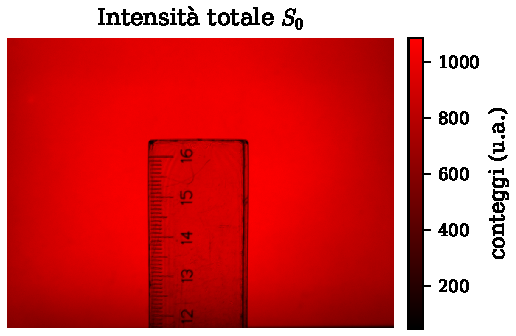
\includegraphics[height=0.205\textwidth]{Images/generated/righello_v2/R_S0.pdf}}\hfill
    \subfloat[$S_1$]{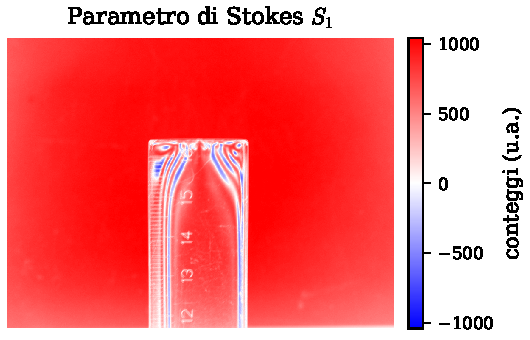
\includegraphics[height=0.205\textwidth]{Images/generated/righello_v2/R_S1.pdf}}\hfill
    \subfloat[$S_2$]{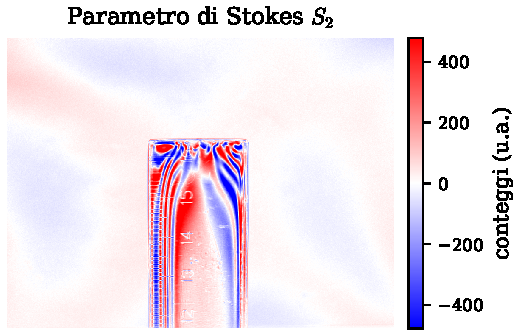
\includegraphics[height=0.205\textwidth]{Images/generated/righello_v2/R_S2.pdf}}\\
    \subfloat[$S_3$]{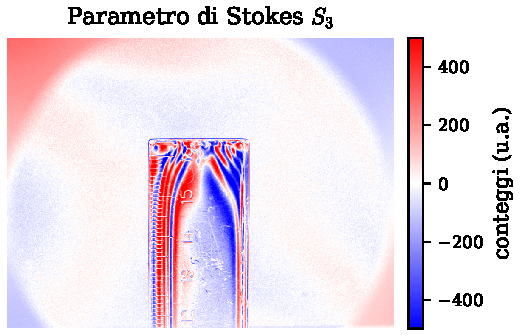
\includegraphics[height=0.205\textwidth]{Images/generated/righello_v2/R_S3.pdf}}\hfill
    \subfloat[DoLP]{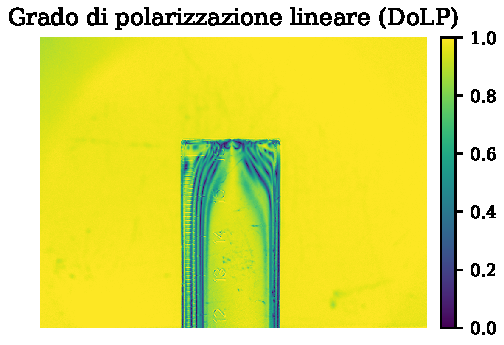
\includegraphics[height=0.205\textwidth]{Images/generated/righello_v2/R_DoLP.pdf}}\hfill
    \subfloat[AoLP]{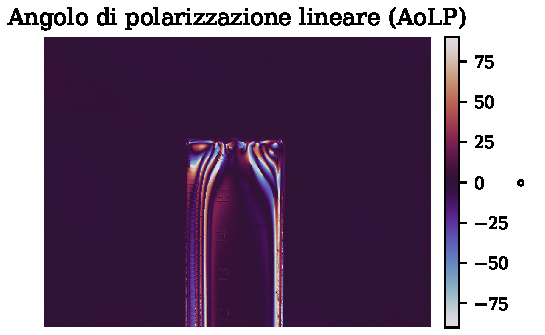
\includegraphics[height=0.205\textwidth]{Images/generated/righello_v2/R_AoLP.pdf}}
    \caption{Panoramica dei parametri polarimetrici per il righello in plastica trasparente, canale rosso. Le frange fotoelastiche dovute alle tensioni residue di stampaggio sono visibili nelle mappe di $S_1$, $S_2$ e in particolare del DoLP, dove le bande scure ($\mathrm{DoLP} \approx 0$) corrispondono ai punti in cui lo stato emergente è prossimo alla polarizzazione circolare (ritardanza pari a un multiplo dispari di $90^\circ$, con assi locali della birifrangenza a circa $45^\circ$ dalla polarizzazione incidente).}
    \label{fig:righello_overview}
\end{figure}

Le frange sono più leggibili nella mappa del DoLP: le bande scure, dove $\mathrm{DoLP} \approx 0$, segnano i luoghi in cui lo stato emergente è prossimo alla polarizzazione circolare, condizione che si realizza dove la ritardanza accumulata è un multiplo dispari di $90^\circ$ e gli assi locali della birifrangenza formano un angolo prossimo a $45^\circ$ con la polarizzazione incidente; dove la ritardanza è invece un multiplo intero di $\pi$ lo stato emergente torna linearmente polarizzato e il DoLP risale verso l'unità. La loro distribuzione spaziale ricalca l'andamento delle tensioni interne lungo il corpo del righello. Poiché la ritardanza dipende dalla lunghezza d'onda, lo stesso campo di sforzo produce frange più fitte alle lunghezze d'onda corte: la \cref{fig:righello_dolp_rgb} confronta la mappa del DoLP sui tre canali colore, e la frequenza spaziale delle frange cresce visibilmente dal rosso al blu, coerentemente con l'aumento della ritardanza al diminuire di $\lambda$.

\begin{figure}[H]
    \centering
    \subfloat[Canale R ($\lambda_\mathrm{eff} \approx \SI{626}{\nano\meter}$)]{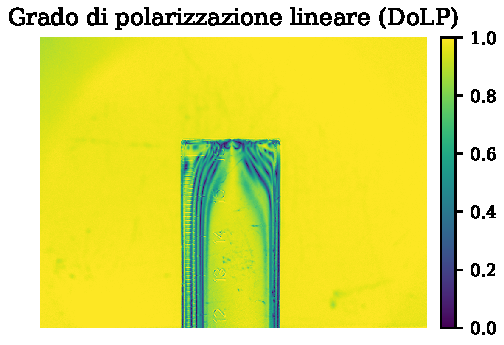
\includegraphics[height=0.205\textwidth]{Images/generated/righello_v2/R_DoLP.pdf}}\hfill
    \subfloat[Canale G ($\lambda_\mathrm{eff} \approx \SI{536}{\nano\meter}$)]{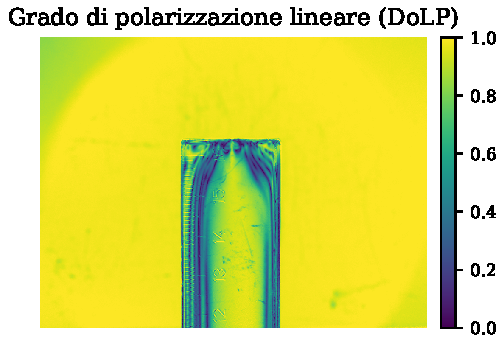
\includegraphics[height=0.205\textwidth]{Images/generated/righello_v2/G_DoLP.pdf}}\hfill
    \subfloat[Canale B ($\lambda_\mathrm{eff} \approx \SI{466}{\nano\meter}$)]{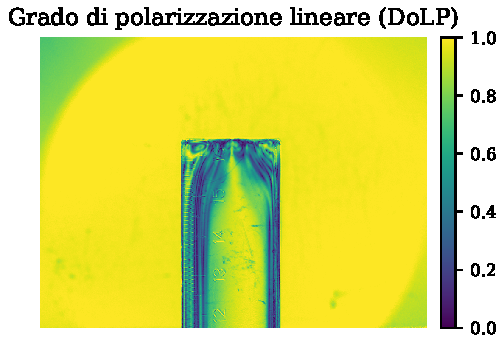
\includegraphics[height=0.205\textwidth]{Images/generated/righello_v2/B_DoLP.pdf}}
    \caption{Mappe del DoLP del righello sui tre canali del sensore. La frequenza spaziale delle frange fotoelastiche aumenta dal rosso al blu, manifestazione diretta della crescita della ritardanza al diminuire della lunghezza d'onda.}
    \label{fig:righello_dolp_rgb}
\end{figure}

L'esito è qualitativo ma significativo: senza alcuna calibrazione quantitativa il polarimetro restituisce mappe coerenti che rivelano la birifrangenza residua del materiale e la sua dipendenza spettrale, confermando il corretto funzionamento dell'intera catena di misura prima dei test di accuratezza presentati nelle sezioni successive.

% ---------------------------------------------------------------------------
\section{Calibrazione della correzione cromatica di \texorpdfstring{$S_3$}{S3}}
\label{sec:calibrazione_s3}

La ricostruzione di $S_3$ (\cref{eq:s3_formula}) contiene un unico parametro libero, il ritardo $\delta_a(\lambda)$ della lamina $\lambda/4$ impiegata come analizzatore, attraverso il fattore di correzione cromatica $1/\sin\delta_a(\lambda)$. Poiché ogni mappa di ritardanza e ogni mappa dell'asse veloce dei campioni birifrangenti dipendono da $S_3$, la scelta di $\delta_a(\lambda)$ condiziona l'intero capitolo. Adottarne un valore da un modello di materiale lascerebbe i risultati appesi a un'assunzione non verificata: il costruttore non dichiara né il materiale della lamina né il suo ordine. Si è perciò preferito \emph{misurare} $\delta_a(\lambda)$ direttamente dai dati, prima di applicare la pipeline ai campioni.

La misura sfrutta un'identità dell'apparato. La lamina $\lambda/4$ analizzata come campione nel dataset \texttt{lambdaquarti} è dello stesso tipo della lamina $\lambda/4$ inserita come analizzatore di $S_3$ in tutte le acquisizioni: le due condividono per costruzione lo stesso ritardo $\delta_a(\lambda)$. Misurare la ritardanza del campione equivale dunque a misurare la quantità che entra nella correzione. Il punto determinante è che questa misura può essere condotta senza ricorrere a $S_3$ e senza alcun modello di dispersione. I parametri lineari $S_0$, $S_1$, $S_2$ provengono dalle trentasei acquisizioni con il solo analizzatore lineare rotante, in cui la lamina $\lambda/4$ analizzatore non è presente nel cammino ottico; la ritardanza del campione vi è impressa attraverso la conversione dello stato di polarizzazione incidente, e il suo modulo è fissato dal canale coseno, costruito sui soli $S_0$, $S_1$, $S_2$. Il segno di $\delta_a$, e con esso il completamento a $[0^\circ, 360^\circ)$, non serve alla correzione, che dipende dal solo $\sin\delta_a$.

Resta da rendere la stima immune da due effetti che, se trascurati, la distorcerebbero. Il primo è la depolarizzazione introdotta dalla lamina, che riduce il grado di polarizzazione totale dal valore prossimo all'unità dello sfondo a circa $0{,}9$ nel rosso e $0{,}8$ nel blu: normalizzare sul livello dello sfondo, come fa il canale coseno, spinge artificiosamente la ritardanza verso $90^\circ$. Il secondo è l'ellitticità residua del fascio incidente, già rimossa nella pipeline dalla rotazione di Poincaré attorno all'asse $S_2$ (\cref{sec:ellitticita}). Entrambi si neutralizzano lavorando con i \emph{rapporti} fra le componenti del vettore di Stokes, ovvero con la sua direzione: sotto depolarizzazione scalare il fattore di depolarizzazione $p$ moltiplica tutte le componenti e si elide nei rapporti, lasciando inalterata la direzione dell'ellisse e quindi la ritardanza. La direzione del vettore, ricostruita sui pixel della lamina dopo gli allineamenti, fornisce così una stima di $\delta_a$ indipendente dalla normalizzazione di sfondo.

L'ultimo ingrediente chiude il problema senza introdurre circolarità. La differenza grezza $I_{-45} - I_{+45}$, non ancora divisa per $\sin\delta_a$, raccoglie due fattori $\sin\delta_a$: uno introdotto dalla lamina-campione nel convertire la polarizzazione, l'altro dall'analizzatore identico nel rivelarla. Vale pertanto, per uno stato incidente lineare di riferimento,
\begin{equation}
    I_{-45} - I_{+45} \;\propto\; p \, \sin 2\theta \, \sin^2\!\delta_a,
    \label{eq:s3_selfref}
\end{equation}
dove $\theta$ è l'orientazione dell'asse della lamina. Il ritardo $\delta_a$ vi compare al quadrato e si auto-riferisce: rapportando la \cref{eq:s3_selfref} alle componenti lineari $S_1$, $S_2$, nelle quali $p$ si elide, si ottiene un sistema di due equazioni nelle due incognite $\delta_a$ e $\theta$, risolto in modo auto-consistente con la rotazione di Poincaré effettivamente usata nella pipeline. La soluzione non assume alcun materiale, alcun ordine, né la correzione che si intende calibrare.

I valori così ottenuti sono riportati nella \cref{tab:s3_calibrazione}. La bontà interna della procedura è confermata da due verifiche che non sono state imposte ma emergono dalla soluzione: il fattore di depolarizzazione $p$ ricostruito dall'inversione riproduce il grado di polarizzazione totale misurato indipendentemente sui tre canali, decrescente verso il blu, e l'orientazione $\theta$ risulta uniforme fra i canali, come deve essere per una lamina spazialmente omogenea osservata a un'unica orientazione meccanica. La sola legge geometrica di un ritardatore a singolo ordine (\cref{eq:dispersione-qwp} a dispersione trascurata), ancorata al punto di design e indipendente dal materiale, fornisce $91{,}0^\circ$, $106{,}3^\circ$ e $122{,}3^\circ$ sui tre canali: la ritardanza misurata la segue al canale rosso e se ne discosta in eccesso crescente verso il blu ($+4{,}7^\circ$ al verde, $+8{,}5^\circ$ al blu), come mostra la \cref{fig:s3_calibration}. È l'andamento atteso in presenza di dispersione normale della birifrangenza, il cui contributo si somma al fattore geometrico $1/\lambda$; la compatibilità della lamina con un singolo ordine ne risulta confermata a posteriori, mentre il materiale resta fuori dalla catena di misura: a tre bande spettrali larghe i modelli di dispersione dei polimeri comuni da film ritardatori e dei cristalli birifrangenti riproducono i tre punti in modo pressoché equivalente, e non è identificabile.

\begin{table}[H]
    \centering
    \caption{Ritardanza $\delta_a$ della lamina $\lambda/4$ analizzatore, misurata direttamente dal dataset \texttt{lambdaquarti} in modo non circolare, depol-unbiased e indipendente dal materiale (vedi testo), e fattore di correzione cromatica $1/\sin\delta_a$ adottato nella ricostruzione di $S_3$. L'ultima colonna riporta, come riferimento indipendente dal materiale, la sola legge geometrica $\delta_0\,\lambda_0/\lambda$ di un ritardatore a singolo ordine ancorata al punto di design, che non interviene nella misura: l'eccesso della misura, crescente verso il blu, riflette la dispersione normale della birifrangenza del materiale, non identificabile a tre bande larghe. Al canale rosso $\delta_a \approx 90^\circ$ rende la correzione prossima all'unità e quindi insensibile a ogni scelta di modello.}
    \label{tab:s3_calibrazione}
    \begin{tabular}{lcccc}
        \hline
        \textbf{Canale} & $\lambda_\mathrm{eff}$ [\si{\nano\meter}] & $\delta_a$ misurato [\si{\degree}] & $1/\sin\delta_a$ & $\delta_a$ geom.\ $1/\lambda$ [\si{\degree}] \\
        \hline
        Rosso & 626 & $88{,}4$  & $1{,}000$ & $91{,}0$  \\
        Verde & 536 & $111{,}0$ & $1{,}071$ & $106{,}3$ \\
        Blu   & 466 & $130{,}8$ & $1{,}321$ & $122{,}3$ \\
        \hline
    \end{tabular}
\end{table}

\begin{figure}[H]
    \centering
    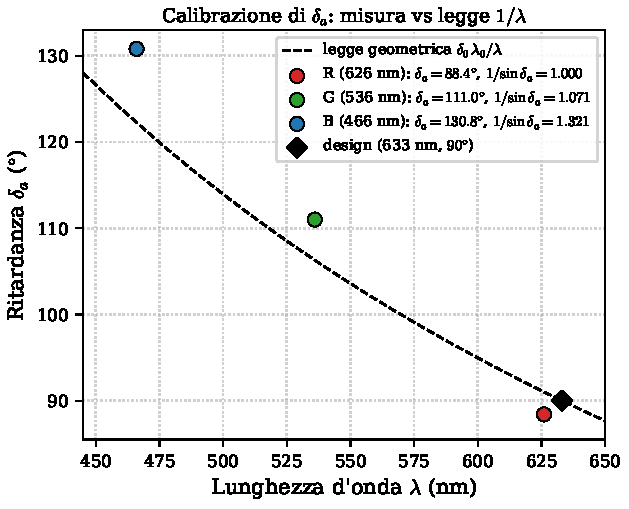
\includegraphics[width=0.62\textwidth]{Images/generated/lambdaquarti_50deg/s3_calibration.pdf}
    \caption{Calibrazione della ritardanza $\delta_a$ dell'analizzatore $\lambda/4$. I tre punti colorati sono i valori misurati direttamente dal dataset \texttt{lambdaquarti} in modo non circolare e indipendente dal materiale; la curva tratteggiata è la sola legge geometrica $\delta_0\,\lambda_0/\lambda$ di un ritardatore a singolo ordine, ancorata al punto di design (diamante nero, $\lambda_0 = \SI{633}{\nano\meter}$, $\delta_0 = 90^\circ$): \emph{non} un fit ai punti ma il riferimento minimo indipendente dal materiale. La misura la segue al rosso e cresce più ripidamente verso il blu, come atteso in presenza di dispersione normale della birifrangenza; la correzione $1/\sin\delta_a$ riportata in legenda cresce dal rosso, dove è prossima all'unità, al blu.}
    \label{fig:s3_calibration}
\end{figure}

L'adozione di questa correzione misurata, in luogo di quella calcolata da un tipico modello di dispersione di lamina a singolo ordine, sposta la ritardanza ricostruita dei campioni di non più di circa un grado, blu compreso, e lascia invariate le pendenze del nastro stratificato analizzato nella \cref{sec:risultati_nastro}. Questa insensibilità è essa stessa un risultato: la ricostruzione della ritardanza non dipende in modo critico dal modello di dispersione adottato per $S_3$, e l'obiezione di principio sulla scelta del materiale della lamina perde mordente sul piano quantitativo. Le sezioni seguenti applicano la correzione calibrata a campioni di ritardanza nota e crescente.

% ---------------------------------------------------------------------------
\section{Accuratezza della ricostruzione: lamine d'onda}
\label{sec:risultati_lamine}

\subsection{Lamina \texorpdfstring{$\lambda/4$}{lambda/4}}
\label{subsec:risultati_qw}

La lamina quarto d'onda ($\lambda_0 = \SI{633}{\nano\meter}$), orientata a circa \SI{50}{\degree}, è stata analizzata sui tre canali colore con la procedura comune a entrambe le lamine d'onda. Questo campione ha un ruolo speciale: è dello stesso tipo della lamina $\lambda/4$ impiegata come analizzatore di $S_3$, ed è dal suo dataset che si ricava la calibrazione non circolare della correzione cromatica di $S_3$ (\cref{sec:calibrazione_s3}). Analizzata qui come campione attraverso la pipeline completa, con la correzione già calibrata, ne riproduce per costruzione la ritardanza e ne documenta l'uniformità spaziale; il controllo di accuratezza genuino, il confronto fra ritardanza misurata e legge geometrica di singolo ordine senza assunzioni sul materiale, è quello discusso nella sezione di calibrazione.

La struttura del campione è visibile nelle mappe di intensità $S_0$ in \cref{fig:qw_s0}: il disco centrale corrisponde alla lamina a ritardanza uniforme, l'anello scuro alla montatura circolare che la sostiene, e lo sfondo libero alla luce diretta del display LCD, dove la ritardanza è prossima a zero.

\begin{figure}[H]
    \centering
    \subfloat[Canale R ($\lambda_\mathrm{eff} \approx \SI{626}{\nano\meter}$)]{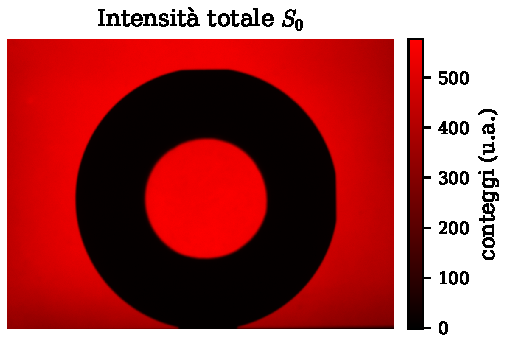
\includegraphics[height=0.205\textwidth]{Images/generated/lambdaquarti_50deg/R_S0.pdf}}\hfill
    \subfloat[Canale G ($\lambda_\mathrm{eff} \approx \SI{536}{\nano\meter}$)]{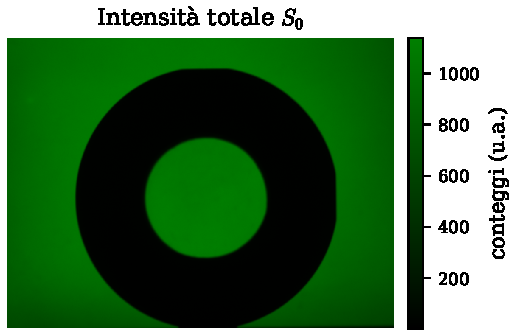
\includegraphics[height=0.205\textwidth]{Images/generated/lambdaquarti_50deg/G_S0.pdf}}\hfill
    \subfloat[Canale B ($\lambda_\mathrm{eff} \approx \SI{466}{\nano\meter}$)]{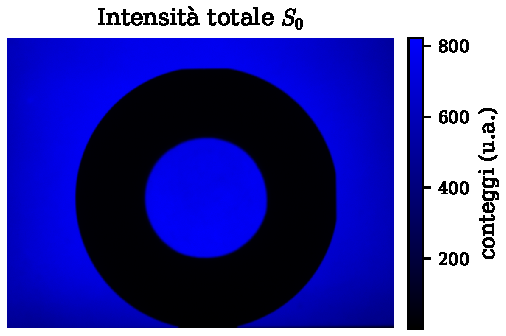
\includegraphics[height=0.205\textwidth]{Images/generated/lambdaquarti_50deg/B_S0.pdf}}
    \caption{Mappe di intensità $S_0$ per la lamina $\lambda/4$ sui tre canali del sensore. Il disco centrale corrisponde alla lamina, l'anello scuro alla montatura, lo sfondo all'illuminazione diretta del display LCD.}
    \label{fig:qw_s0}
\end{figure}

Le mappe dell'orientazione dell'asse veloce $\theta$ e della ritardanza $\delta$ sono riportate per i tre canali in \cref{fig:qw_theta_delta}. L'asse veloce è uniforme entro il disco della lamina, su un valore prossimo a $34^\circ$; lo scarto rispetto all'orientazione meccanica nominale di \SI{50}{\degree} corrisponde all'offset fra il riferimento del supporto della lamina e l'asse di polarizzazione incidente del display, rispetto al quale la pipeline misura tutti gli angoli polarimetrici (\cref{sec:allineamento}). La ritardanza è uniforme nello stesso disco e cresce dal canale rosso al canale blu, secondo la dispersione $\delta \propto 1/\lambda$ attesa per una lamina a singolo ordine. Le code di rumore aumentano verso il blu, dove il rapporto segnale-rumore di $S_3$ peggiora a causa della maggiore correzione cromatica applicata.

\begin{figure}[H]
    \centering
    \subfloat[$\theta$ , canale R]{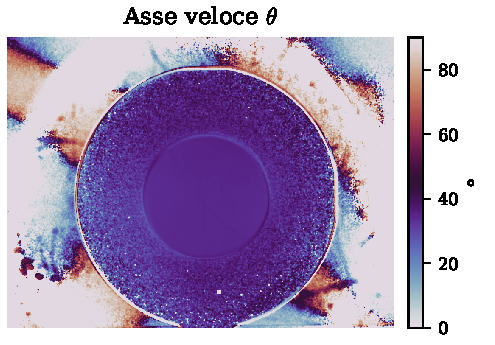
\includegraphics[height=0.205\textwidth]{Images/generated/lambdaquarti_50deg/R_theta.pdf}}\hfill
    \subfloat[$\theta$ , canale G]{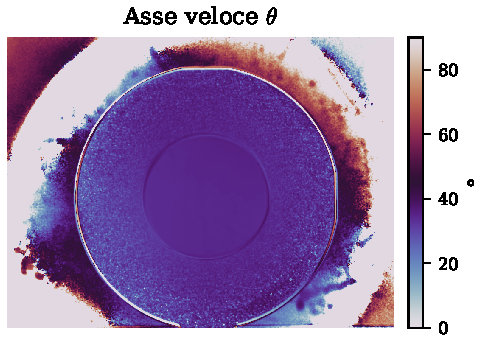
\includegraphics[height=0.205\textwidth]{Images/generated/lambdaquarti_50deg/G_theta.pdf}}\hfill
    \subfloat[$\theta$ , canale B]{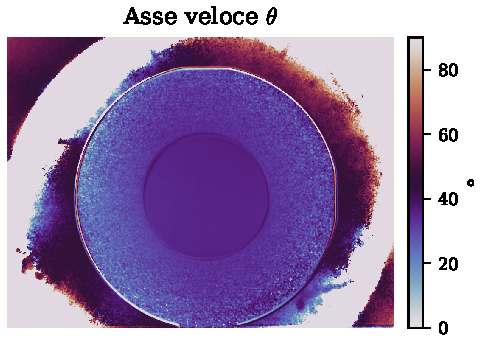
\includegraphics[height=0.205\textwidth]{Images/generated/lambdaquarti_50deg/B_theta.pdf}}\\
    \subfloat[$\delta$ , canale R]{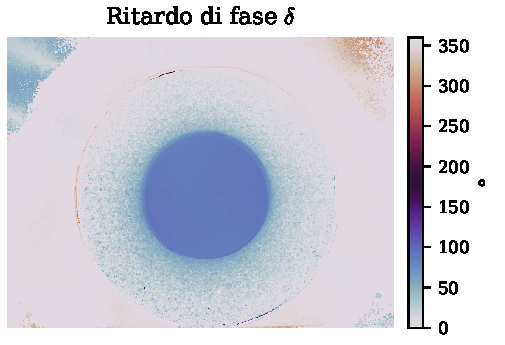
\includegraphics[height=0.205\textwidth]{Images/generated/lambdaquarti_50deg/R_delta.pdf}}\hfill
    \subfloat[$\delta$ , canale G]{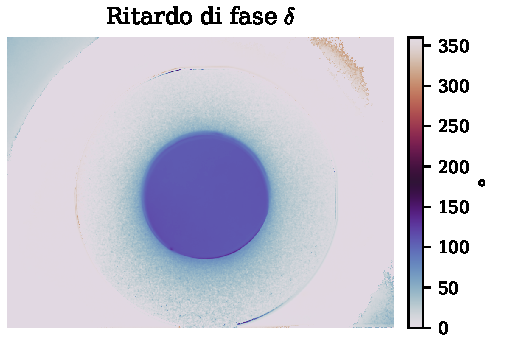
\includegraphics[height=0.205\textwidth]{Images/generated/lambdaquarti_50deg/G_delta.pdf}}\hfill
    \subfloat[$\delta$ , canale B]{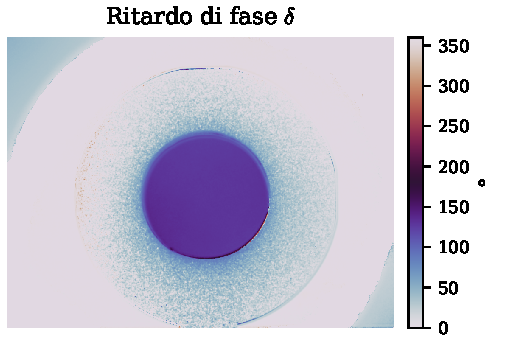
\includegraphics[height=0.205\textwidth]{Images/generated/lambdaquarti_50deg/B_delta.pdf}}
    \caption{Mappe dell'orientazione dell'asse veloce $\theta$ (riga superiore) e della ritardanza $\delta$ (riga inferiore) per la lamina $\lambda/4$, sui tre canali del sensore. L'asse veloce è uniforme entro il disco della lamina; la ritardanza cresce dal rosso al blu secondo la dispersione $\delta \propto 1/\lambda$ di una lamina a singolo ordine.}
    \label{fig:qw_theta_delta}
\end{figure}

La conversione della polarizzazione lineare in circolare, funzione caratteristica di una lamina quarto d'onda, è verificata direttamente dal modulo della componente circolare normalizzata nel disco. Per una lamina con asse veloce a $\theta$ e ritardanza $\delta_a$ il modello di propagazione (\cref{eq:s3_ritardatore}) prevede $|s_3| = \sin 2\theta \, \sin\delta_a \, p$, dove $p$ è il grado di polarizzazione locale: con $\theta \approx 34^\circ$ e i valori calibrati di $\delta_a$, l'atteso è $0{,}84$, $0{,}72$ e $0{,}57$ sui tre canali, contro valori misurati di $0{,}82$, $0{,}69$ e $0{,}54$, in accordo entro $0{,}03$. Il valore unitario del caso ideale, lamina a $45^\circ$ e luce completamente polarizzata, non viene raggiunto perché l'orientazione effettiva rispetto alla polarizzazione incidente è di circa $34^\circ$ e la lamina depolarizza parzialmente il fascio.

La stima quantitativa della ritardanza segue la stessa pipeline di clustering della \cref{sec:umap_clustering}: il cluster vincente HDBSCAN sull'embedding UMAP individua i pixel del disco della lamina e ne fornisce la mediana $\tilde\delta_{\mathrm{win}}$. Le tre stime per-canale, ottenute processando la lamina come campione con la correzione di $S_3$ calibrata, sono raccolte nella \cref{tab:qw_ritardanza} e confrontate con la legge geometrica di singolo ordine ancorata al design. La dispersione interna del cluster vincente, quantificata dalla deviazione mediana assoluta circolare, non supera $1{,}2^\circ$ su alcun canale: si tratta di un indicatore dell'omogeneità della regione selezionata, da non confondersi con l'accuratezza assoluta della misura (\cref{sec:discussione}). Esse coincidono per costruzione con la calibrazione (\cref{tab:s3_calibrazione}) a meno di una lieve differenza, più marcata al blu, dovuta al bias di depolarizzazione della lettura combinata coseno-seno della ritardanza, che tende a riavvicinare il valore a $90^\circ$. Le stime sono fittate con la legge di dispersione $\delta(\lambda) = k/\lambda$ di una lamina a singolo ordine; il punto di design $(\lambda_0 = \SI{633}{\nano\meter},\,\delta_0 = 90^\circ)$ è riportato come riferimento ma non incluso nel fit, condotto sui soli tre punti misurati. Il risultato è in \cref{fig:qw_delta_fit}.

\begin{table}[H]
    \centering
    \caption{Ritardanza della lamina $\lambda/4$ analizzata \emph{come campione} ($\lambda_0 = \SI{633}{\nano\meter}$), estratta dalla mediana del cluster vincente HDBSCAN sull'embedding UMAP e processata con la correzione di $S_3$ calibrata (\cref{sec:calibrazione_s3}), confrontata con la sola legge geometrica $\delta(\lambda) = 90^\circ \cdot \lambda_0/\lambda$ di un ritardatore a singolo ordine, indipendente dal materiale. Lo scarto, in eccesso crescente verso il blu, ingloba il contributo fisico della dispersione normale della birifrangenza, che si somma al fattore $1/\lambda$. La lieve differenza rispetto ai valori di calibrazione (\cref{tab:s3_calibrazione}), più marcata al blu, riflette il bias di depolarizzazione della lettura combinata coseno-seno della ritardanza.}
    \label{tab:qw_ritardanza}
    \begin{tabular}{lcccc}
        \hline
        \textbf{Canale} & $\lambda_\mathrm{eff}$ [\si{\nano\meter}] & $\tilde\delta_\mathrm{win}$ [\si{\degree}] & $\delta_\mathrm{geom}$ [\si{\degree}] & Scarto [\si{\degree}] \\
        \hline
        Rosso & 626 & $87{,}1$  & $91{,}0$  & $-3{,}9$ \\
        Verde & 536 & $108{,}6$ & $106{,}3$ & $+2{,}3$ \\
        Blu   & 466 & $128{,}5$ & $122{,}3$ & $+6{,}2$ \\
        \hline
    \end{tabular}
\end{table}

\begin{figure}[H]
    \centering
    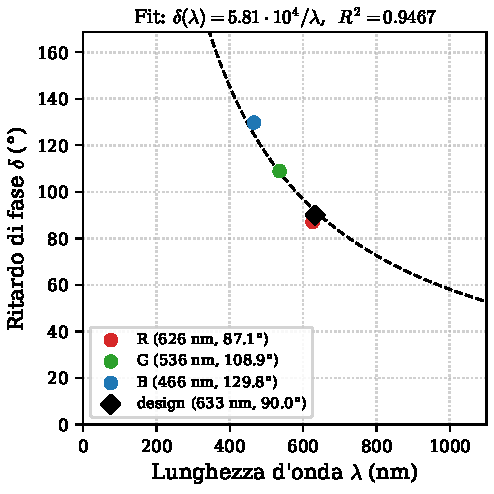
\includegraphics[width=0.55\textwidth]{Images/generated/lambdaquarti_50deg/delta_lambda_fit.pdf}
    \caption{Fit di dispersione $\delta(\lambda) = k/\lambda$ sulla lamina $\lambda/4$. I tre punti colorati sono le stime $\tilde\delta_{\mathrm{win}}$ del cluster vincente HDBSCAN per ciascun canale; il diamante nero è il punto di design $(\lambda_0 = \SI{633}{\nano\meter},\,\delta_0 = 90^\circ)$, riportato come riferimento e non incluso nel fit. La curva tratteggiata è il fit non lineare ai minimi quadrati sui soli tre punti misurati.}
    \label{fig:qw_delta_fit}
\end{figure}

\subsection{Lamina \texorpdfstring{$\lambda/2$}{lambda/2}}
\label{subsec:risultati_hw}

La lamina mezz'onda, di cui il costruttore dichiara la sola ritardanza nominale di mezz'onda alla lunghezza d'onda di design $\lambda_0 = \SI{633}{\nano\meter}$, orientata a circa \SI{50}{\degree}, è stata analizzata sui tre canali colore con l'obiettivo di validare la ricostruzione della ritardanza in un regime di forte dispersione cromatica, oltre la lunghezza d'onda di progetto; come si vedrà, la misura rivela un ritardatore con dispersione di ritardanza \emph{inversa}, della famiglia dei ritardatori a largo spettro, informazione non deducibile dall'etichetta. La struttura macroscopica del campione è visibile nelle mappe di intensità $S_0$ in \cref{fig:hw_s0}: si distingue il disco centrale della lamina, la montatura metallica circolare che la sostiene e lo sfondo libero illuminato dal display LCD. Il contrasto fra le tre acquisizioni RGB riflette unicamente la trasmissività spettrale del sistema sorgente-lamina-sensore e non dipende dallo stato di polarizzazione locale.

\begin{figure}[H]
    \centering
    \subfloat[Canale R ($\lambda_\mathrm{eff} \approx \SI{626}{\nano\meter}$)]{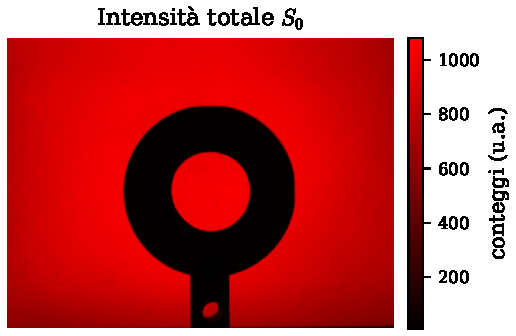
\includegraphics[height=0.205\textwidth]{Images/generated/lambdamezzi_50deg/R_S0.pdf}}\hfill
    \subfloat[Canale G ($\lambda_\mathrm{eff} \approx \SI{536}{\nano\meter}$)]{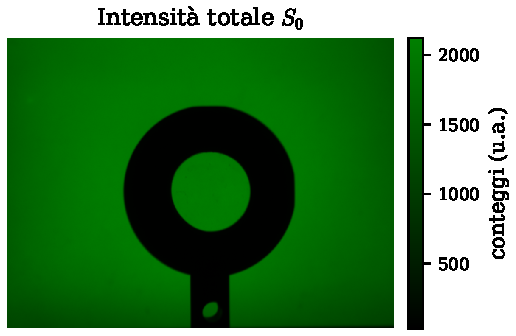
\includegraphics[height=0.205\textwidth]{Images/generated/lambdamezzi_50deg/G_S0.pdf}}\hfill
    \subfloat[Canale B ($\lambda_\mathrm{eff} \approx \SI{466}{\nano\meter}$)]{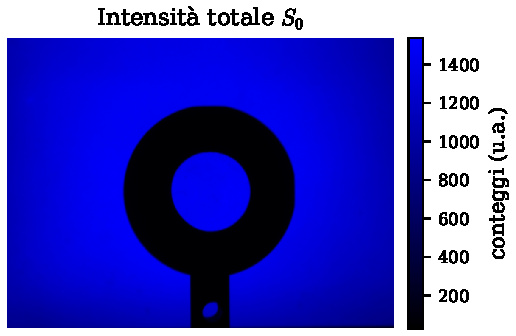
\includegraphics[height=0.205\textwidth]{Images/generated/lambdamezzi_50deg/B_S0.pdf}}
    \caption{Mappe di intensità $S_0$ per la lamina $\lambda/2$ sui tre canali del sensore. Il disco centrale corrisponde alla lamina, l'anello scuro alla montatura, lo sfondo all'illuminazione diretta del display LCD.}
    \label{fig:hw_s0}
\end{figure}

Le mappe dell'orientazione dell'asse veloce $\theta$ e della ritardanza $\delta$ sono riportate per i tre canali colore in \cref{fig:hw_theta_delta}. L'asse veloce risulta uniforme entro il disco della lamina, su un valore prossimo a $38^\circ$; lo scarto rispetto all'orientazione meccanica nominale di \SI{50}{\degree} corrisponde all'offset fra il riferimento del supporto della lamina e l'asse di polarizzazione incidente del display, rispetto al quale la pipeline misura tutti gli angoli polarimetrici (\cref{sec:allineamento}), e la differenza di qualche grado rispetto all'offset della lamina $\lambda/4$ (asse a circa $34^\circ$, \cref{subsec:risultati_qw}) rientra nella tolleranza dell'impostazione manuale dell'orientazione sul supporto. La ritardanza è anch'essa uniforme nel disco, ma il suo valore \emph{decresce} passando dal canale rosso al canale blu, in direzione opposta a quella attesa per una lamina a singolo ordine, in cui $\delta \propto 1/\lambda$ cresce verso le lunghezze d'onda corte. L'algoritmo di estrazione discusso nella \cref{subsec:modello_retardance} restituisce $\delta$ nell'intervallo $[0^\circ, 360^\circ)$ tramite $\arctan_2(\sin\delta, \cos\delta)$, con il segno di $\sin\delta$ fissato univocamente dal parametro $S_3$; il valore ricostruito è pertanto privo di ambiguità e questa decrescita è una caratteristica genuina del dato, la cui interpretazione è sviluppata più avanti.

\begin{figure}[H]
    \centering
    \subfloat[$\theta$ , canale R]{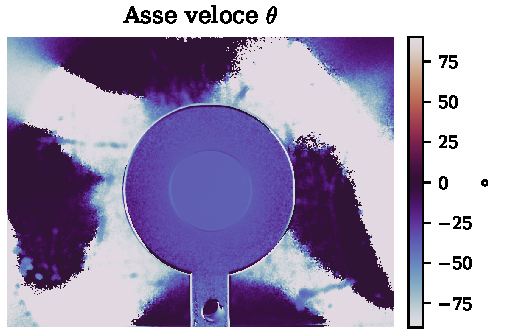
\includegraphics[height=0.205\textwidth]{Images/generated/lambdamezzi_50deg/R_theta.pdf}}\hfill
    \subfloat[$\theta$ , canale G]{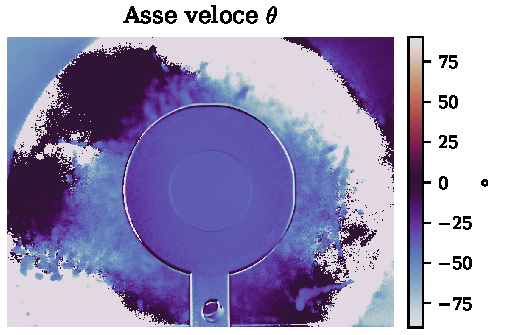
\includegraphics[height=0.205\textwidth]{Images/generated/lambdamezzi_50deg/G_theta.pdf}}\hfill
    \subfloat[$\theta$ , canale B]{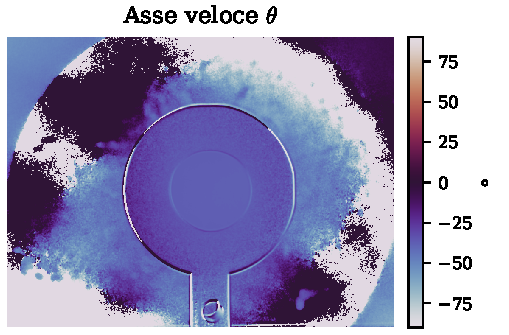
\includegraphics[height=0.205\textwidth]{Images/generated/lambdamezzi_50deg/B_theta.pdf}}\\
    \subfloat[$\delta$ , canale R]{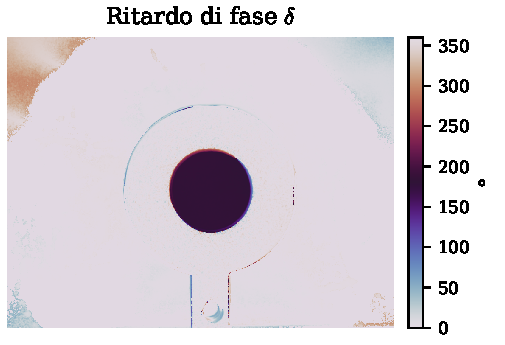
\includegraphics[height=0.205\textwidth]{Images/generated/lambdamezzi_50deg/R_delta.pdf}}\hfill
    \subfloat[$\delta$ , canale G]{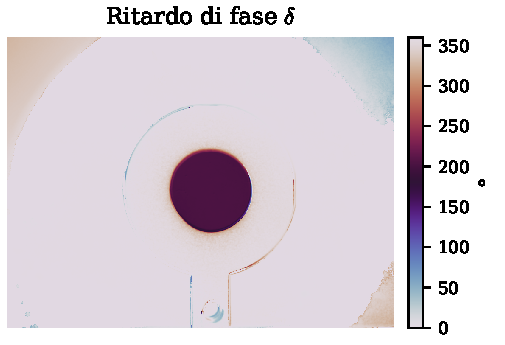
\includegraphics[height=0.205\textwidth]{Images/generated/lambdamezzi_50deg/G_delta.pdf}}\hfill
    \subfloat[$\delta$ , canale B]{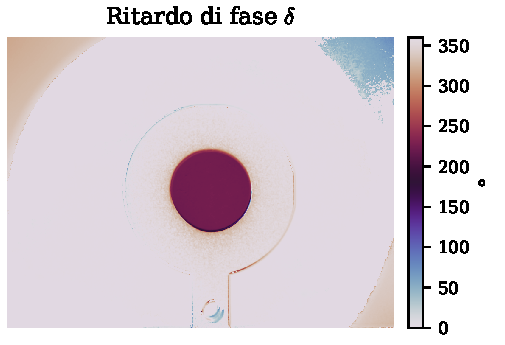
\includegraphics[height=0.205\textwidth]{Images/generated/lambdamezzi_50deg/B_delta.pdf}}
    \caption{Mappe dell'orientazione dell'asse veloce $\theta$ (riga superiore) e della ritardanza $\delta$ (riga inferiore) per la lamina $\lambda/2$, sui tre canali del sensore. L'asse veloce è uniforme entro il disco della lamina; la ritardanza, anch'essa uniforme, \emph{decresce} dal rosso al blu, in direzione opposta alla legge $\delta \propto 1/\lambda$ di un ritardatore a dispersione normale. Tale comportamento, dopo l'esclusione quantitativa delle spiegazioni alternative, è attribuito nel testo a una dispersione di ritardanza inversa (ritardatore a largo spettro). La \emph{colormap} ciclica \texttt{twilight} sull'intero giro $[0^\circ, 360^\circ)$ è impiegata per $\delta$.}
    \label{fig:hw_theta_delta}
\end{figure}

La funzione caratteristica di una lamina mezz'onda, la rotazione dell'azimut di polarizzazione di un angolo pari al doppio dell'orientazione dell'asse, è verificata sull'AoLP del disco. Al canale rosso, dove la ritardanza misurata di $\approx 177^\circ$ è prossima alla mezz'onda ideale, l'AoLP del cluster della lamina vale $+75{,}7^\circ$, in accordo entro un grado con il valore $2\theta \approx 76^\circ$ atteso per l'asse a $\theta \approx 38^\circ$; sui canali verde e blu l'AoLP scende progressivamente a $+72{,}8^\circ$ e $+70{,}4^\circ$, coerentemente con l'allontanamento della ritardanza dal valore di mezz'onda, che rende lo stato uscente ellittico e ne sposta l'azimut.

Per ottenere una stima quantitativa della ritardanza non condizionata da scelte soggettive della regione di interesse si è ricorsi alla pipeline di clustering descritta nella \cref{sec:umap_clustering}: il vettore di feature $(s_1, s_2, s_3, \mathrm{DoLP})$ viene proiettato in due dimensioni tramite UMAP e l'embedding viene segmentato con HDBSCAN. Il cluster di sfondo, che concentra la maggior parte della massa statistica, identifica la posizione angolare di riferimento sul cerchio di $\delta$; il cluster vincente, individuato dallo score $\mathcal{S}_k = f_k \cdot R_k \cdot (\Delta\delta_k)^2$, coincide con i pixel della lamina e fornisce direttamente la stima $\tilde\delta_{\mathrm{win}}$. La quadratura della distanza angolare penalizza i grandi cluster centrati sulla mediana globale, sterilizzando il rischio di selezionare lo sfondo come falso positivo. Le tre stime $\tilde\delta_R$, $\tilde\delta_G$, $\tilde\delta_B$ così ottenute alle rispettive lunghezze d'onda centroidi, con una deviazione mediana assoluta entro il cluster inferiore a $0{,}6^\circ$ su tutti i canali, sono raccolte nella \cref{tab:hw_ritardanza} e confrontate con la previsione $\delta(\lambda) = k/\lambda$ propria di una lamina a singolo ordine (\cref{eq:fit_dispersione} con $p=1$), normalizzata al punto di design $(\lambda_0 = \SI{633}{\nano\meter},\,\delta_0 = 180^\circ)$ dichiarato dal costruttore.

\begin{table}[H]
    \centering
    \caption{Ritardanza della lamina $\lambda/2$ estratta dalla mediana del cluster vincente HDBSCAN sull'embedding UMAP, confrontata con la previsione a singolo ordine $\delta_\mathrm{teorico} = \delta_0 \cdot \lambda_0/\lambda$ ($\delta_0 = 180^\circ$ alla lunghezza d'onda di design $\lambda_0 = \SI{633}{\nano\meter}$). Questa è la dipendenza minima attesa per un ritardatore a singolo passaggio in regime di dispersione normale, fissata dal solo fattore geometrico $1/\lambda$; la dispersione di birifrangenza, se normale, non farebbe che accentuarne la crescita verso il blu. La ritardanza misurata \emph{decresce} invece verso il blu, in direzione opposta alla previsione, che \emph{cresce}: la lamina non è riconducibile a un ritardatore a dispersione normale, e l'analisi nel testo esclude quantitativamente anche l'avvolgimento multi-ordine, attribuendo la decrescita a una dispersione di ritardanza inversa.}
    \label{tab:hw_ritardanza}
    \begin{tabular}{lcccc}
        \hline
        \textbf{Canale} & $\lambda_\mathrm{eff}$ [\si{\nano\meter}] & $\tilde\delta_\mathrm{win}$ [\si{\degree}] & $\delta_\mathrm{teorico}$ [\si{\degree}] & Scarto [\si{\degree}] \\
        \hline
        Rosso & 626 & $176{,}9$ & $182{,}0$ & $-5{,}1$ \\
        Verde & 536 & $156{,}8$ & $212{,}6$ & $-55{,}8$ \\
        Blu   & 466 & $134{,}5$ & $244{,}5$ & $-110{,}0$ \\
        \hline
    \end{tabular}
\end{table}

I tre valori misurati decrescono in modo monotono dal rosso al blu ($176{,}9 \to 156{,}8 \to 134{,}5^\circ$), in direzione opposta alla previsione a dispersione normale, che cresce ($182{,}0 \to 212{,}6 \to 244{,}5^\circ$). Per un ritardatore attraversato una sola volta vale $\delta = 2\pi\,\Delta n(\lambda)\,d/\lambda$, e in regime di dispersione normale entrambi i fattori spingono $\delta$ verso l'alto alle lunghezze d'onda corte. Conviene riformulare il dato in termini di ritardo ottico $\mathrm{Re} = \delta\,\lambda/360^\circ = \Delta n\, d$, la grandezza propria del materiale, depurata dal fattore geometrico: la misura corrisponde a $\mathrm{Re} = 308 \to 233 \to 174$~nm dal rosso al blu. Su una lamina priva di marcature, peraltro, l'assegnazione di quale asse sia il veloce è intrinsecamente ambigua, e l'assegnazione complementare ($\delta \to 360^\circ - \delta$, ovvero $183{,}1/203{,}2/225{,}5^\circ$) fornisce $\mathrm{Re} = 318 \to 303 \to 292$~nm: il ritardo ottico decresce verso il blu in entrambi i casi, del $43\%$ o dell'$8\%$ rispettivamente, sicché la conclusione qualitativa non dipende dall'ambiguità. Un fit empirico $\delta = k/\lambda^{\,n}$ restituisce $n \approx -0{,}9$ sul ramo misurato e $n \approx +0{,}7$ sul complementare: in entrambi i casi $|n| < 1$, mentre la dispersione normale impone $n \geq 1$.

Prima di interpretare il dato si sono vagliate le spiegazioni più economiche. Un errore sistematico della catena di analisi è escluso dal riscontro della lamina $\lambda/4$ (\cref{sec:calibrazione_s3}), che con lo stesso modello di Stokes, la stessa correzione cromatica di $S_3$ e le stesse lunghezze d'onda effettive cresce verso il blu come atteso. Un'inversione prodotta da assi veloce e lento scambiati è già contenuta nell'ambiguità di assegnazione discussa sopra e non cambia il verso del ritardo ottico; il modulo della componente circolare normalizzata fornisce in ogni caso un controllo indipendente da qualunque convenzione di segno: $|s_3|$ misurato nel disco vale $0{,}05/0{,}31/0{,}53$ sui tre canali, in accordo entro $0{,}02$ con il modello $p \sin 2\theta\, |\sin\delta|$ valutato sui valori misurati, mentre la dispersione normale ($\delta = 213/246^\circ$ a G/B) predirebbe $0{,}44/0{,}70$, incompatibile. Una depolarizzazione differenziale del campione è infine esclusa dal grado di polarizzazione, identico fra le due lamine a ciascun canale.

L'ipotesi a prima vista più naturale resta allora l'avvolgimento: una lamina \emph{multi-ordine}, la cui ritardanza vera supera più giri di $360^\circ$, campionata su tre sole bande spettrali, può mostrare valori avvolti che procedono all'indietro per sotto-campionamento, in analogia con l'effetto stroboscopico per cui una ruota in rapida rotazione appare girare al contrario in una ripresa a basso numero di fotogrammi. Questa interpretazione, in apparenza la più semplice, è però falsificabile con i dati a disposizione, perché i canali del sensore non sono monocromatici. Su una banda di larghezza finita la ritardanza vera di un multi-ordine varia di molte decine o centinaia di gradi, e la sovrapposizione incoerente degli stati uscenti depolarizza il segnale: la frazione di polarizzazione conservata dalla media di banda è
\begin{equation}
    |V| = \frac{\left|\int I(\lambda)\, e^{i\,\delta(\lambda)}\, d\lambda\right|}{\int I(\lambda)\, d\lambda},
    \label{eq:band_retention}
\end{equation}
dove $I(\lambda)$ è lo spettro efficace del canale. Valutata sugli spettri efficaci misurati (banda verde di larghezza $\approx \SI{40}{\nano\meter}$), la \cref{eq:band_retention} prevede per il canale verde $|V| \leq 0{,}74$ già all'ordine $2$ e $|V| \leq 0{,}4$ all'ordine $5$, cui corrisponde un grado di polarizzazione complessivo inferiore a $0{,}78$ e $0{,}5$ rispettivamente. Il valore misurato all'interno del disco è $0{,}85$, indistinguibile da quello della lamina $\lambda/4$ ($0{,}83$), che opera a ordine zero: l'avvolgimento multi-ordine è escluso, per qualunque scelta ragionevole del modello di banda. Lo stesso argomento, applicato alla $\lambda/4$, ne conferma a posteriori l'ordine zero.

Escluse le alternative, la decrescita è una proprietà reale del componente: la lamina è un ritardatore a basso ordine la cui dispersione di ritardanza è \emph{inversa}, con $\mathrm{Re}$ decrescente verso le lunghezze d'onda corte. Per un materiale naturale in regime di trasparenza questo comportamento sarebbe sorprendente, ed è per questo che l'ipotesi appare a prima vista più ardita dell'avvolgimento; per i film ritardatori, tuttavia, si tratta di una classe di prodotto consolidata. I ritardatori a largo spettro (acromatici) sono progettati proprio con $\mathrm{Re} \propto \lambda$, affinché $\delta$ resti costante sull'intero visibile, e si realizzano sia con copolimeri a dispersione di birifrangenza controllata~\cite{Uchiyama2012Copolycarbonate}, sia, al livello più economico, con film cellulosici, nei quali la dispersione inversa è una proprietà naturale del materiale: il comune cellophane è documentato in letteratura proprio come lamina a mezz'onda a largo spettro sull'intero visibile~\cite{OrtizGutierrez2001Cellophane}. Il dato quantitativo è coerente con questa famiglia: il rapporto di dispersione misurato $\mathrm{Re}(466)/\mathrm{Re}(536)$ vale $0{,}75$ sul ramo misurato e $0{,}96$ sul complementare, a cavallo del valore $466/536 = 0{,}87$ di un ritardatore piatto ideale. Al canale rosso, prossimo alla lunghezza d'onda di progetto, la lamina è effettivamente una mezz'onda ($\delta \approx 177^\circ$); in prossimità di $180^\circ$ la componente $S_3 \propto \sin\delta$ si annulla e $\delta$ è massimamente sensibile al rumore, sicché lo scarto di pochi gradi dal nominale non è significativo.

% DA RIVEDERE MANUALMENTE (ipotesi costruttiva riscritta 2026-06-12 dopo l'esclusione del multi-ordine; percorso completo in python/WAVEPLATE_INVESTIGATION.md)
La caratterizzazione congiunta delle due lamine suggerisce infine un'ipotesi costruttiva unitaria, avanzata come interpretazione plausibile e non come conclusione. Il ritardo ottico in gioco è di poche centinaia di nanometri ($\mathrm{Re}(633) \approx \SI{316}{\nano\meter}$ per la $\lambda/2$, $\approx \SI{158}{\nano\meter}$ per la $\lambda/4$): con le birifrangenze tipiche dei film polimerici e cellulosici ($\Delta n \approx 0{,}005$--$0{,}01$) bastano poche decine di micrometri di film, e lo spessore millimetrico osservato dei dischi è da attribuire a un substrato di vetro. Un film birifrangente sottile laminato fra due finestre di vetro è del resto la costruzione standard delle lamine polimeriche commerciali di fascia economica, proposte a catalogo come alternativa zero-order al quarzo. In questo quadro la $\lambda/4$ sarebbe ritagliata da un film a dispersione normale e la $\lambda/2$ da un film a dispersione inversa di tipo cellulosico o equivalente; per l'impiego didattico con sorgenti a banda larga una mezz'onda a largo spettro è peraltro funzionalmente preferibile a una monocromatica. Tre osservabili sostengono l'ipotesi: l'ordine zero di entrambe le lamine, la depolarizzazione residua identica fra le due (firma di una diffusione interna della stessa famiglia di materiali, non di un effetto di banda), e l'asse veloce che non ruota fra i canali colore (entro un grado), come si addice a un film monolitico e non a una pila di lamine sfalsate. Con due soli esemplari e tre bande spettrali larghe il materiale specifico non è identificabile e l'ipotesi resta indimostrabile; il suo merito è rendere conto in un quadro unico di ritardo, dispersione, spessore, depolarizzazione e costo. La calibrazione di $S_3$ non dipende in alcun modo da questa interpretazione, essendo fondata sulla misura diretta di $\delta_a$.

% ---------------------------------------------------------------------------
\section{Linearità e risoluzione spaziale: nastro adesivo}
\label{sec:risultati_nastro}

Le lamine d'onda, con ritardanza uniforme e nota, hanno confermato l'accuratezza puntuale della ricostruzione. Il campione seguente è stato scelto per verificare una proprietà diversa: la capacità del sistema di distinguere regioni con ritardanza crescente e di mantenere la linearità della risposta.

\subsection{Nastro adesivo stratificato}
\label{subsec:nastro_adesivo}

Il campione consiste in un vetrino con strati sovrapposti di nastro adesivo polimerico in configurazione simmetrica a gradino $1$-$2$-$3$-$4$-$5$-$4$-$3$-$2$-$1$, dove il numero indica gli strati attraversati dalla luce in ciascuna regione. A differenza delle lamine d'onda, la ritardanza non è qui uniforme ma cresce a gradini discreti con il numero di strati, e già il primo strato introduce un ritardo prossimo a $\SI{240}{\degree}$ al rosso: l'accumulo su cinque strati supera abbondantemente il giro completo, e la ritardanza misurata nell'intervallo $[0^\circ, 360^\circ)$ avvolge più volte. Il campione mette quindi alla prova due capacità distinte del sistema: la risoluzione spaziale necessaria a separare regioni adiacenti a diverso spessore, e la possibilità di ricostruire una risposta lineare nonostante l'avvolgimento modulo $360^\circ$. La simmetria della pila fornisce un controllo interno: regioni omologhe a sinistra e a destra del centro devono restituire la stessa ritardanza.

\begin{figure}[H]
    \centering
    \subfloat[Canale R ($\lambda_\mathrm{eff} \approx \SI{626}{\nano\meter}$)]{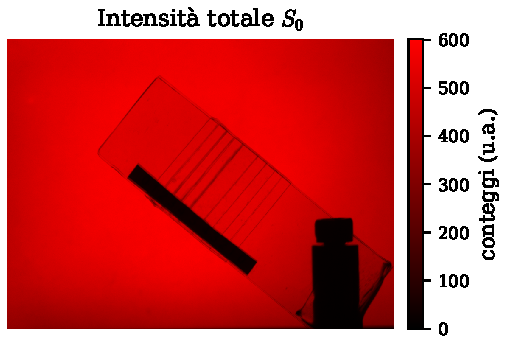
\includegraphics[height=0.205\textwidth]{Images/generated/strati_v2/R_S0.pdf}}\hfill
    \subfloat[Canale G ($\lambda_\mathrm{eff} \approx \SI{536}{\nano\meter}$)]{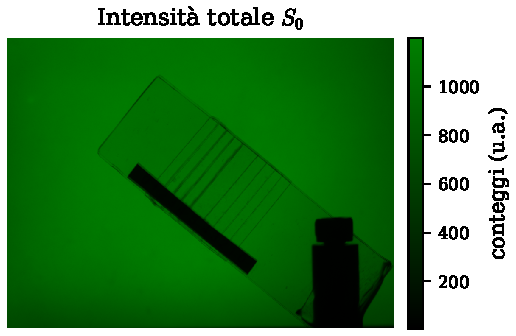
\includegraphics[height=0.205\textwidth]{Images/generated/strati_v2/G_S0.pdf}}\hfill
    \subfloat[Canale B ($\lambda_\mathrm{eff} \approx \SI{466}{\nano\meter}$)]{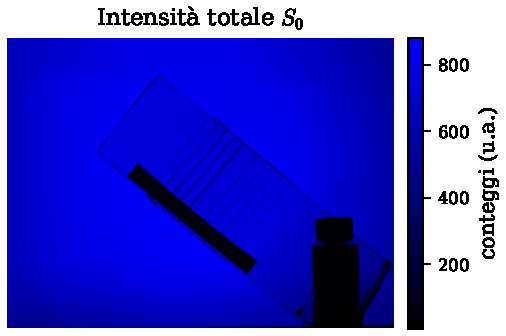
\includegraphics[height=0.205\textwidth]{Images/generated/strati_v2/B_S0.pdf}}
    \caption{Mappe di intensità $S_0$ del nastro adesivo stratificato sui tre canali del sensore. I gradini di spessore della pila simmetrica $1$-$2$-$3$-$4$-$5$-$4$-$3$-$2$-$1$ sono distinguibili come bande a diversa trasmissività.}
    \label{fig:nastro_s0}
\end{figure}

La mappa di ritardanza riflette direttamente la struttura a gradini, ma il valore letto in ciascuna banda è il residuo $\delta_\mathrm{vero} \bmod 360^\circ$: con un ritardo per strato prossimo a $\SI{240}{\degree}$, la successione dei valori misurati al crescere del numero di strati non è monotòna ma salta all'interno dell'intervallo $[0^\circ, 360^\circ)$ a ogni superamento del giro. L'istogramma della ritardanza sul campione presenta perciò un insieme discreto di picchi, uno per ciascun valore avvolto distinto, e la lettura strato per strato non è ricavabile dalla sola mappa. Per recuperare la ritardanza accumulata si ricorre all'analisi lungo una slice diagonale descritta nella \cref{sec:slice_dispersione}: una banda rettilinea spessa, orientata lungo la direzione di crescita della pila, viene campionata mediando circolarmente la ritardanza sulla larghezza, i plateau corrispondenti ai singoli strati vengono individuati per soglia sul gradiente ed etichettati da \texttt{1L} a \texttt{5} fino a \texttt{1R}, e un \emph{unwrap} cumulativo separato sul lato sinistro e destro ricostruisce la ritardanza vera prima dell'avvolgimento. Su questa si esegue il fit lineare attraverso l'origine $\delta = m\,n$.

Il canale rosso è il riferimento. La slice individua i nove plateau attesi (\cref{fig:nastro_slice_r}), con mediane che avvolgono da $\SI{247.6}{\degree}$ del primo strato fino a riavvolgersi più volte; l'istogramma in \cref{fig:nastro_hist_r} mostra la corrispondente struttura discreta dei valori avvolti sul campione. Dopo l'unwrap, i punti $(n, \delta)$ giacciono su una retta con pendenza $m_R = (240{,}2 \pm 0{,}9)~\si{\degree}$/strato (errore standard statistico del fit), coefficiente di determinazione $R^2 = 0{,}9994$ e scarto quadratico medio di $\SI{7.7}{\degree}$.

\begin{figure}[H]
    \centering
    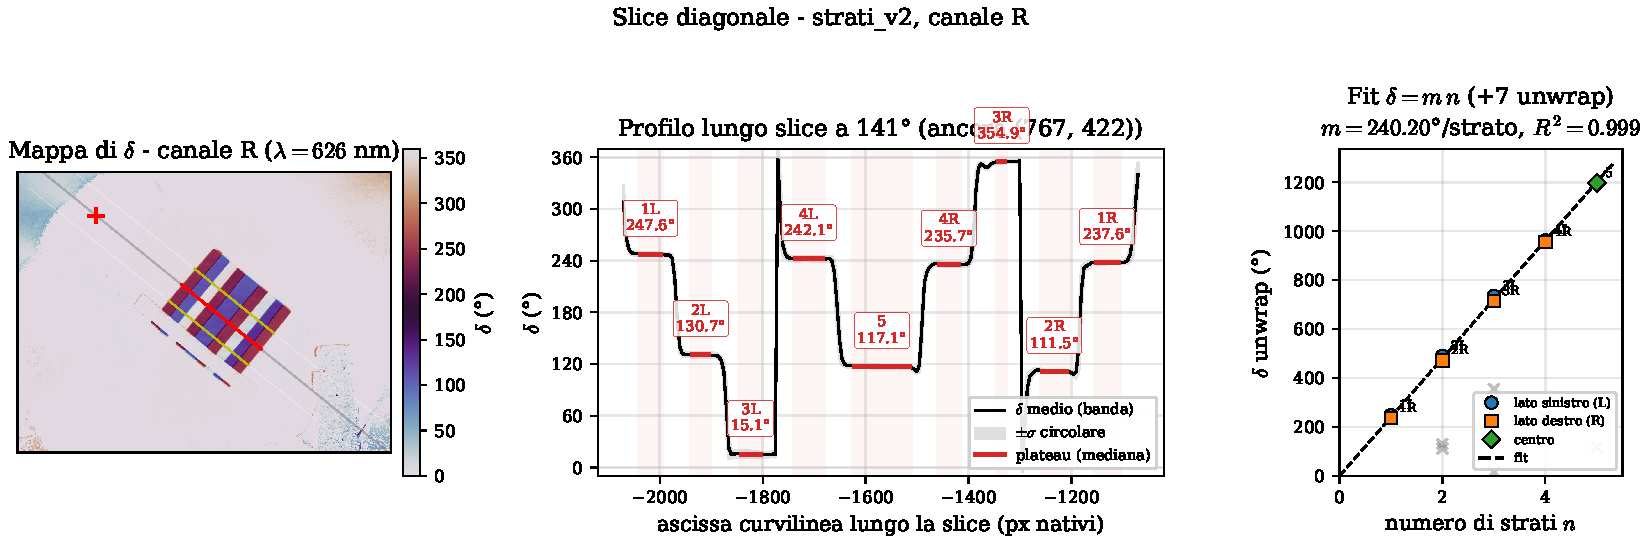
\includegraphics[width=\textwidth]{Images/generated/strati_v2/R_slice.pdf}
    \caption{Analisi della slice diagonale sul canale rosso. A sinistra la mappa di $\delta$ con la traccia della slice; al centro il profilo della ritardanza media lungo la slice con i plateau dei singoli strati evidenziati; a destra il fit lineare attraverso l'origine $\delta = m\,n$ dopo l'\emph{unwrap} cumulativo per lato.}
    \label{fig:nastro_slice_r}
\end{figure}

\begin{figure}[H]
    \centering
    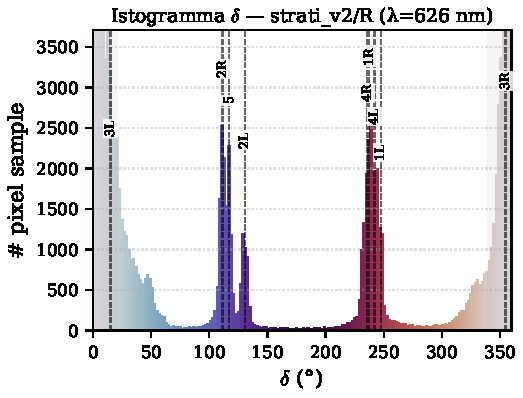
\includegraphics[width=0.62\textwidth]{Images/generated/strati_v2/R_hist_delta.pdf}
    \caption{Istogramma della ritardanza $\delta$ sul campione di nastro, canale rosso. Le linee verticali marcano le mediane dei plateau della slice, etichettate per strato; la distribuzione discreta riflette l'avvolgimento modulo $360^\circ$.}
    \label{fig:nastro_hist_r}
\end{figure}

Il canale verde (\cref{fig:nastro_slice_g,fig:nastro_hist_g}) ripete la procedura con un ritardo per strato maggiore, $m_G = (280{,}8 \pm 1{,}5)~\si{\degree}$/strato ($R^2 = 0{,}9988$, rms $\SI{12.9}{\degree}$), coerente con l'aumento atteso della ritardanza al diminuire della lunghezza d'onda.

\begin{figure}[H]
    \centering
    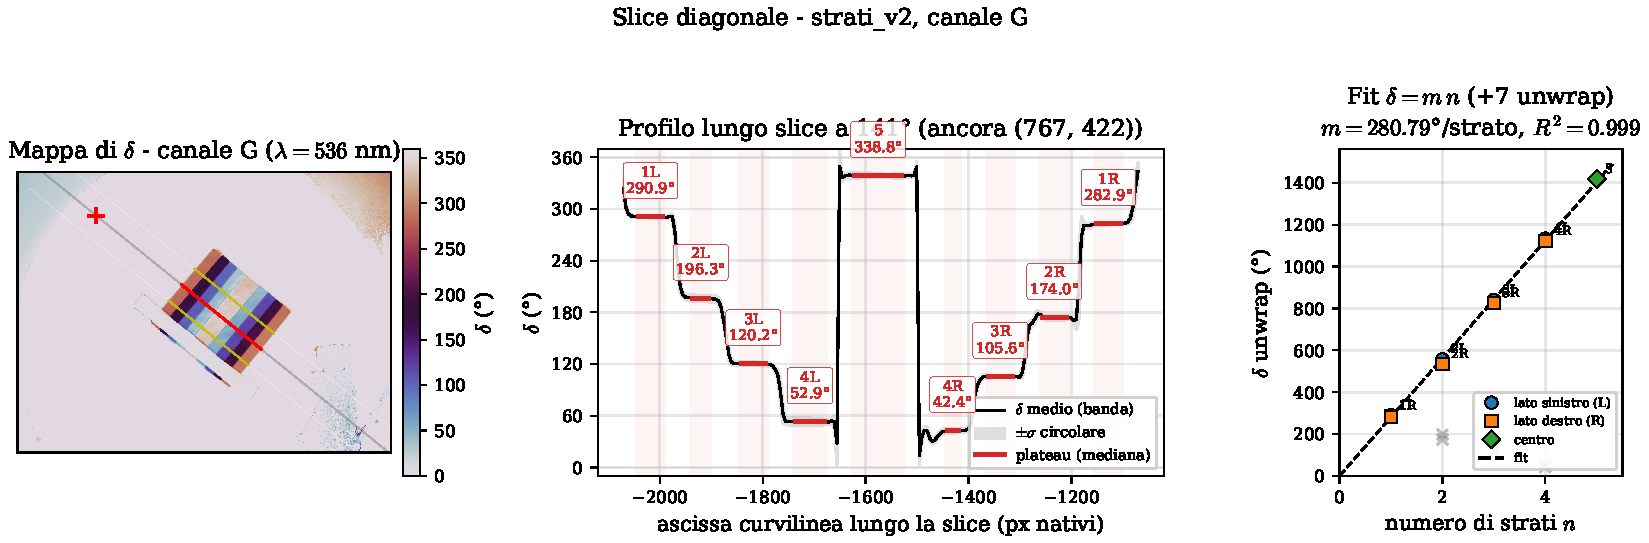
\includegraphics[width=\textwidth]{Images/generated/strati_v2/G_slice.pdf}
    \caption{Analisi della slice diagonale sul canale verde, con la stessa struttura a tre pannelli della \cref{fig:nastro_slice_r}.}
    \label{fig:nastro_slice_g}
\end{figure}

\begin{figure}[H]
    \centering
    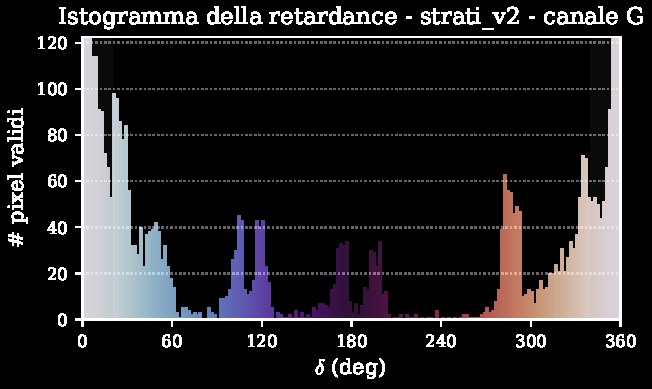
\includegraphics[width=0.62\textwidth]{Images/generated/strati_v2/G_hist_delta.pdf}
    \caption{Istogramma della ritardanza $\delta$ sul campione di nastro, canale verde, con le mediane dei plateau della slice.}
    \label{fig:nastro_hist_g}
\end{figure}

Il canale blu (\cref{fig:nastro_slice_b,fig:nastro_hist_b}) presenta il ritardo per strato più elevato, $m_B = (316{,}8 \pm 1{,}7)~\si{\degree}$/strato ($R^2 = 0{,}9987$, rms $\SI{14.8}{\degree}$); lo scarto quadratico medio cresce dal rosso al blu di pari passo con il peggioramento del rapporto segnale-rumore alle lunghezze d'onda corte.

\begin{figure}[H]
    \centering
    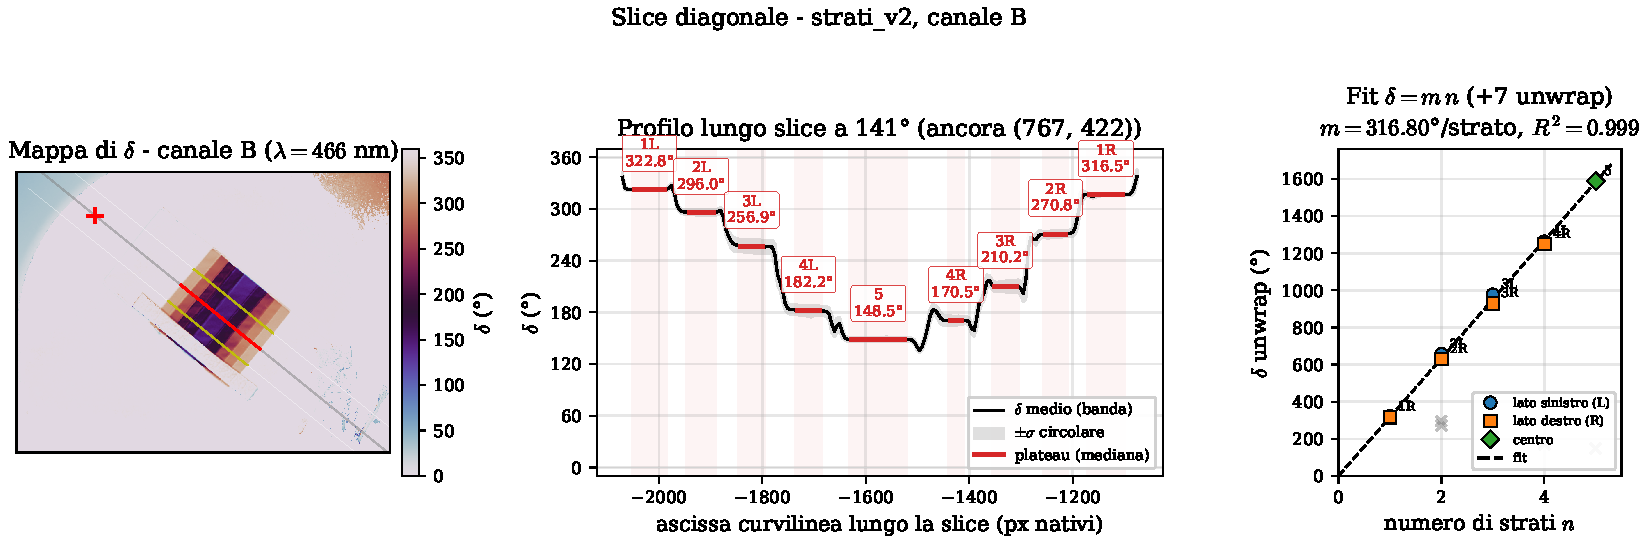
\includegraphics[width=\textwidth]{Images/generated/strati_v2/B_slice.pdf}
    \caption{Analisi della slice diagonale sul canale blu, con la stessa struttura a tre pannelli della \cref{fig:nastro_slice_r}.}
    \label{fig:nastro_slice_b}
\end{figure}

\begin{figure}[H]
    \centering
    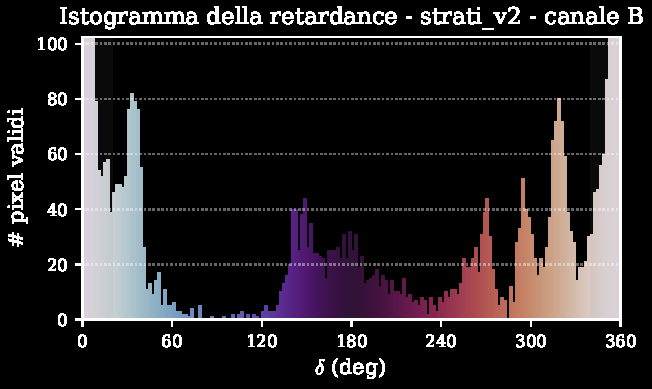
\includegraphics[width=0.62\textwidth]{Images/generated/strati_v2/B_hist_delta.pdf}
    \caption{Istogramma della ritardanza $\delta$ sul campione di nastro, canale blu, con le mediane dei plateau della slice.}
    \label{fig:nastro_hist_b}
\end{figure}

La \cref{tab:nastro_plateau} raccoglie le mediane di ritardanza dei nove plateau, così come misurate (avvolte in $[0^\circ, 360^\circ)$), per i tre canali; la non-monotonia delle colonne è la manifestazione diretta dell'avvolgimento. La \cref{tab:nastro_slope} riassume invece le pendenze ricavate dal fit lineare dopo l'unwrap.

\begin{table}[H]
    \centering
    \caption{Mediana della ritardanza $\delta$ misurata (avvolta in $[0^\circ, 360^\circ)$) per ciascun plateau della slice, sui tre canali. Le etichette indicano il numero di strati e il lato (L sinistro, R destro) rispetto al centro della pila.}
    \label{tab:nastro_plateau}
    \begin{tabular}{lccccccccc}
        \hline
        \textbf{Canale} & 1L & 2L & 3L & 4L & 5 & 4R & 3R & 2R & 1R \\
        \hline
        Rosso & $247{,}6$ & $130{,}7$ & $15{,}1$  & $242{,}1$ & $117{,}1$ & $235{,}7$ & $354{,}9$ & $111{,}5$ & $237{,}6$ \\
        Verde & $290{,}6$ & $196{,}6$ & $119{,}8$ & $53{,}5$  & $338{,}5$ & $42{,}9$  & $105{,}4$ & $173{,}9$ & $282{,}7$ \\
        Blu   & $321{,}2$ & $295{,}3$ & $258{,}5$ & $182{,}3$ & $147{,}2$ & $169{,}9$ & $212{,}1$ & $271{,}9$ & $315{,}2$ \\
        \hline
    \end{tabular}
\end{table}

\begin{table}[H]
    \centering
    \caption{Ritardo di fase per singolo strato di nastro adesivo, ricavato dal fit lineare attraverso l'origine $\delta = m\,n$ sui plateau della slice dopo \emph{unwrap}. L'incertezza su $m$ è l'errore standard statistico del fit sui nove plateau, ricavato dai residui; non include i contributi sistematici discussi nella \cref{sec:discussione}.}
    \label{tab:nastro_slope}
    \begin{tabular}{lcccc}
        \hline
        \textbf{Canale} & $\lambda_\mathrm{eff}$ [\si{\nano\meter}] & $m$ [\si{\degree}/strato] & $R^2$ & rms [\si{\degree}] \\
        \hline
        Rosso & 626 & $240{,}2 \pm 0{,}9$ & $0{,}9994$ & $7{,}7$  \\
        Verde & 536 & $280{,}8 \pm 1{,}5$ & $0{,}9988$ & $12{,}9$ \\
        Blu   & 466 & $316{,}8 \pm 1{,}7$ & $0{,}9987$ & $14{,}8$ \\
        \hline
    \end{tabular}
\end{table}

La linearità della risposta è eccellente su tutti e tre i canali, con $R^2 > 0{,}998$: il sistema ricostruisce una ritardanza accumulata fino a oltre $\SI{1500}{\degree}$ mantenendo la proporzionalità diretta con il numero di strati, una volta risolto l'avvolgimento tramite l'unwrap geometrico della slice. La simmetria della pila è rispettata entro pochi gradi sulla maggior parte dei plateau, confermando la coerenza spaziale della ricostruzione.

Il confronto delle regioni omologhe a tre strati evidenzia un'asimmetria residua fra lato sinistro e destro: contenuta sul rosso ($\SI{735.1}{\degree}$ contro $\SI{714.9}{\degree}$, $\SI{20.2}{\degree}$) e sul verde ($\SI{839.8}{\degree}$ contro $\SI{825.4}{\degree}$, $\SI{14.3}{\degree}$), essa sale a $\SI{46.4}{\degree}$ sul blu ($\SI{978.5}{\degree}$ contro $\SI{932.1}{\degree}$). L'effetto è confinato al terzo strato e al solo canale blu, non comparendo negli altri strati né sugli altri canali, ed è quindi incompatibile con un'asimmetria fisica generica del campione. Le verifiche condotte hanno escluso difetti di allineamento dei frame, depolarizzazione locale e asimmetrie nella distribuzione dei vettori di Stokes; la causa, plausibilmente una registrazione cromatica imperfetta del canale blu o un'interferenza sottile selettiva negli strati di adesivo, resta non identificata. Trattandosi di un'anomalia localizzata a un singolo punto, essa non influisce né sulla pendenza media né sulla linearità della risposta ($R^2 > 0{,}998$), entrambe ricavate dal fit complessivo sui nove plateau.

La dipendenza della ritardanza per strato dalla lunghezza d'onda è riassunta dai due grafici di \cref{fig:nastro_fit}. Il primo riporta i valori srotolati di $\delta$ in funzione del numero di strati per i tre canali, con le rispettive rette di fit attraverso l'origine; il secondo riporta le tre pendenze $m_c$ in funzione della lunghezza d'onda, con il fit di dispersione $m(\lambda) = k/\lambda$. Il fit restituisce $k = (1{,}492 \pm 0{,}010)\cdot10^{5}~\si{\degree\nano\meter}$/strato con $R^2 = 0{,}993$, dove l'incertezza è l'errore standard statistico del fit. Il rapporto fra le pendenze agli estremi spettrali, $m_B/m_R = 316{,}8/240{,}2 = 1{,}319$, è leggermente inferiore al rapporto puramente geometrico $\lambda_R/\lambda_B = 626/466 = 1{,}343$. La decomposizione per canale chiarisce la natura dello scarto: il prodotto $m \cdot \lambda$, costante per una dispersione puramente geometrica, coincide fra rosso e verde entro lo $0{,}1\%$, mentre il blu risulta inferiore dell'$1{,}8\%$. Una dispersione normale della birifrangenza, con $\Delta n$ crescente verso il blu come atteso per un polimero stirato, sposterebbe il rapporto nella direzione opposta; lo scarto, di segno contrario e confinato al solo canale blu, è dunque da attribuire a un residuo sistematico di quel canale, lo stesso interessato dall'anomalia locale discussa sopra, piuttosto che a una proprietà del materiale. L'effetto, dell'ordine del punto percentuale, non incide sulla linearità della risposta.

\begin{figure}[H]
    \centering
    \subfloat[Ritardanza srotolata in funzione del numero di strati, tre canali, con fit lineare attraverso l'origine.]{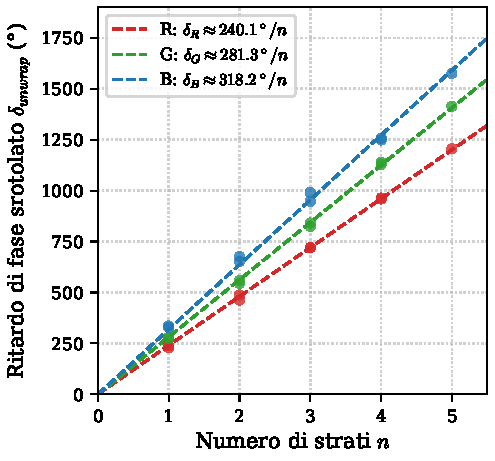
\includegraphics[width=0.46\textwidth]{Images/generated/strati_fit/fit_strati_linear.pdf}}\hfill
    \subfloat[Pendenza per strato in funzione della lunghezza d'onda, con fit di dispersione $m(\lambda) = k/\lambda$.]{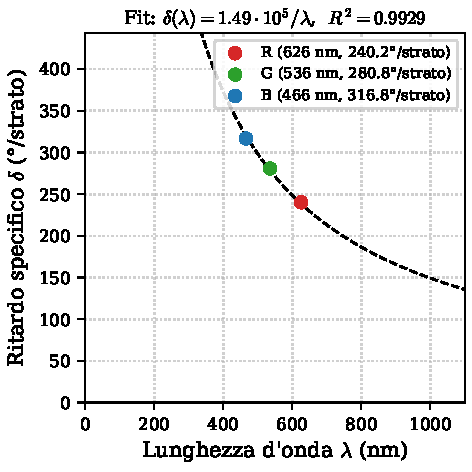
\includegraphics[width=0.46\textwidth]{Images/generated/strati_fit/fit_lambda_inverse.pdf}}
    \caption{Dipendenza spettrale della ritardanza del nastro adesivo. A sinistra la linearità $\delta = m\,n$ sui tre canali; a destra la dispersione delle pendenze, ben descritta dalla legge $m \propto 1/\lambda$ propria di un materiale a birifrangenza debolmente dispersiva.}
    \label{fig:nastro_fit}
\end{figure}

% ---------------------------------------------------------------------------
\section{Versatilità del sistema}
\label{sec:risultati_versatilita}

Dopo aver verificato che il polarimetro produce mappe coerenti per campioni birifrangenti, si passa a fenomeni fisicamente distinti per dimostrare la generalità del metodo.

\subsection{Soluzione di saccarosio}
\label{subsec:soluzione_zucchero}

La soluzione di saccarosio in acqua è otticamente attiva: il saccarosio destrogiro ruota il piano di polarizzazione della luce trasmessa di un angolo proporzionale al cammino ottico e alla concentrazione. A differenza della birifrangenza, l'attività ottica agisce sulle sole componenti lineari $S_1$ e $S_2$ senza coinvolgere $S_3$, e si manifesta come una rotazione rigida e spazialmente uniforme dell'angolo di polarizzazione lineare. La soluzione è contenuta in una boccetta a facce piane parallele di spessore interno $L = \SI{13}{\milli\meter}$; lo sfondo libero, allineato a $\mathrm{AoLP} \approx \SI{0}{\degree}$ per costruzione (\cref{sec:allineamento}), fornisce il riferimento rispetto al quale si misura la rotazione. Nella convenzione adottata (\cref{subsec:stokes_def}) una rotazione destrogira corrisponde a un AoLP negativo: la misura restituisce infatti un AoLP del cluster della soluzione sistematicamente negativo, da $-3{,}95^\circ$ al rosso a $-6{,}12^\circ$ al blu, in accordo con il carattere destrogiro del saccarosio e come conferma sperimentale indipendente della convenzione di segno. Nel seguito si indica con $\psi = |\mathrm{AoLP}|$ il modulo di tale rotazione, impiegato nella legge di Biot con il potere rotatorio specifico tabulato $[\alpha] > 0$ (convenzione chimica per le sostanze destrogire).

\begin{figure}[H]
    \centering
    \subfloat[Canale R ($\lambda_\mathrm{eff} \approx \SI{626}{\nano\meter}$)]{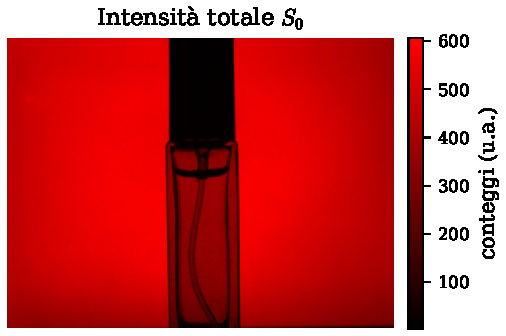
\includegraphics[height=0.205\textwidth]{Images/generated/zucchero/R_S0.pdf}}\hfill
    \subfloat[Canale G ($\lambda_\mathrm{eff} \approx \SI{536}{\nano\meter}$)]{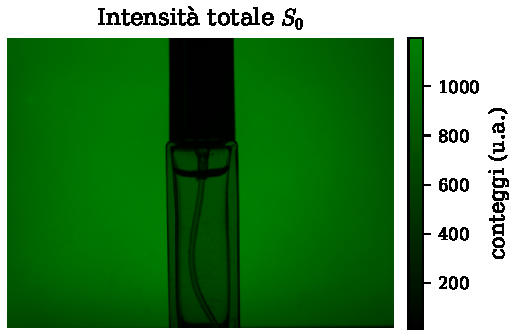
\includegraphics[height=0.205\textwidth]{Images/generated/zucchero/G_S0.pdf}}\hfill
    \subfloat[Canale B ($\lambda_\mathrm{eff} \approx \SI{466}{\nano\meter}$)]{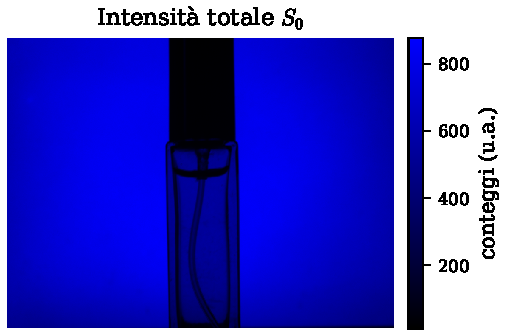
\includegraphics[height=0.205\textwidth]{Images/generated/zucchero/B_S0.pdf}}
    \caption{Mappe di intensità $S_0$ della soluzione di saccarosio sui tre canali del sensore. Si distinguono la boccetta con la soluzione e la cannuccia in plastica impiegata nella preparazione, che introduce una birifrangenza da stress propria visibile localmente nelle mappe di polarizzazione.}
    \label{fig:zucchero_s0}
\end{figure}

La rotazione ottica è piccola, dell'ordine di pochi gradi, e la regione utile della soluzione va distinta dallo sfondo e dai contributi spuri della cannuccia e delle pareti di vetro della boccetta; le eventuali tensioni residue del vetro introdurrebbero peraltro una birifrangenza locale, ossia $\delta \neq 0$, e non una rotazione uniforme dell'AoLP, e non possono quindi mimare l'attività ottica. La stima viene quindi affidata alla procedura di clustering non parziale descritta nella \cref{sec:umap_clustering}, applicata questa volta all'angolo di polarizzazione lineare: l'embedding UMAP dei descrittori di Stokes viene segmentato con HDBSCAN, e il cluster vincente (quello che combina dimensione apprezzabile, bassa dispersione angolare interna e distanza angolare significativa dal cluster dominante dello sfondo) identifica i pixel della soluzione, restituendone l'AoLP mediano, il cui modulo $\tilde\psi_{\mathrm{win}} = |\mathrm{AoLP}|$ quantifica la rotazione ottica. La procedura è ripetuta sui tre canali (\cref{fig:zucchero_winner_r,fig:zucchero_winner_g,fig:zucchero_winner_b}), fornendo tre stime indipendenti alle rispettive lunghezze d'onda; la deviazione mediana assoluta dell'AoLP entro il cluster vincente è inferiore a $0{,}5^\circ$ su tutti i canali.

\begin{figure}[H]
    \centering
    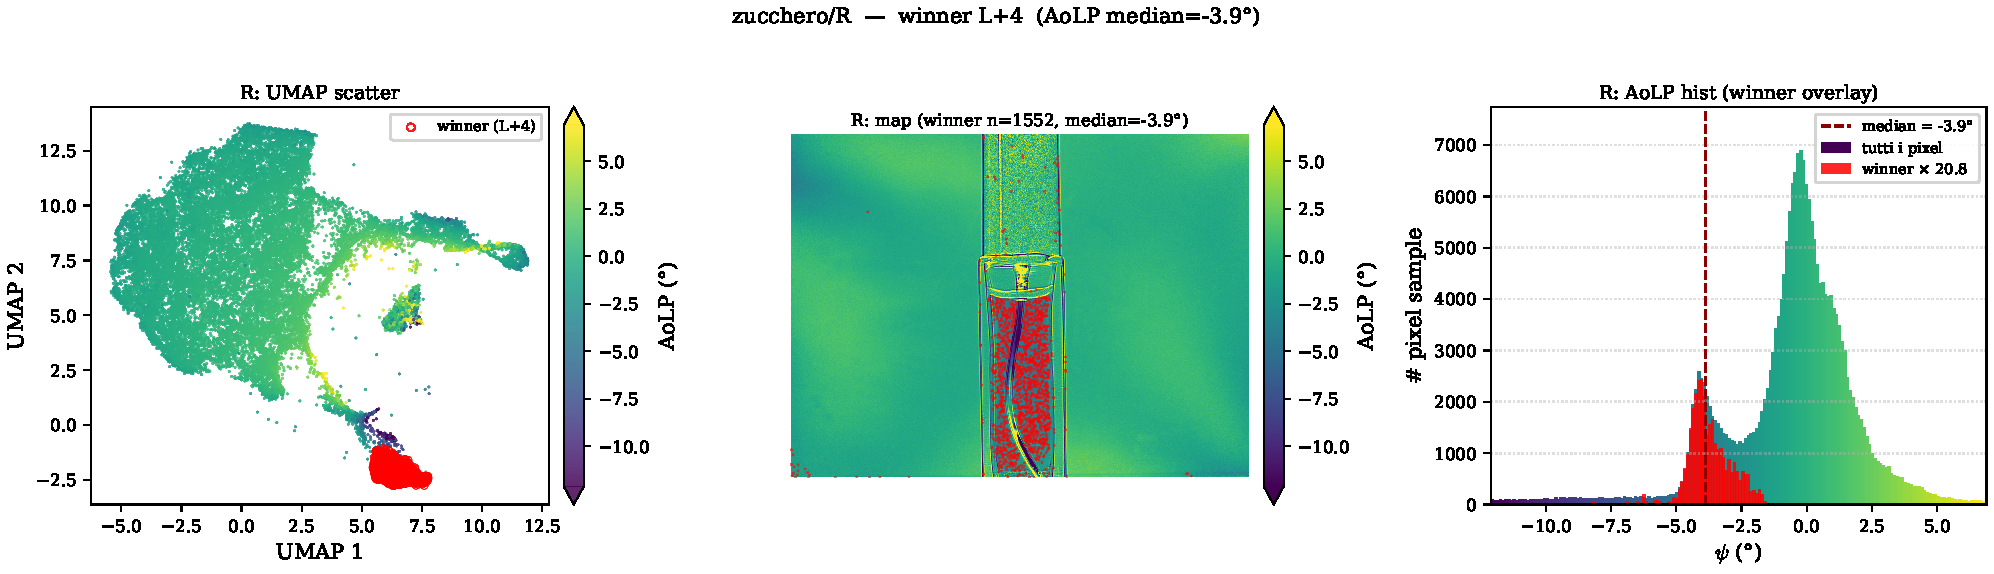
\includegraphics[width=\textwidth]{Images/generated/zucchero/R_aolp_winner.pdf}
    \caption{Identificazione del cluster vincente sul canale rosso: embedding UMAP colorato per AoLP (sinistra), mappa spaziale con il cluster della soluzione evidenziato (centro) e istogramma dell'AoLP (destra). La mediana del cluster vincente è $\mathrm{AoLP} = -3{,}95^\circ$ (rotazione destrogira), corrispondente a una rotazione ottica di modulo $\tilde\psi_{\mathrm{win}} = \SI{3.95}{\degree}$.}
    \label{fig:zucchero_winner_r}
\end{figure}

\begin{figure}[H]
    \centering
    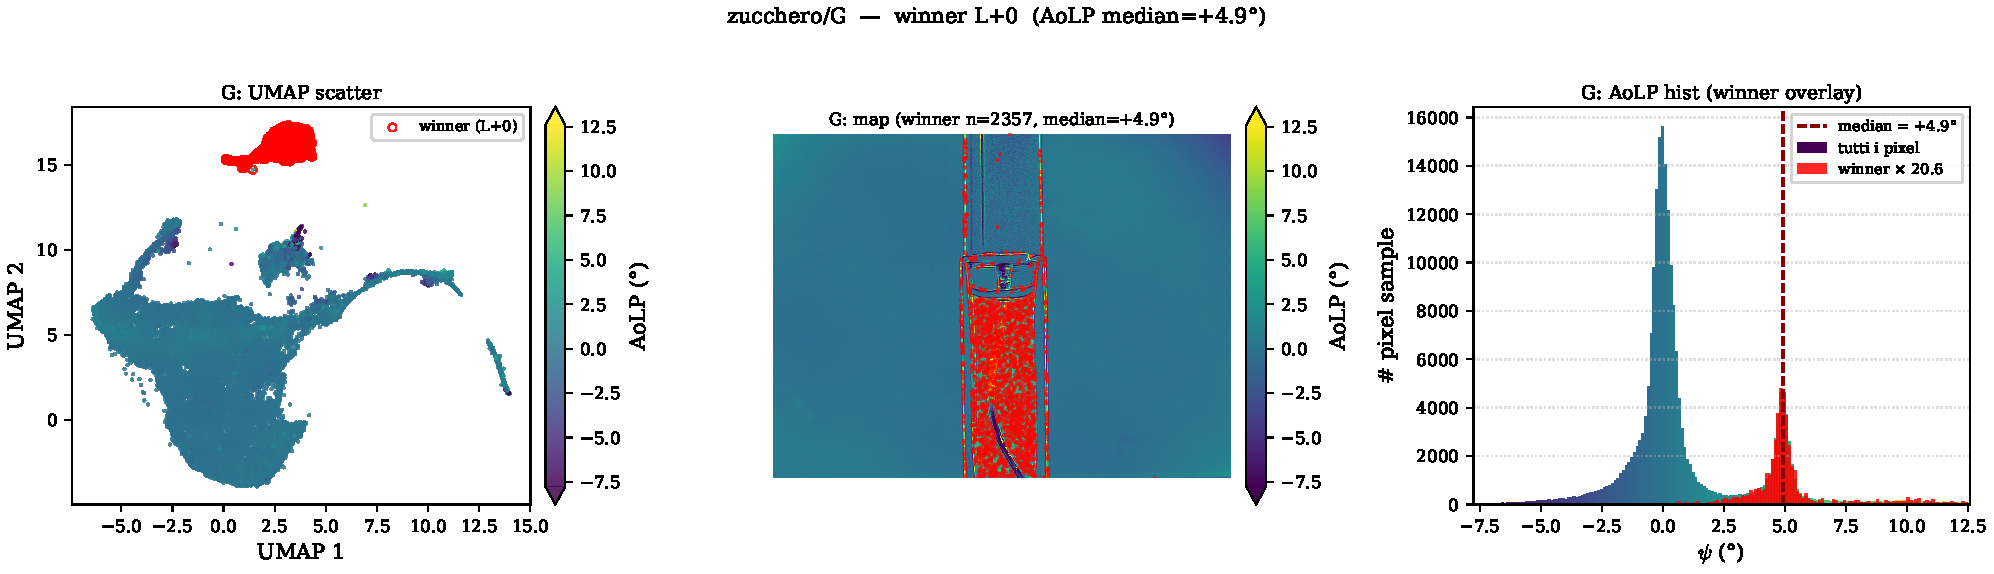
\includegraphics[width=\textwidth]{Images/generated/zucchero/G_aolp_winner.pdf}
    \caption{Cluster vincente sul canale verde, con la stessa struttura a tre pannelli della \cref{fig:zucchero_winner_r}. L'AoLP mediano è $-4{,}92^\circ$, ossia una rotazione di modulo $\tilde\psi_{\mathrm{win}} = \SI{4.92}{\degree}$.}
    \label{fig:zucchero_winner_g}
\end{figure}

\begin{figure}[H]
    \centering
    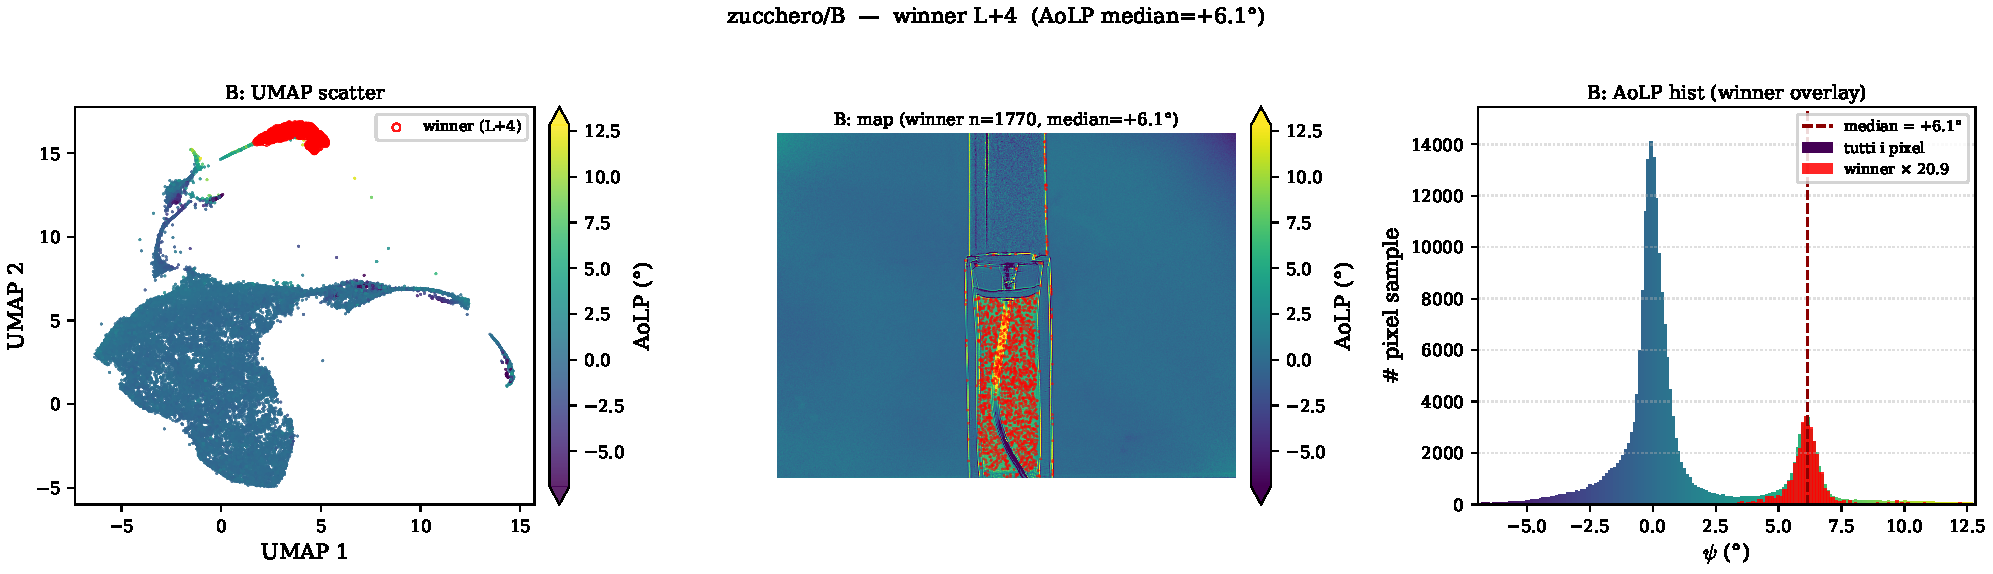
\includegraphics[width=\textwidth]{Images/generated/zucchero/B_aolp_winner.pdf}
    \caption{Cluster vincente sul canale blu, con la stessa struttura a tre pannelli della \cref{fig:zucchero_winner_r}. L'AoLP mediano è $-6{,}12^\circ$, ossia una rotazione di modulo $\tilde\psi_{\mathrm{win}} = \SI{6.12}{\degree}$, la più ampia dei tre canali.}
    \label{fig:zucchero_winner_b}
\end{figure}

La rotazione cresce in modulo al diminuire della lunghezza d'onda, da $\SI{3.95}{\degree}$ al rosso a $\SI{6.12}{\degree}$ al blu, manifestazione della dispersione rotatoria ottica. Il fit con il modello di Drude semplificato, eseguito sull'AoLP mediano con il proprio segno, $\mathrm{AoLP}(\lambda) = k/\lambda^2$ (\cref{fig:zucchero_fit}), restituisce $k = (-1{,}390 \pm 0{,}056)\cdot10^{6}~\si{\degree\nano\meter\squared}$ (errore standard statistico) con $R^2 = 0{,}90$, coerente con $\psi(\lambda) = |k|/\lambda^2$: il modulo di $k$ descrive la dispersione rotatoria, il segno negativo la rotazione destrogira. Il rapporto fra i moduli agli estremi spettrali, $|\psi_B|/|\psi_R| = 6{,}12/3{,}95 = 1{,}55$, è inferiore al rapporto $(\lambda_R/\lambda_B)^2 = 1{,}80$ atteso dal modello $1/\lambda^2$ puro: la dispersione misurata è più piatta della legge inversa quadratica, con uno scostamento che cresce in modo regolare verso le lunghezze d'onda corte. La risonanza ultravioletta del saccarosio non può esserne la causa, poiché renderebbe la dispersione più ripida della legge $1/\lambda^2$, non più piatta; l'appiattimento è quindi da attribuire ai residui sistematici della misura, crescenti verso il blu dove il rapporto segnale-rumore peggiora, e si riflette coerentemente nella lieve decrescita monotona delle stime di concentrazione per canale (\cref{tab:zucchero_conc}).

\begin{figure}[H]
    \centering
    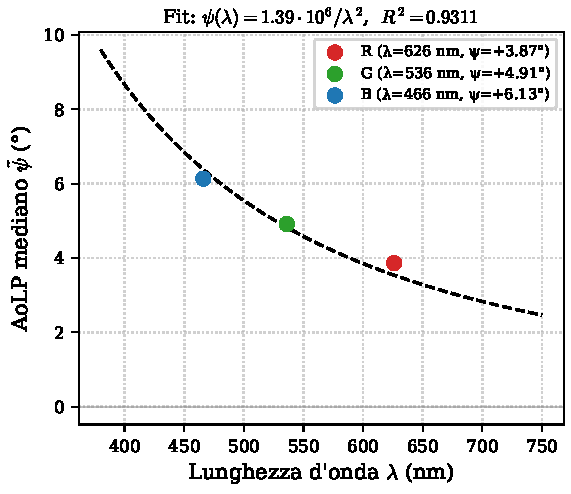
\includegraphics[width=0.55\textwidth]{Images/generated/zucchero/aolp_lambda_fit.pdf}
    \caption{Fit di dispersione rotatoria $\mathrm{AoLP}(\lambda) = k/\lambda^2$ (modello di Drude semplificato, con segno) sull'AoLP mediano del cluster vincente. I punti colorati sono l'AoLP per canale alle rispettive $\lambda_\mathrm{eff}$, con segno negativo coerente con il carattere destrogiro del saccarosio; la curva tratteggiata è il fit non lineare ai minimi quadrati.}
    \label{fig:zucchero_fit}
\end{figure}

La rotazione misurata permette una stima della concentrazione tramite la legge di Biot, $\psi = [\alpha]_\lambda\,L\,c$, dove $[\alpha]_\lambda$ è il potere rotatorio specifico del saccarosio, $L$ il cammino ottico e $c$ la concentrazione in massa per unità di volume. Le misure sono state condotte a temperatura ambiente, non registrata: la dipendenza termica del potere rotatorio del saccarosio è debole, e la sua variazione su pochi gradi attorno alla temperatura di riferimento resta ampiamente al di sotto degli scarti osservati fra i canali. Il valore tabulato alla riga D del sodio, $[\alpha]_{589} = +66{,}5~\si{\degree}\,\si{\milli\liter}\,\si{\gram}^{-1}\,\si{\deci\meter}^{-1}$, viene riportato alle lunghezze d'onda di lavoro tramite lo stesso scaling di Drude, $[\alpha]_\lambda = [\alpha]_{589}\,(589/\lambda)^2$. Invertendo la legge di Biot con $L = \SI{0.13}{\deci\meter}$ si ottengono le tre stime di concentrazione raccolte nella \cref{tab:zucchero_conc}.

\begin{table}[H]
    \centering
    \caption{Rotazione ottica del cluster vincente, potere rotatorio specifico riportato alla lunghezza d'onda di lavoro e concentrazione stimata via legge di Biot per la soluzione di saccarosio ($L = \SI{13}{\milli\meter}$).}
    \label{tab:zucchero_conc}
    \begin{tabular}{lcccc}
        \hline
        \textbf{Canale} & $\lambda_\mathrm{eff}$ [\si{\nano\meter}] & $\tilde\psi_{\mathrm{win}}$ [\si{\degree}] & $[\alpha]_\lambda$ [\si{\degree}\,\si{\milli\liter}\,\si{\gram}$^{-1}$\,\si{\deci\meter}$^{-1}$] & $c$ [\si{\gram\per\milli\liter}] \\
        \hline
        Rosso & 626 & $3{,}95$ & $58{,}9$  & $0{,}52$ \\
        Verde & 536 & $4{,}92$ & $80{,}3$  & $0{,}47$ \\
        Blu   & 466 & $6{,}12$ & $106{,}2$ & $0{,}44$ \\
        \hline
    \end{tabular}
\end{table}

Le tre stime si collocano entro circa il $\pm 9\%$ attorno al valore medio $c_\mathrm{ott} \approx \SI{0.47}{\gram\per\milli\liter}$, con la decrescita monotona dal rosso al blu già ricondotta ai residui sistematici della misura. La consistenza della concentrazione ricavata indipendentemente da tre canali colore distinti, ciascuno con la propria correzione di dispersione, è il risultato significativo della misura: il sistema recupera un valore quantitativo coerente combinando la legge di Biot con la dispersione rotatoria. La soluzione è stata preparata mescolando zucchero e acqua senza un controllo gravimetrico accurato, per cui non è disponibile un riferimento di concentrazione affidabile con cui validare l'accuratezza assoluta; il valore ricavato è comunque del tutto plausibile per una soluzione zuccherina concentrata e dimostra la capacità del polarimetro di misurare l'attività ottica in modo quantitativo e spettralmente coerente.

\subsection{Trave a sbalzo}
\label{subsec:risultati_cantilever}

La fotoelasticità è la comparsa di birifrangenza in un materiale otticamente isotropo sottoposto a sforzo meccanico: gli assi della birifrangenza indotta si allineano con le direzioni principali dello sforzo e il ritardo è proporzionale alla differenza degli sforzi principali. Il campione è una barra in materiale polimerico trasparente a sezione quadrata di lato $\SI{8}{\milli\meter}$, vincolata a un'estremità come trave a sbalzo e caricata all'estremità libera con un parallelepipedo metallico di massa circa $\SI{900}{\gram}$, corrispondente a una forza applicata dell'ordine di $\SI{9}{\newton}$; la distanza fra il punto di applicazione del carico e l'estremo del vincolo è di circa $\SI{73}{\milli\meter}$. Questi dati geometrici sono riportati a titolo di contesto e non vengono impiegati per un'analisi quantitativa. Le acquisizioni sono state ripetute nelle due condizioni di trave scarica (\texttt{barraoff\_v2}) e sotto carico (\texttt{barraon\_v2}).

L'orientazione del campione condiziona fortemente la leggibilità del segnale. La barra è stata posizionata con il proprio asse longitudinale parallelo alla direzione di polarizzazione della luce incidente; poiché in una trave inflessa lo sforzo principale è diretto lungo l'asse, gli assi della birifrangenza indotta risultano quasi paralleli (o perpendicolari) alla polarizzazione di ingresso. In questa configurazione l'angolo $\alpha$ fra asse veloce e polarizzazione è prossimo a $0^\circ$, e la conversione della polarizzazione lineare in componente circolare, governata dal fattore $\sin 2\alpha\,\sin\delta$ (\cref{eq:s3_ritardatore}), è fortemente soppressa. La stessa condizione rende degenere l'estrazione della ritardanza, che il peso di stabilità della pipeline (\cref{subsec:ambiguita_numeriche}) spinge verso zero quando $\sin^2 2\alpha \to 0$. Gli effetti birifrangenti sono perciò poco evidenti e l'estrazione di grandezze quantitative non è affidabile. Anche disponendo della geometria della barra, il modulo elastico del polimero e il coefficiente fotoelastico del materiale non sono noti, e l'orientazione sfavorevole rispetto alla polarizzazione sopprime comunque il segnale: per queste ragioni non si tenta una stima del campo di sforzo e l'analisi resta qualitativa, concentrandosi sulla componente $S_3$.

\begin{figure}[H]
    \centering
    \subfloat[Canale R ($\lambda_\mathrm{eff} \approx \SI{626}{\nano\meter}$)]{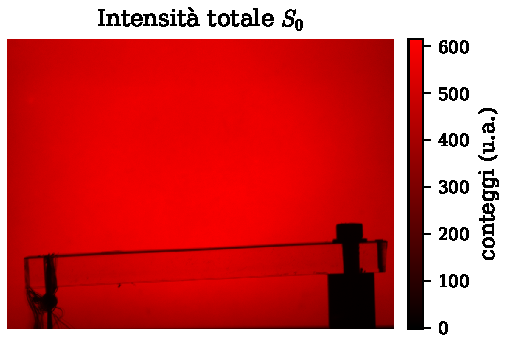
\includegraphics[height=0.205\textwidth]{Images/generated/barraon_v2/R_S0.pdf}}\hfill
    \subfloat[Canale G ($\lambda_\mathrm{eff} \approx \SI{536}{\nano\meter}$)]{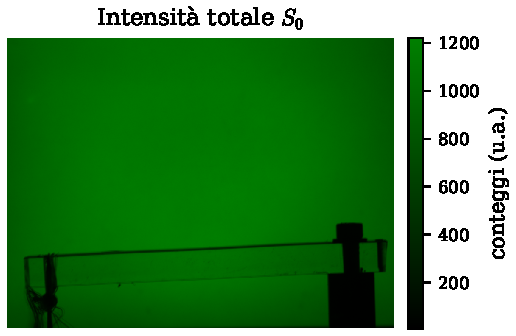
\includegraphics[height=0.205\textwidth]{Images/generated/barraon_v2/G_S0.pdf}}\hfill
    \subfloat[Canale B ($\lambda_\mathrm{eff} \approx \SI{466}{\nano\meter}$)]{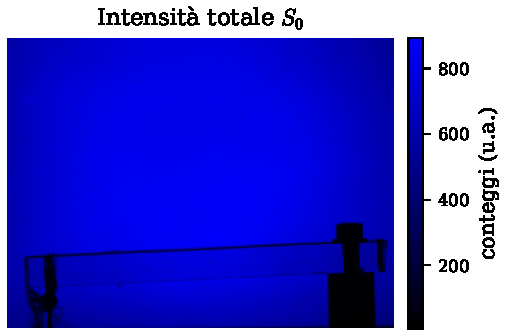
\includegraphics[height=0.205\textwidth]{Images/generated/barraon_v2/B_S0.pdf}}
    \caption{Mappe di intensità $S_0$ della trave a sbalzo sotto carico sui tre canali del sensore. Si distinguono il corpo della barra, il vincolo a sinistra e il supporto destro impiegato come riferimento per la registrazione.}
    \label{fig:barra_s0}
\end{figure}

Per isolare la variazione indotta dal carico, le acquisizioni con e senza peso vanno riportate alla stessa geometria: la trave sotto carico si flette e il campo di vista subisce un piccolo spostamento rigido fra le due riprese. Si applica perciò la procedura descritta nella \cref{sec:fotoelasticita}: un allineamento globale per correlazione di fase calcolato sul solo supporto destro, dove la flessione è trascurabile, seguito da una deformazione colonna-per-colonna che riporta la centerline della trave carica su quella della trave scarica. La mappa differenziale $\Delta S_3 = S_3^{\mathrm{on,\,warped}} - S_3^{\mathrm{off}}$, calcolata indipendentemente sui tre canali (\cref{fig:barra_ds3}), elimina la componente comune dovuta all'illuminazione e alla geometria, isolando il solo contributo dello stato di sforzo.

\begin{figure}[H]
    \centering
    \subfloat[Canale R]{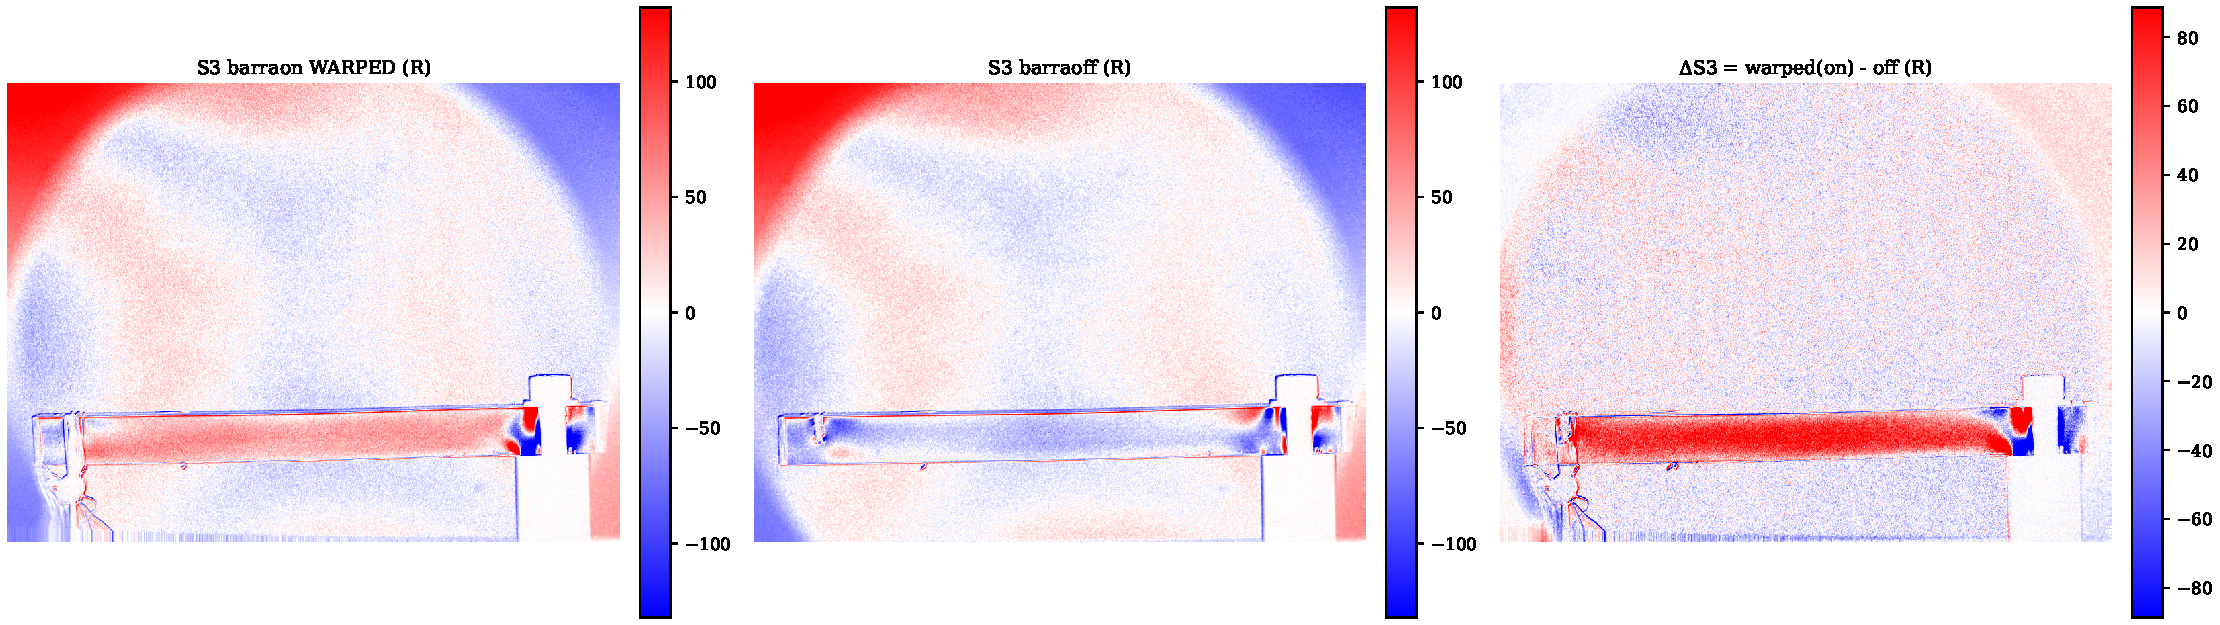
\includegraphics[height=0.205\textwidth]{Images/generated/barraon_v2/R_diff_s3_warped.pdf}}\hfill
    \subfloat[Canale G]{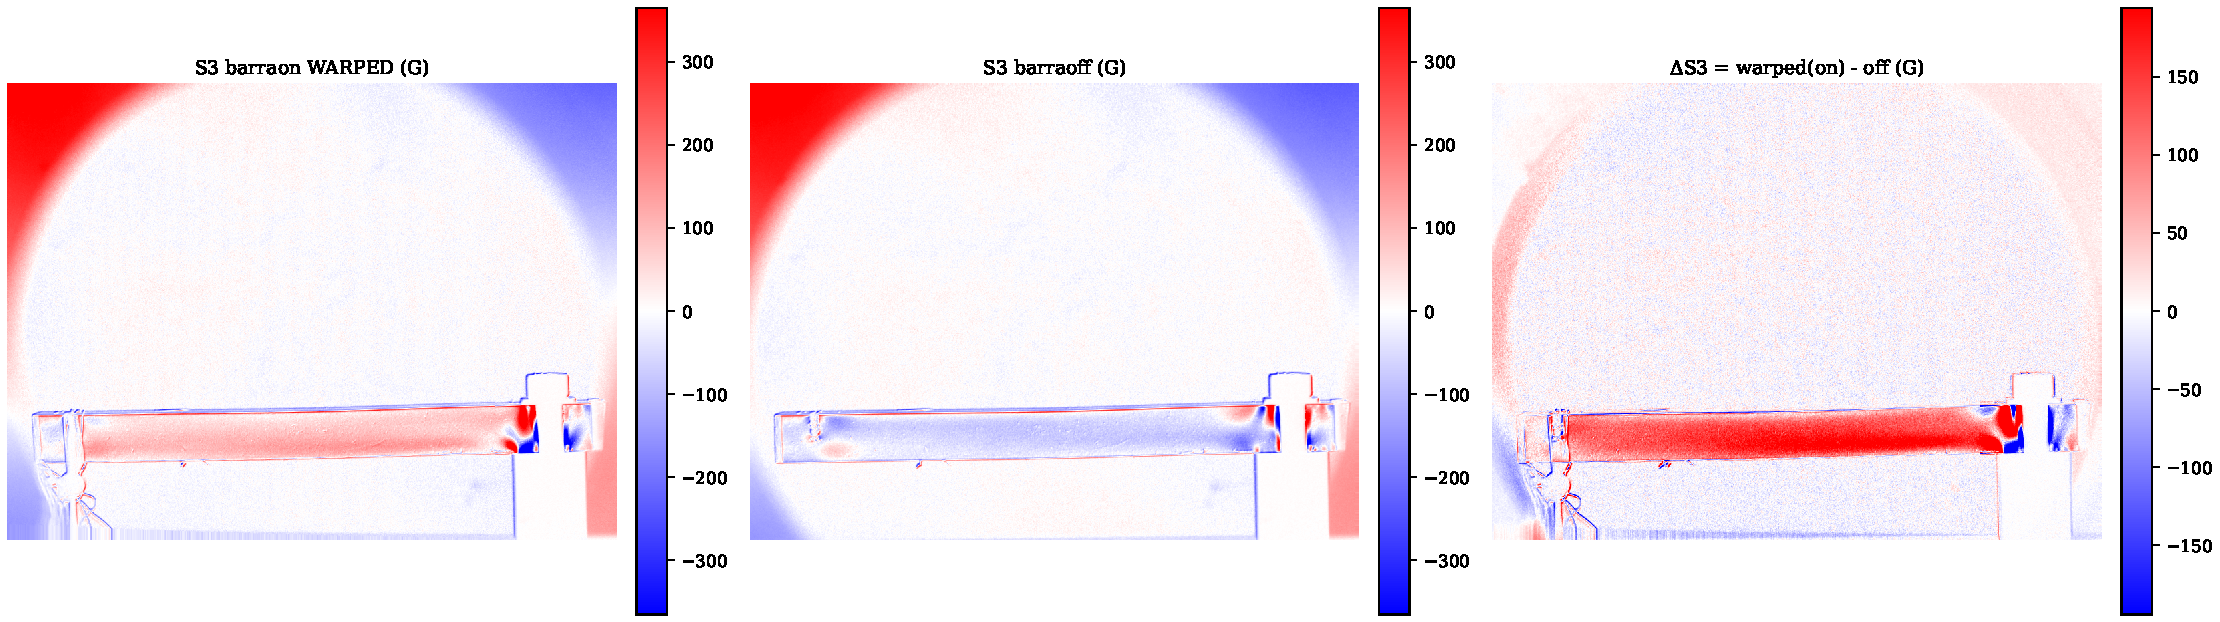
\includegraphics[height=0.205\textwidth]{Images/generated/barraon_v2/G_diff_s3_warped.pdf}}\hfill
    \subfloat[Canale B]{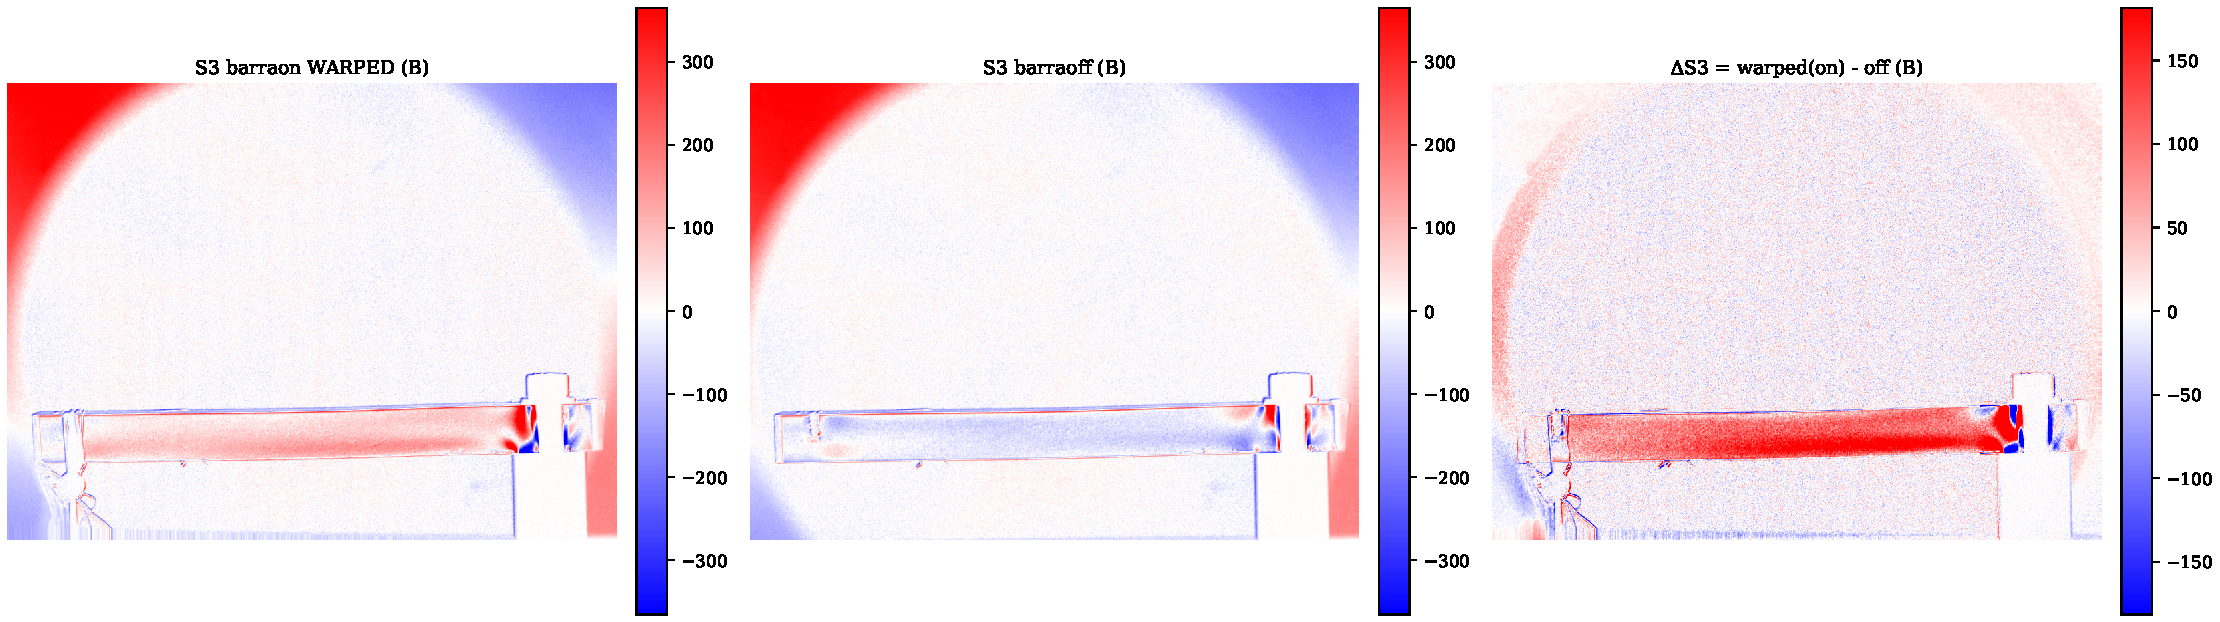
\includegraphics[height=0.205\textwidth]{Images/generated/barraon_v2/B_diff_s3_warped.pdf}}
    \caption{Mappa differenziale $\Delta S_3 = S_3^{\mathrm{on,\,warped}} - S_3^{\mathrm{off}}$ fra trave carica e scarica, sui tre canali del sensore, dopo registrazione e deformazione colonna-per-colonna. Il differenziale isola il contributo della birifrangenza indotta dal carico.}
    \label{fig:barra_ds3}
\end{figure}

% TODO (utente): inserire la lettura qualitativa specifica delle mappe DeltaS3 (dove compare il segnale sotto carico, segno, eventuale localizzazione presso il vincolo). Confine di interpretazione umana: la descrizione spaziale delle mappe spetta all'utente.
La mappa differenziale evidenzia, sia pur debolmente, la comparsa di un segnale $S_3$ associato al carico, assente nella configurazione scarica: il confronto conferma in via qualitativa la natura fotoelastica del campione e la sensibilità del polarimetro alla birifrangenza indotta da sforzo, pur nei limiti imposti dall'orientazione sfavorevole della barra rispetto alla polarizzazione incidente.

% ---------------------------------------------------------------------------
\section{Discussione}
\label{sec:discussione}

I risultati presentati nelle sezioni precedenti dimostrano che il sistema è in grado di ricostruire il vettore di Stokes completo con risoluzione spaziale bidimensionale, di misurare ritardanza e asse veloce su campioni macroscopici, e di distinguere fenomeni polarimetrici di natura diversa (birifrangenza, attività ottica, fotoelasticità) con un apparato il cui costo complessivo, escluso lo smartphone, è inferiore a 100\,\texteuro.

Una stima rigorosa dell'incertezza di misura esula dalle possibilità di questo lavoro: quantificarla richiederebbe una calibrazione dello strumento contro campioni a ritardanza nota e con incertezza certificata, riferimenti non disponibili per un prototipo che non ha ancora ricevuto una caratterizzazione metrologica. In assenza di tali standard, l'accuratezza può essere valutata soltanto per confronto con le previsioni teoriche sui campioni di validazione, e gli scarti osservati si collocano nell'ordine di pochi gradi. Le incertezze riportate sui parametri dei fit (la pendenza per strato del nastro e i prefattori di dispersione) sono errori standard puramente statistici, ricavati dai residui dei fit stessi: quantificano la riproducibilità interna dei dati, non l'accuratezza assoluta, che resta dominata dai contributi sistematici discussi in questa sezione. La lamina quarto d'onda, il cui ritardo misurato è stato confrontato con la legge di dispersione di un ritardatore a singolo ordine (\cref{subsec:risultati_qw}), ne è l'esempio più diretto: lo scarto è di pochi gradi al rosso, prossimo al punto di design, mentre l'eccedenza che cresce verso il blu ingloba anche il contributo fisico della dispersione del materiale, che il riferimento puramente geometrico per costruzione non modella. Tali valori vanno intesi come ordine di grandezza dell'accordo con la teoria, non come una barra d'errore calibrata.

Lo scarto non si distribuisce in modo uniforme fra le grandezze ricostruite, e la gerarchia osservata riflette la lunghezza della catena di misura che ciascuna richiede. L'angolo di polarizzazione lineare e il grado di polarizzazione discendono direttamente dai parametri di Stokes lineari $S_0$, $S_1$ e $S_2$, estratti dal sistema sovradeterminato delle trentasei acquisizioni angolari, e risultano perciò le grandezze più stabili. La ritardanza richiede invece la determinazione di $S_3$, e con essa le due acquisizioni aggiuntive con lamina $\lambda/4$, la correzione cromatica del ritardo della lamina e l'azzeramento dell'ellitticità residua sulla sfera di Poincaré; la catena più lunga, sommata all'ambiguità di avvolgimento modulo $360^\circ$ per i campioni ad alta ritardanza, rende $\delta$ la quantità intrinsecamente meno precisa, in accordo con la maggiore sensibilità del suo calcolo alle approssimazioni discusse di seguito.

% TODO: check (coerenza downsample f=4 sistemata da AI 2026-05-21)
Il principale compromesso è introdotto dal downsampling: con il fattore $f = 4$ adottato in questo lavoro la risoluzione di analisi resta di circa $6 \cdot 10^5$ pixel ($912 \times 684$), sufficiente per i campioni macroscopici considerati ma tale da rendere irrisolvibili strutture più piccole di qualche centinaio di micrometri, corrispondendo ciascun pixel di analisi a circa \SI{114}{\micro\meter} al piano del campione (\cref{sec:sensore}). Per i campioni macroscopici analizzati questa limitazione non è stata rilevante, ma applicazioni su scala microscopica richiederebbero un'elaborazione a blocchi o su GPU.

Un secondo limite è l'approssimazione monocromatica: l'assegnazione di una singola lunghezza d'onda effettiva a ciascun canale colore ignora la larghezza di banda dei filtri Bayer, che si estende su diverse decine di nanometri. Per campioni con forte dispersione, la misura rappresenta una media pesata sulla banda; una caratterizzazione più fine richiederebbe filtri passa-banda stretti o una sorgente monocromatica.

La sensibilità alla correzione cromatica di $S_3$ è un terzo fattore: sebbene il ritardo $\delta_a(\lambda)$ della lamina analizzatore sia calibrato direttamente dai dati (\cref{sec:calibrazione_s3}) e non assunto da un modello di materiale, il fattore $1/\sin\delta_a(\lambda)$ cresce verso il blu, dove diventa più sensibile sia agli errori residui di calibrazione sia al rumore di $S_3$. Al canale rosso la correzione è prossima all'unità e quindi robusta a ogni scelta di modello, il che spiega la scelta del rosso come canale predefinito per l'analisi.

Un quarto fattore, specifico della ritardanza, è l'allineamento geometrico delle lamine. L'inserimento manuale della lamina $\lambda/4$ analizzatore e delle lamine campione non garantisce un'incidenza esattamente normale, e un'inclinazione residua di pochi gradi altera il cammino ottico e la birifrangenza efficace, con una variazione frazionaria del ritardo che cresce quadraticamente con l'angolo. Per una lamina a basso ordine l'effetto è trascurabile, dell'ordine del decimo di grado per inclinazioni di alcuni gradi, e la calibrazione di $S_3$, fondata sulla $\lambda/4$ a ordine zero, ne è di fatto immune; ma poiché la variazione si applica al ritardo \emph{totale}, su un campione ad alto ritardo accumulato essa cresce in proporzione, fino ad alcuni gradi sul valore avvolto oltre i $\SI{1500}{\degree}$ del nastro multistrato, e contribuisce allo scarto residuo osservato su tali campioni.

Il confronto con le principali classi di strumentazione polarimetrica commerciale (\cref{tab:confronto}) colloca il sistema in una posizione intermedia. Le telecamere a divisione del piano focale offrono imaging di polarizzazione a costo contenuto, ma rinunciano alla componente circolare $S_3$; i sistemi a immagine full-Stokes o di matrice di Mueller, capaci della stessa misura completa ottenuta in questo lavoro, hanno invece costi di due o tre ordini di grandezza superiori. Il prototipo scambia accuratezza assoluta e risoluzione spettrale con costo, portabilità e accessibilità, e risulta particolarmente adatto a contesti didattici e a misure esplorative, dove la rapidità di setup e il basso costo compensano le limitazioni in precisione.

\begin{table}[H]
    \centering
    \footnotesize
    \setlength{\tabcolsep}{4pt}
    \caption{Confronto fra il polarimetro proposto e le principali classi di strumentazione polarimetrica commerciale (polarimetro di Stokes puntuale, telecamera DoFP, sistemi a immagine full-Stokes o di matrice di Mueller). Il costo del sistema proposto esclude lo smartphone. Prezzi e accuratezze sono valori indicativi di listino o di specifica (2024--2026); per il prototipo l'accuratezza è l'ordine di grandezza dello scarto dalle previsioni teoriche, in assenza di calibrazione.}
    \label{tab:confronto}
    \begin{tabularx}{\textwidth}{@{}>{\raggedright\arraybackslash}p{2.6cm} *{4}{>{\raggedright\arraybackslash}X}@{}}
        \hline
        \textbf{Caratteristica} & \textbf{Questo lavoro} & \textbf{Polarimetro puntuale} & \textbf{Camera DoFP} & \textbf{Imaging full-Stokes / Mueller} \\
        \hline
        Grandezza misurata & $S_0$--$S_3$ & $S_0$--$S_3$ & $S_0$--$S_2$ (lineare) & $S_0$--$S_3$ / Mueller \\
        Risoluzione spaziale & Sì, 2D & No (puntuale) & Sì (snapshot) & Sì, 2D \\
        Risoluzione spettrale & Banda larga (Bayer) & Mono.\ o a banda & Banda larga (Bayer) & Mono.\ o iperspettr. \\
        Misura di $S_3$ & Sì (lamina $\lambda/4$) & Sì & No & Sì \\
        Automazione & Manuale & Motorizzata & Snapshot & Motorizz./attiva \\
        Accuratezza tipica & $\sim 1$--$5^\circ$ & $\sim 0{,}25^\circ$ & $< 0{,}5^\circ$ & $\lesssim 0{,}1^\circ$ \\
        Costo indicativo & $<100$\,\texteuro & $3$--$6$\,k\texteuro & $2$--$2{,}5$\,k\texteuro & $10^4$--$10^5$\,\texteuro \\
        \hline
    \end{tabularx}
\end{table}

\REVend{revRisultati}

\chapter{Conclusioni e sviluppi futuri}
\label{ch:conclusioni}
\REVstart{revConcl}
% Capitolo 7: Conclusioni e sviluppi futuri

Questa tesi ha dimostrato che un polarimetro a immagine bidimensionale basato su smartphone è in grado di produrre mappe polarimetriche quantitative comparabili, per le applicazioni considerate, ai risultati ottenibili con strumentazione di laboratorio di costo due ordini di grandezza superiore. Il vettore di Stokes completo è stato ricostruito pixel per pixel su sei campioni rappresentativi di birifrangenza, attività ottica e fotoelasticità. La ritardanza misurata della lamina $\lambda/4$ concorda entro pochi gradi con il modello di dispersione di riferimento su tutti e tre i canali colore; la lamina $\lambda/2$, nominalmente zero-order, è stata riconosciuta come ritardatore multi-ordine attraverso l'aliasing spettrale della sua ritardanza, a dimostrazione della capacità diagnostica del metodo. Il campione a strati di nastro adesivo ha verificato la linearità della risposta fino a una ritardanza accumulata di oltre $\SI{1500}{\degree}$, la dispersione rotatoria del saccarosio è descritta in prima approssimazione dal modello di Drude, il righello ha prodotto frange isocromatiche chiaramente risolte e la trave sotto carico ha mostrato la birifrangenza indotta dallo sforzo come variazione differenziale di $S_3$, in via qualitativa. Sul piano metodologico, la correzione cromatica di $S_3$ è stata calibrata direttamente dai dati, sfruttando l'identità fra lamina campione e lamina analizzatrice senza assunzioni sul materiale; la sostituzione del modello di dispersione di riferimento con la correzione misurata sposta le ritardanze ricostruite di non più di un grado circa, a riprova della robustezza della catena di misura. Il limite principale dell'approccio è il compromesso tra risoluzione spaziale e sostenibilità computazionale imposto dal downsampling, seguito dall'approssimazione a banda larga intrinseca nei filtri Bayer e dalla sensibilità della correzione cromatica di $S_3$ verso il blu, dove il fattore correttivo cresce e amplifica il rumore e gli errori residui di calibrazione.


\section{Sviluppi a breve termine}
\label{sec:sviluppi_breve}

L'integrazione di un motore passo-passo per la rotazione dell'analizzatore eliminerebbe l'incertezza angolare manuale e ridurrebbe il tempo di acquisizione a pochi secondi. L'elaborazione su GPU o a blocchi consentirebbe di lavorare a risoluzione piena senza il compromesso del downsampling. La sostituzione del display LCD con LED monocromatici a banda stretta migliorerebbe l'accuratezza della correzione cromatica della lamina $\lambda/4$ e permetterebbe di sfruttare appieno la dinamica a 12~bit del sensore su sorgenti quasi monocromatiche.


\section{Prospettive a lungo termine}
\label{sec:sviluppi_lungo}

L'acquisizione con sorgenti a diverse lunghezze d'onda estenderebbe il metodo alla polarimetria spettro-spaziale, con la misura della dispersione della birifrangenza su più canali indipendenti. L'estensione alla configurazione in riflessione consentirebbe l'analisi di campioni opachi, con potenziali applicazioni in diagnostica biomedica e controllo qualità di superfici. Sul versante dell'analisi, la selezione del cluster polarimetricamente dominante tramite riduzione UMAP e clustering densitario, impiegata in questo lavoro come stima non parziale delle grandezze di campione, resta un'esplorazione raffinabile, ad esempio con embedding congiunti dei tre canali colore. L'impiego di tecniche di deep learning per la ricostruzione dei parametri di Stokes da un numero ridotto di immagini potrebbe avvicinare il sistema alla misura in tempo reale. Il basso costo e la riproducibilità dell'apparato ne fanno infine un candidato naturale per l'inserimento nei corsi di laboratorio di ottica, dove gli studenti potrebbero affiancare l'esperimento puntuale classico con un'analisi a immagine.

\REVend{revConcl}

%------------------------------------------------------------------------------
%	BIBLIOGRAPHY
%------------------------------------------------------------------------------

% TODO: Verify sources one by one to see if actually relevant by providing fulltext to model 
\addtocontents{toc}{\vspace{2em}}
\bibliography{Thesis_bibliography}

%------------------------------------------------------------------------------
%	APPENDICES
%------------------------------------------------------------------------------

\cleardoublepage
\addtocontents{toc}{\vspace{2em}}
\appendix

\chapter{Codice sorgente}
\label{app:codice}
% TODO: inserire listati dei principali script Python (final\_utils.py, final\_polarimeter.py)

% LIST OF FIGURES
\listoffigures

% LIST OF TABLES
\listoftables

% LIST OF SYMBOLS
\chapter*{Lista dei simboli}
\begin{table}[H]
    \centering
    \begin{tabular}{l>{\raggedright\arraybackslash}p{8.6cm}l}
        \textbf{Simbolo} & \textbf{Descrizione} & \textbf{Unit\`a} \\\hline\\[-9px]
        $\Svec$ & Vettore di Stokes & u.a. (conteggi) \\[2px]
        $S_0, S_1, S_2, S_3$ & Componenti del vettore di Stokes & u.a. (conteggi) \\[2px]
        $s_1, s_2, s_3$ & Componenti di Stokes normalizzate $S_i/S_0$ & -- \\[2px]
        $\Mmat$ & Matrice di Mueller & -- \\[2px]
        $\delta$ & Ritardanza (ritardo di fase) & \si{\degree} \\[2px]
        $\delta_a$ & Ritardanza della lamina $\lambda/4$ analizzatrice & \si{\degree} \\[2px]
        $\theta$ & Angolo dell'analizzatore (Cap.~2--5); orientazione dell'asse veloce nelle mappe (Cap.~6) & \si{\degree} \\[2px]
        $\alpha$ & Angolo dell'asse veloce del campione (equazioni, Cap.~5) & \si{\degree} \\[2px]
        $\psi$ & Rotazione ottica (modulo dell'AoLP) & \si{\degree} \\[2px]
        $\beta$ & Angolo di ribasamento sulla sfera di Poincar\'e & \si{\degree} \\[2px]
        DoLP, AoLP & Grado e angolo di polarizzazione lineare & --, \si{\degree} \\[2px]
        $\mathrm{Re}$ & Ritardo ottico $\Delta n\, d$ & \si{\nano\meter} \\[2px]
        $m$ & Ritardo di fase per strato di nastro & \si{\degree}/strato \\[2px]
        $\lambda$ & Lunghezza d'onda & \si{\nano\meter} \\[2px]
        $\Delta n$ & Birifrangenza & -- \\[2px]
        $C$ & Costante fotoelastica & \si{\per\pascal} \\[2px]
    \end{tabular}
\end{table}

% ACKNOWLEDGEMENTS
\chapter*{Ringraziamenti}
% TODO: sostituire con ringraziamenti reali
Ringraziamenti placeholder, da completare prima della consegna.

\cleardoublepage

\end{document}
